% USC Dissertation/Thesis LaTeX Template
% Edited by Ruda Zhang, 2020-10-08.
% -----------------------------------------------------------------------------
%	PACKAGES AND DOCUMENT CONFIGURATION
%-----------------------------------------------------------------------------

% Use `report` class with `USCthesis` package (style file) by Brian P. Gerkey
% Font size should be 11 or 12 points for regular paragraph text.
\documentclass[dissertation,12pt]{report}
% [options] can be any of these default/alternative flag:
%   dissertation/thesis, final/proposal, copyright/nocopyright,
%   fussy/sloppy, flushbottom/raggedbottom, clref/opref.
\usepackage[dissertation]{USCthesis}

% Packages required by `USCthesis.sty`.
\usepackage{hyperref}
\usepackage{setspace}
\usepackage{tabularx}
\usepackage{multirow}
\usepackage{multicol}
\usepackage{booktabs}
\usepackage{listings}
\usepackage{adjustbox}

% Line spacing and margins in compliance with USC graduate school guidelines.
\usepackage[margin=1in,footskip=.5in]{geometry}
\doublespacing

% Optional packages: mathematical fonts and symbols
% You may comment this section out if you don't need them.
\usepackage[T1]{fontenc} % font encoding for xelatex
\usepackage{amssymb}
\let\Bbbk\relax
\usepackage{newtxtext, newtxmath} 
\usepackage{mathtools}
\usepackage{amsmath}
\DeclareMathOperator*{\argmin}{argmin}
\usepackage{bm}
\usepackage{enumerate}

% Optional packages: graphics
\usepackage{graphicx}
\usepackage{float}
% You can use the "demo" option while editing to avoid compiling figures.
% \usepackage[demo]{graphicx}
% You can add absolute paths as well.
\graphicspath{{./}{../}{figures/}{../figures/}}

% Optional packages: bibliography with BibLaTeX.
% Comment this section out if you prefer BibTeX.
%\usepackage[
%    style=nature,
%    sorting=none,
%    isbn=false,
%    url=false,
%    doi=true,
%    eprint=false,
%    date=year,
%    maxnames=6,
%    minnames=6
%]{biblatex}
%\AtEveryBibitem{\clearfield{eventtitle}} 
%\AtEveryCitekey{\clearfield{eventtitle}}
%\AtEveryBibitem{\clearfield{pagetotal}} 
%\AtEveryCitekey{\clearfield{pagetotal}}
%\addbibresource{references.bib}

\usepackage{natbib}
\bibliographystyle{unsrtnat}
\setcitestyle{}
% Filler text for formatting. Comment these lines out for real writing.
%\usepackage[english]{babel}
%\usepackage{blindtext}


\begin{document}

%-----------------------------------------------------------------------------
%	TITLE PAGE
%-----------------------------------------------------------------------------

% Volume name could be added as option, e.g. `[Volume I]`.
\title{\textbf{\Large{Prediction and Feature Selection with Regularized Regression in Integrative Genomics}}}

\author{Dixin Shen}

% Committee list is only shown in `proposal` layout.
\committee{A.~Adams & (Chair)\\*
           B.~Bell\\*
           C.~Clausius\\*
           D.~Dirichlet\\*
           E.~Emory & (Outside Member)}

% Submission information is only shown in `final` layout.
\majorfield{BIOSTATISTICS}
\submitdate{August 2021}  % Must be one of the three dates allowed in the guideline

% Make sure everything, specially your title page, exactly follows the guideline:
% https://graduateschool.usc.edu/wp-content/themes/fictional-university-theme/assets/doc/Manuscript_Formatting_and_Documentation_Styles.pdf

%-----------------------------------------------------------------------------
%	PREFACE
%-----------------------------------------------------------------------------

% The preface environment prints the title page.
\begin{preface}

  % Dedication Page, which is truly unnecessary.
  %\prefacesection[Dedication]{}
  %\input{dedication}

  % Acknowledgement Page, which is also unnecessary for proposals.
  \prefacesection{Acknowledgements}
  I would like to express my greatest gratitude to my advisor and chair of my committee, Dr. Juan Pablo Lewinger for his guidance and support throughout my Ph.D. Your wisdom helped me become a better researcher, better person. I would also like to thank my committee members, Dr. David Conti, Dr. Duncan Thomas, Dr. Meredith Franklin, and Dr. Joseph Hacia for the insights and advice. It was a great pleasure to work with you. 

I would like to thank all my friends during my time at USC, who shared many great moments with me.

Last but not least, my family especially my parents, thank you for your unconditional support and encouragement.


  \tableofcontents
  \listoftables   % Comment this out if you don't have tables
  \listoffigures

  % Abstract Page
  \prefacesection{Abstract}
  

\end{preface}

%-----------------------------------------------------------------------------
%	CONTENT STRUCTURE
%-----------------------------------------------------------------------------

% Better to separate LaTeX structure and content
\chapter{Introduction}
\label{cha:introduction}

\section{Background}
\label{sec:Background}

Translation of findings from genomics study to inform medical practices is a highly important research area. Genomics suggests disease onset and therefore can contribute prognostic signals that augment laboratory tests and clinical features; interacts with medical interventions so that they modify effects of such interventions. As a result, the impact of genomics-based predictive models on clinical decisions could be profound. 

Recent technological advances, next generation sequencing (NGS), which refers to the deep, high-throughput sequencing technology has made possible to generate massively parallel and high resolution DNA sequence data. Its usefulness in various genomics applications such as genome-wide detection of single nucleotide polymorphism (SNPs), DNA methylation profiling, mRNA expression profiling, whole-genome re-sequencing and so on have accelerated interrogation of genomics information for the purpose of understanding human disease and drug response. NGS generated data can be classified as genomics, transcriptomics, and epigenomics (figure \ref{fig:NGS_data}). At the genomics level, which is produced by whole genome sequencing (WGS) and whole exome sequencing (WES), we look at point mutations including SNPs and rare variants, small insertions and deletions, copy number variations, and structural variation. Transcriptomics data, gene expression profiles are produced by RNA sequencing (RNA-seq). Epiginomics is the study of the complete set of epigenetic modifications on the genetic material of a cell. Epigenetic modifications are reversible modifications on a cell's DNA or histones that affect gene expression without altering the DNA sequence. Methylation profiles, histone modification, transcription factor binding are typical data types of epiginomics, produced by bisulfite sequencing and chromatin immunoprecipitation sequencing (ChIP-Seq). 

\begin{figure}[tbh]
  \centering
  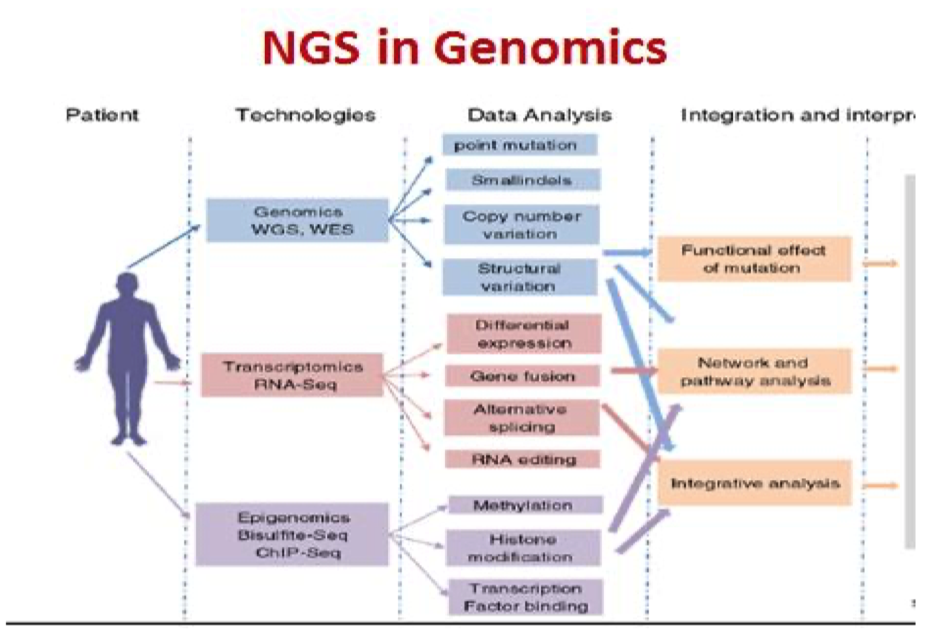
\includegraphics[width=\textwidth]{NGS_data}
  \caption[NGS data analysis classification]{
    NGS data analysis classification. The figure is from \url{http://www.biostat.jhsph.edu/~khansen/enar2012.html}.
  }
  \label{fig:NGS_data}
\end{figure}

Apart from multiple genomics data types generated from modern technologies, these data has their own underlying characteristics. Genomic annotation databases contains information about biological pathways and functional gene sets indicating a group of genes working collectively on one particular functionality. Examples of such annotation data bases are molecular signature database (MSigDB), gene ontology databases such as KEGG and reactome, and the chromosome on which a gene is located. There are also summary statistics like p-values, odds ratios, hazard ratios from external studies with related objective on the same set of genomics data. These information highlights the characteristics of genomic features, which are the features of genomic features. We call them meta-features from here and after. The meta-features reveal information on two fundamental characteristics of genomics, grouping and ordering. Gene annotations provide grouping information related to disease traits, while summary statistics provide ordering of genomic features, which indicates the importance of the features for a class of disease. 

Among the more important uses of these discoveries is providing detailed, mechanistic insight into the molecular pathogenesis of disease states. The two primary avenues of utilizing this explosion in genomics information for the purpose of improving clinical practices are in (1) prediction of disease prognostics, pharmacogenetic response, and disease severity/trajectory (2) prediction of treatment effects on individuals with certain genomic profiles and clinical features. Much of the variation in disease course, severity, and response to medication is reflective of the underlying genomic profile existing in each individual, offering the opportunity for genomics to facilitate early treatment, preventative medicine, preemptive selection of efficacious drugs, and more accurate estimation of risk for those thought to be at intermediate risk using traditional factors.

With the huge amount of genomics data in multiple categories, and ever growing annotation databases, the purpose of this thesis is to integrate multiple types of genomics data, meta-features into predictive modeling process, in the hope of improving model prediction performance, producing interpretable results (feature-selection).

\section{Genomics-based prediction of disease traits}
\label{sec:Prediction}
In the contest of discovering disease prognostic factors, predictive signals, predictive models are methods designed to use clinical, genomics, or other types of data for the purpose of forecasting a medical trait. Predictive models are most beneficial when they yield actionable and personalized results. They are of reduced value  if they only substantially modify medical decisions for a small fraction of the patient population. Therefore, the ideal genomics-based predictive model for clinical applications (1) substantially modifies the probability of medical traits upon which medical decisions based compared to that obtained from existing clinical assessment and tests, and (2) impacts a large fraction of individuals to whom it is applied and provides improved outcomes. Given that for many disease with multiple treatment strategies, accurate prediction of disease traits can play a critical role in determining robust clinical care that may avert severe disease, prolong survival, or even prevent disease onset. 

In this thesis, the focus is on cancer genomics applications. As the advent of genetic testing in tumor cells, through harnessing the throughput and read depth of NGS platforms, it has enabled detailed and clinically actionable molecular pathology genetic tests for numerous cancers. Multiplex sequencing-based assays for biopsies compared to normal tissue are now available and have demonstrated usefulness in augmenting many clinical decisions.

We give a brief overview of some of the high profile predictive modeling techniques for genomics. 

\subsection{Genome-wide association studies}
In an attempt to develop such predictive models, many have used genome-wide association study (GWAS). It is an approach used in genetics research to associate specific genetic variations with particular diseases \citep{manolio2010genomewide}. The method involves scanning the genomes from many different people and looking for genetic markers that can be used to predict the presence of a disease. Those genetic markers, either used alone or combined with traditional non-genetic risk prediction, have the potential to improve risk-prediction accuracy, which might benefit clinical diagnose and personalized treatment.

To carry out a genome-wide association study, two groups of subjects are identified: people with the disease being studied (cases) and similar people without the disease (controls); or people with different phenotypes for a particular trait, for example blood pressure, are identified. Each subject's complete set of DNA, genome is acquired and microarray chip technology or WGS, WES are applied to obtain common genetic variations, SNPs. It scans the entire genome to find statistically significant variations that are associated with the disease, using some form of family-wise error rate control.  

The discovery of genetic markers for the prediction of disease traits is entirely dependent on the underlying genetic model that gives rise to the trait. That is, the number of loci and the frequency and penetrance of predisposing alleles determine both the likelihood of identifying causal markers and the clinical utility of using those markers in a patient population. For example, monogenic disorders are very likely fully penetrant with allele frequencies that are not exceedingly rare, therefore, genetic tests for such diseases have clinical applications provided that disease prevention or disease trait dependent treatment exists. On the other hand, there are complex diseases that follow, e.g., weakly penetrant alleles, several hundreds to thousands loci, ubiquitous epigenetic effects, gene-environment interactions, or some combination hence, directly impacts the identification of predictive markers. GWAS interrogate the common allelic architecture for disease traits, whereas sequencing-based studies in families can facilitate the discovery of rare disease-associated variants, but are not optimal for identifying ancestral disease-predisposing alleles. Therefore, it is reasonable to expect that genetic markers from GWAS may apply to a large segment of individuals, but with a mild impact on the probability of disease traits.

\subsection{Regression}
Regression methods, linear models, are common techniques for constructing predictive models. For quantitative traits, it is linear regression; for dichotomous traits, logistic regression is deployed; for survival traits, Cox's proportional hazards regression, parametric regression models with various survival time distribution assumptions are for choices. Regression methods construct likelihood functions based on linear predictors. The input is a response vector $\bm{Y}$ of length $n$ (for survival outcomes, it is a response matrix of dimension $n \times 2$, survival time and censoring status) and a data/design matrix $\bm{X}$ of dimension $n \times p$, where $n$ is the number of independent samples, $p$ is the number of features. Then the linear predictors for each of the $n$ samples are defined as $\bm{\beta}^T\bm{x}_i$, where $\bm{x}_i$ is the features for the $i$th sample, $\bm{\beta}$ is the regression coefficients to be estimated. Negative log likelihood for each of the outcome types are listed below, i.e, the optimization problems for each of the regression models:
\begin{align}
    &\min_{\bm{\beta}} \left\{\frac{1}{2n} \sum_{i=1}^{n} (y_i-\bm{\beta}^T\bm{x}_i)^2 \right\}, \qquad\qquad\qquad\quad\;\: \text{linear regression} \label{eq1.1} \\
    &\min_{\bm{\beta}} \left\{-\frac{1}{n} \sum_{i=1}^{n} \left[y_i\bm{\beta}^T\bm{x}_i-\ln(1+e^{\bm{\beta}^T\bm{x}_i})\right]\right\}, \qquad \text{logistic regression} \label{eq1.2}
\end{align}
Cox's proportional hazards regression will be showed in detail in the following sections as the main medical traits to be dealt with. Incorporation of covariates and interaction effects are possible with regression, as opposed to GWAS, risk predictions are given by effect sizes of each significant hits.

There are several assumptions made when applying regression. First, the number of features $p$ should be less than the number of samples $n$ for the model to be able to fit. However, this is usually not the case in genomics study. DNA information are typically acquired by tissue biopsy in cancer patients. The biopsies could be highly invasive depending on the location of tumors, hence not feasible for everyone. Also, there are concerns for DNA sequencing cost. As a result, the number of samples is small to moderate at best, typical number ranges from hundreds to thousands. On the contrary, the number of genomic features is huge. There may be tens and hundreds of thousands genetic variations. If there are multiple types genomics including gene expressions, methylations and so on, the number is even larger. Therefore, genomics data are high dimensional ($p>>n$) in most cases. Multicollinearity between nearby markers is another serious concern. Highly correlated markers should have similar regression coefficients (negatively correlated markers have opposite sign, but similar in magnitude), i.e., a group of correlated markers share the group effect size equally. But in regression, the coefficient estimates are highly unstable given high correlation. Other concerns include marker-marker interactions, missing data. 

\subsection{Other machine learning methods}
Diagnosis and prognostic of disease traits with genomics information are classification and clustering problems within machine learning. Therefore, methods such as tree-based including random forest, gradient boosting machines, support vector machines, neural networks can be applied to these tasks. One of the applications in this category is Bayesian networks resulted from graph theory and applied probability \citep{jordan2004graphical}. Take a simplified version as an example, if the genomic features can be reasonably assumed independent conditional on disease traits, the network reduced to a naive Bayes model. Given a set of $p$ genomic features, the posterior probability of disease trait is:
\begin{align*}
    P(D|\cap_{i=1}^n G_i)&=\frac{P(\cap_{i=1}^n G_i|D)P(D)}{P(\cap_{i=1}^n G_i)} \\
    &=\frac{P(D=1)\prod_{i=1}^n P(G_i|D=1)}{P(D=1)\prod_{i=1}^n P(G_i|D=1)P(D=0)\prod_{i=1}^n P(G_i|D=0)}
\end{align*}
This carries some interpretability since the posterior probability tells some stories of how the genomic features contribute to disease traits. However, it is not as flexible in learning underlying non-linear patterns as its counterparts, tree-based, neural networks. It learns quadratic pattern and linear pattern when assuming equal variance of $G_i|D$, which shares some similarity with quadratic/linear discriminant analysis.

\subsection{Comparison of predictive methods in genomics}
Considering the high-dimensionality of genomics data, every genomic feature contribute a little to none effect to disease traits. Hence, there is not much effect either to contribute to square, square root of genomic features, etc., the non-linear patterns of features. Gradient boosting machine, neural network are superior when sample size is large, since there is enough information for them to explore complicated non-linear patterns. On the other hand, regression represents the genomic feature effects very well. Regression coefficients are effects to disease traits, they can be small to zero. This is the reason why regression is still the most widely used model in genomics, instead of tree-based methods and neural networks, despite their huge success in other areas.

GWAS scanned the whole genome one at a time to find significant hits after controlling for family-wise error rate, typically controlling for false discovery rate to allow more power to detect associated SNPs. With GWAS, only effect sizes of single signals are given, while regression has the ability to build a multivariate model for all detected signals and other covariates to be controlled, and also makes it possible to explore gene-gene, gene-environment interactions. However, in most cases, the combined effects of genetic markers found by GWAS explain a small proportion of inter individual differences in genetic risk. In part, this reflects lack of power of standard GWAS to detect small effect markers. A number of studies have shown that prediction accuracy can be increased by including in the model markers that may not show significant association at the marginal level, e.g., \citep{allen2010hundreds}. This brings out the key question in building predictive models in genomics, feature selection: which genomic features are most effective in determining the disease traits and should therefore be included in a predictive model.

The goal is to build a predictive model including genomic features collectively contribute most to disease trait, so as to maximize model's predictive power. One strategy is to include all genomics information at hand, and let the model decide which features are in the model to achieve optimal prediction performance. We know regression cannot be fit with high-dimensional data. Therefore, regularization need to be introduced. 

\section{Regularized regression}
Considering a linear regression, equation \eqref{eq1.1}, the solution to it is the ordinary least square (OLS), $\hat{\bm{\beta}}=(\bm{X}^T\bm{X})^{-1}\bm{X}^T\bm{Y}$. If $\bm{X}_{n\times p}$ is high-dimensional, $p>n$, the highest rank of matrix $(\bm{X}^T\bm{X})_{p\times p}$ is $\min(p,n)=n$, so it is a singular matrix. Mathematically, there is no solution to $\bm{\beta}$. Intuitively, the model is too complex to fit because there is not enough data. Regularization is a technique to control model complexity, by shrinking the regression coefficients. Regularized regression can be written as:
\begin{equation}
    \min_{\bm{\beta}} \left\{\ell(\bm{\beta)} + \lambda P(\bm{\beta)}\right\}, \label{eq1.3}
\end{equation}
where $\ell(\bm{\beta)}$ is the loss function/negative log likelihood. $P(\bm{\beta)}$ is the regularization/penalty function, which penalizes regression coefficients so that the estimates of coefficients shrink, making the model simpler.  $\lambda \geq0$ is a hyperparameter that controls amount of shrinkage, thus controls the model complexity. There are many type of penalty functions, we will look at some of the high profile types of regularization.

\subsection{Ridge regression}
Ridge regression is proposed by \cite{hoerl1970ridge}. It shrinks the regression coefficients by imposing a regularization/penalty on their size. The ridge coefficients minimize a regularized loss function,
\begin{equation}
    \min_{\bm{\beta}} \left\{ \ell(\bm{\beta})+\lambda\|\bm{\beta}\|_2^2  \right\}. \label{eq1.4}
\end{equation}
The larger the value of $\lambda$, the greater the amount of shrinkage on coefficients $\bm{\beta}$. The coefficients are shrunk toward zero. An equivalent way to write the ridge problem is 
\begin{equation}
    \begin{aligned}
    &\min_{\bm{\beta}} \ell(\bm{\beta}), \\
    &\text{subject to} \qquad \|\bm{\beta}\|_2^2 \leq t, \label{eq1.5}
    \end{aligned}
\end{equation}
which makes explicit the size constraint on the coefficients. There is a one-to-one correspondence between the parameters $\lambda$ and $t$. Where there are many correlated features in a standard regression model, their coefficients can be unstable due to high variance. By imposing a size constraint, the problem is alleviated. 

The solution to the ridge optimization problem is $\hat{\bm{\beta}}^{ridge}=(\bm{X}^T\bm{X}+\lambda \bm{I})^{-1}\bm{X}^T\bm{Y}$. Like the OLS solution, ridge regression solution is also a linear function of outcome $\bm{Y}$. It adds a positive constant $\lambda$ to the diagonal of $\bm{X}^T\bm{X}$ before inversion, making the matrix nonsingular even if $\bm{X}^T\bm{X}$ is not of full rank (high-dimensional setting). This is how ridge regression fit high-dimensional data and other ill-formed design matrix $\bm{X}$. In the case of orthonormal column spaces of $\bm{X}$, the ridge solution becomes a scaled version of the OLS solution, i.e., $\hat{\bm{\beta}}^{ridge}=\frac{1}{1+\lambda}\hat{\bm{\beta}}^{OLS}$, shrinking the coefficients by a fraction of $1+\lambda$. If the column spaces of $\bm{X}$ are not othonormal, ridge regression shrinks the directions with smallest variances the most. Those directions are in fact the principle components directions of $\bm{X}$. The first principle component has the largest sample variance (eigen value) amongst all normalized linear combinations of the columns of $\bm{X}$. Subsequent principal components have maximum variance subject to being orthogonal to the earlier ones. Hence, the small eigen value principle components directions are shrunk the most. 

Ridge regression has a Bayesian interpretation, assuming linear regression:
\begin{align*}
    &\bm{Y}|\bm{\beta};\bm{X} \sim N(\bm{X\beta}, \sigma^2\bm{I}), \\
    &\pi(\bm{\beta}) \sim N(0, \gamma^2\bm{I}).
\end{align*}
Both likelihood and prior are normal, therefore, the posterior distribution is also a normal. Because normal is its own conjugate family. The negative log posterior density of $\bm{\beta}$ is equal to the expression in equation \eqref{eq1.4}, with $\lambda=\sigma^2/\gamma^2$. Thus the ridge estimate is the mean and mode of the posterior distribution. In genomics, Bayesian ridge regression is the motivation of genomic best linear unbiased predictor (G-BLUP) \citep{de2013prediction}. 

Ridge regression shrinks coefficients toward zero, but never to exactly zero. In other words, it doesn't perform feature selection in terms of magnitude of regression coefficients. If coefficients shrink to zero, these features are no longer in the model, and thus not associated with outcome. Features with larger coefficients in magnitude, weather positive or negative, are strongly associated with outcome. However, ridge regularization is a widely used technique for controlling model complexity to balance the trade-off between bias and variance. The more complex the model, the less bias, but the larger variance, and vice versa. It is used in neural networks and gradient boosting machines, where it is known as weight decay.    

\subsection{Sparse regularized regression and feature selection}
\subsubsection{The Lasso}
Proposed by \citep{tibshirani1996regression}, the lasso is a regularization method like ridge, but performs feature selection. The lasso optimization problem, Lagrangian form, is defined as 
\begin{equation}
    \min_{\bm{\beta}} \left\{ \ell(\bm{\beta})+\lambda\|\bm{\beta}\|_1  \right\}. \label{eq1.6}
\end{equation}
It can also be written in the equivalent constrained optimization problem just like ridge,
\begin{equation}
    \begin{aligned}
    &\min_{\bm{\beta}} \ell(\bm{\beta}), \\
    &\text{subject to} \qquad \|\bm{\beta}\|_1 \leq t. \label{eq1.7}
    \end{aligned}
\end{equation}
The similarity to the ridge regression is the $L_2$ norm penalty function for ridge is replaced by $L_1$ norm penalty function for the lasso. The term sparse refers to a model with few nonzero coefficients. A key property of the lasso is its ability to yield sparse solutions. Lets look at the lasso estimator for linear regression. For the $j^{th}$ feature, i.e, the $j^{th}$ element of coefficients vector $\bm{\beta}$, the coordinate-wise update, for standardized features with mean 0 and variance 1, has the form
\begin{equation}
    \hat{\beta}_j^{lasso}=S(\frac{1}{n}\sum_{i=1}^{n}x_{ij}r_i^{(j)}, \lambda) \label{eq1.8}
\end{equation}
where 
\begin{itemize}
    \item $r_i^{(j)} = y_i-\sum_{l\neq j}x_{il}\hat{\beta}_l$ is the partial residual which removes from the outcome the current fit from all but the $j^{th}$ predictor. Because features are usually standardized to make the shrinkage comparable, $\frac{1}{n}\sum_{i=1}^{n}x_{ij}r_i^{(j)}$ is the simple least squares solution when fitting this partial residual to $x_{ij}$.
    \item $S(x, \lambda)$ is the soft-thresholding operator defined as 
    \begin{equation}
        \text{sign}(x)(|x|-\lambda)_+ = 
            \begin{cases}
                x-\lambda & \text{if $x>0$ and $\lambda<|x|$}\\
                x+\lambda & \text{if $x<0$ and $\lambda<|x|$}\\
                0 & \text{if $\lambda \geq |x|$}
            \end{cases} \label{eq1.9}      
    \end{equation}
\end{itemize}
One can derive the results using the notion of subgradients, the detailed derivation of coordinate descent are described in \cite{friedman2007pathwise}. Notice the lasso solution shrinks the regression coefficient (solution of least squares, $\frac{1}{n}\sum_{i=1}^{n}x_{ij}r_i^{(j)}$) by an amount of $\lambda$, as long as its magnitude/absolute value is larger than $\lambda$. For the features having smaller effect sizes than $\lambda$, they are shrunk to 0, thus being excluded to the model (Figure \ref{fig:soft_threshold}). This is the main difference between ridge and the lasso, while ridge regression does a proportional shrinkage, lasso translates each coefficient by a constant $\lambda$, truncating at zero. Therefore, the lasso has the ability to perform feature selection by excluding unimportant features. In this way, the lasso model is more parsimonious, more interpretable, compared to ridge, which keeps all the features in the model.
\begin{figure}[tbh]
  \centering
  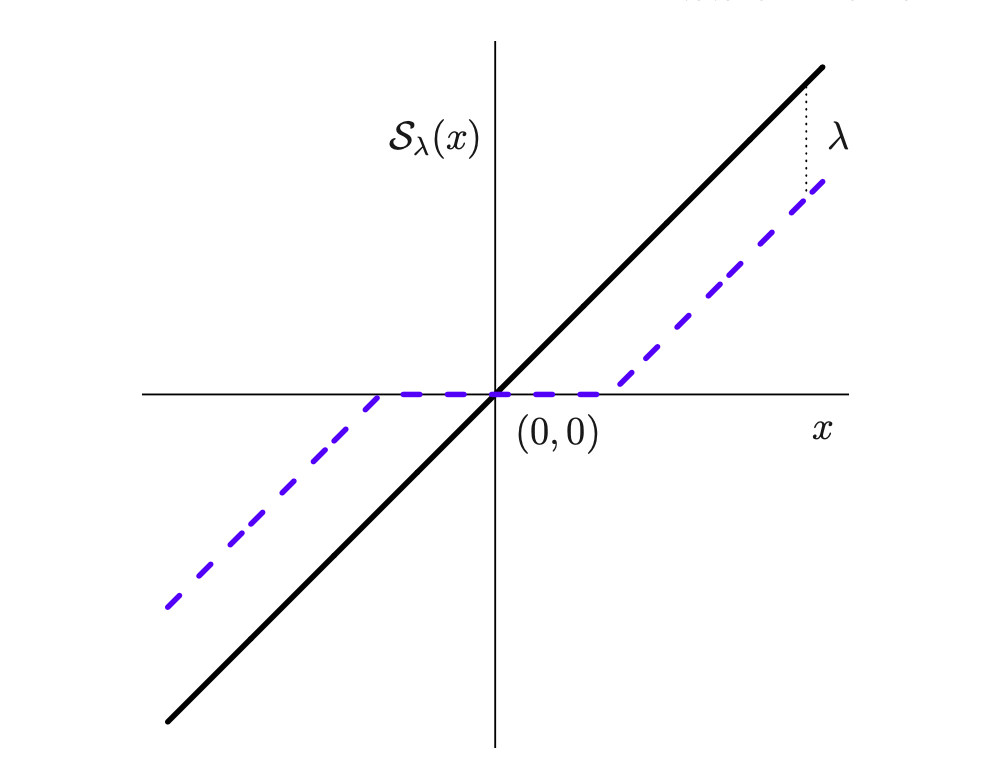
\includegraphics[scale=0.6]{soft_threshold}
  \caption[Soft thresholding function $S(x, \lambda)=\text{sign}(x)(|x|-\lambda)_+$]{
    Soft thresholding function $S(x, \lambda)=\text{sign}(x)(|x|-\lambda)_+$. The figure is from \cite{hastie2019statistical}. The blue broken line is the soft threshoding estimator, along with the $45^{\circ}$ line in black.
  }
  \label{fig:soft_threshold}
\end{figure}

There are some important properties of the lasso in addition to feature selection.
\begin{itemize}
    \item Just like ridge regression, the lasso also has an Bayesian interpretation. The prior distribution of $\bm{\beta}$ is double exponential/Laplace for the lasso, instead of normal for ridge.
    \item Degrees of freedom: Suppose there are $p$ features, fitting a linear regression using only a subset of $k$ of these features, if these $k$ features were chosen without regard to the outcome, the procedure spends $k$ degrees of freedom. However, if the $k$ features were chose using knowledge of the outcome, for example best subset selection, then the fitting procedure spends more than $k$ degrees of freedom. Such a fitting strategy is adaptive, as well as the lasso. The lasso, with a fixed penalty parameter $\lambda$, the number of nonzero coefficients $k_\lambda$ is an unbiased estimate of the degrees of freedom \citep{zou2007degrees, tibshirani2012degrees}. The reason that lasso has exactly $k$ degrees of freedom rather than larger than $k$ is that it not only selects features which inflates the degrees of freedom, but also shrinks the coefficients. This result gives us a qualitative measure of the amount of fitting having been done at any point along the lasso path.
    \item The number of nonzero coefficients is at most $n$, the sample size, when the data is high dimensional, $p>n$.
    \item Assume that the underlying true signal is sparse, the lasso recovers the true signals well. If the underlying truth is not sparse, the lasso does not work well. 
\end{itemize}

\subsubsection{The elastic net}
Proposed by \cite{zou2005regularization}, the elastic net makes a compromise between the ridge and the lasso; it solves the convex optimization problem
\begin{equation}
    \min_{\beta} \left\{ \ell(\bm{\beta})+\lambda\left[\frac{1}{2}(1-c)\|\bm{\beta}\|_2^2+c\|\bm{\beta}\|_1\right] \label{eq1.10} \right\} 
\end{equation}
where $c\in [0,1]$ is a parameter that controls whether the penalty function to be more close to lasso or more close to ridge. When $c=1$, it reduces to $L_1$ norm, lasso penalty; when $c=0$, it reduces to squared $L_2$ norm, ridge penalty. The coordinate-wise update for the elastic net linear regression, again assuming the features are standardized to mean 0 and variance 1, is 
\begin{equation}
    \hat{\beta}_j^{enet} = \frac{S(\frac{1}{n}\sum_{i=1}^{n}x_{ij}r_i^{(j)}, \lambda c)}{1+\lambda(1-c)} \label{eq1.11}
\end{equation}
We can see the elastic net estimator shrinks the regression coefficients in the way of both lasso and ridge: it has the soft-thresholding portion truncating at $\lambda c$; it also shrink the coefficients proportionally with a factor of $1+\lambda(1-c)$. Hence, the elastic net shrinks the coefficients and some of them to exactly 0, so feature selection.

\subsection{Discussion of ridge regression, the lasso, the elastic net, and best subset selection}
Best subset selection finds for each $k\in\{0,1,2,\dots,p\}$ the subset of size $k$ that gives smallest residual sum of squares (validation error). Best subset selection linear regression is equivalent to $L_0$ constrained regression, when design matrix $\bm{X}$ is orthogonal:
\begin{equation}
\begin{aligned}
    &\min_{\bm{\beta}} \frac{1}{2n}\|\bm{Y}-\bm{X\beta}\|_2^2, \\
    &\text{subject to} \quad \|\bm{\beta}\|_0 \leq k, \label{eq1.12}
\end{aligned}
\end{equation}
where $\|\bm{\beta}\|_0=\sum_{j=1}^p I(\beta_j \neq 0)$, is defined as the number of nonzero coefficients. Strictly speaking, $L_0$ is not a norm because it does not have properties of a norm, but the naming and notation are widely used. The $L_0$ constraint penalizes the number of nonzero coefficients, instead of the magnitude of coefficients. This exactly describes the best subset selection setting. And because it does not shrink the coefficients, the $L_0$ estimates are unbiased, while other regularization estimates are biased toward 0. Although, best subset selection, or $L_0$ constrained regression is superior in coefficient estimation, feature selection, it does not have an efficient algorithm, when $\bm{X}$ is not orthogonal. If we want to select a best subset without knowing how many features should be included to be the best subset, $k$, then there are $2^p$ combinations of features need to be examined. In other words, there are no polynomial time algorithm to solve it; the problem is NP-hard. Many approximation methods have been proposed to solve the problem. Among them, iterative hard thresholding is well performed. The closed form hard thresholding solution for $L_0$ constrained linear regression when $\bm{X}$ is orthogonal is   
\begin{equation}
    \hat{\bm{\beta}}^{L_0}=H_{\sqrt{2\lambda}}(\frac{1}{n}\bm{X}^T\bm{Y}), \label{eq1.13}
\end{equation}
where $H_{\sqrt{2\lambda}}(\cdot)$ is the hard thresholding operator,
\begin{equation}
    H_{\sqrt{2\lambda}}(\frac{1}{n}\bm{X}^T\bm{Y})=
    \begin{cases}
        \frac{1}{n}\bm{X}^T\bm{Y} & \text{if $|\frac{1}{n}\bm{X}^T\bm{Y}|>\sqrt{2\lambda}$}, \\
        0 & \text{if $|\frac{1}{n}\bm{X}^T\bm{Y}|\leq\sqrt{2\lambda}$}.
    \end{cases}
\end{equation}
It does not shrink regression coefficients at all, but truncates at $\sqrt{2\lambda}$. This is in close relation to the soft thresholding estimator of lasso, equation \eqref{eq1.9}, which shrinks coefficients by the amount of $\lambda$ and truncates at $\lambda$. This is why hard thresholding is an unbiased estimator of regression coefficient. In fact, the lasso is one of many approximations to $L_0$ constrained problem. And it is the closest convex approximation to it, while $L_0$ is a nonconvex optimization problem. Figure \ref{fig:estimators} shows the estimators for best subset/$L_0$, ridge, and lasso in the case of orthonormal orthogonal $\bm{X}$. We can see the unbiased estimator of best subset; feature selection ability of best subset and lasso; and different shrinkage scheme between ridge and lasso.
\begin{figure}[tbh]
  \centering
  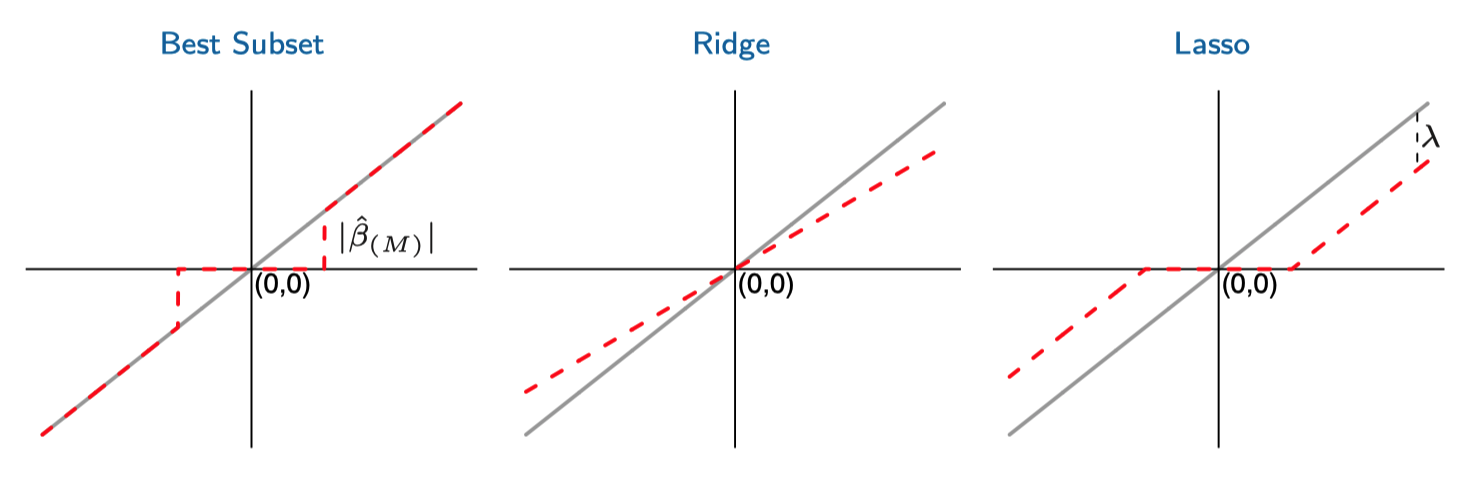
\includegraphics[scale=0.6]{estimator}
  \caption[Estimators of $\beta_j$ in the case of orthonormal columns of $\bm{X}$]{
    Estimators of $\beta_j$ for best subset, ridge, lasso, in the case of orthonormal columns of $\bm{X}$. Estimators are shown by broken red lines. The figure is from \cite{hastie2009elements}.
  }
  \label{fig:estimators}
\end{figure}

Ridge regression and the elastic net are also convex optimization problems. Since ridge, lasso and elastic net share this nice property, they have a highly efficient computational algorithm in pathwise coordinate descent \citep{friedman2007pathwise}. The algorithm solves the problems along a decreasing sequence of $\lambda$ values, for the purpose of tuning $\lambda$ via cross validation. Apart from giving a path of solutions, the algorithm exploits warm start, which initializes $\hat{\bm{\beta}}$ with the solutions of previous $\lambda$ value. This works because convex objective functions have continuous solutions along the path. By starting at previous solutions, coordinate descent updates need less iterations, thus leads to a more efficient and stable algorithm. On the other hand, iterative hard thresholding is not as efficient, and only guarantees to reach local minimums due to $L_0$'s nonconvexity. 

The lasso does not deal with highly correlated features very well; the solutions tend to be unstable. If there is a group of variables among which the pairwise correlations are very high, then the lasso tends to select only one variable from the group and does not care which one is selected. Ridge regression is known to shrink the coefficients of correlated features towards each other, allowing them to borrow strength from each other. In the extreme case of $k$ identical features, they each get identical coefficients with $1/k$ the size that any single one would get if fit alone. The elastic net is a combination of ridge and lasso. It selects features like the lasso, and shrinks together the coefficients of correlated features like ridge. As $c$ increases from 0 to 1, for a given $\lambda$, the sparsity of the elastic net solution, i.e., the number of coefficients equal to zero, increases monotonically from 0 to the sparsity of the lasso solution. 

\subsection{Nonconvex regularized regression}
Ridge regression, the lasso, the elastic net are all convex optimization problems. There are stable and efficient algorithms to solve it. And they always reach their global minimum solutions. Because of these, they are widely used for regularization, controlling model complexity. However, by moving from $L_2$ ridge to $L_1$ lasso, we have seen the lasso selects a subset of features to have nonzero coefficients, and shrinks them. When the number of features is large and the number of relevant features is small, this may not be enough. In order to reduce the set of chosen features sufficiently, lasso may end up over-shrinking the retained features. Nonconvex regularization leads to more sparse, less biased solutions. To see this, consider $L_q$ regularization,
\begin{equation}
    \min_{\bm{\beta}} \left\{ \frac{1}{2n}\|\bm{Y} - \bm{X\beta}\|_2^2 + \lambda \sum_{j=1}^{p}|\beta_j|^q \right\} \label{eq1.15}
\end{equation}
for $q\geq0$. It is the lasso for $q=1$, ridge for $q=2$. Figure \ref{fig:lq} displays $L_q$ regularization in the case of two inputs. For $0 \leq q <1$, the regularization is nonconvex, with the limiting $q=0$ corresponding to best subset selection. For these nonconvex constraints, they concentrate more mass in the coordinate directions, thus the solutions tend to be more sparse, and less shrinkage (biased toward 0). Unfortunately, along with nonconvexity comes combinatorial computational complexity and unstable algorithms. Alternatives nonconvex regularization have been proposed.
\begin{figure}[tbh]
  \centering
  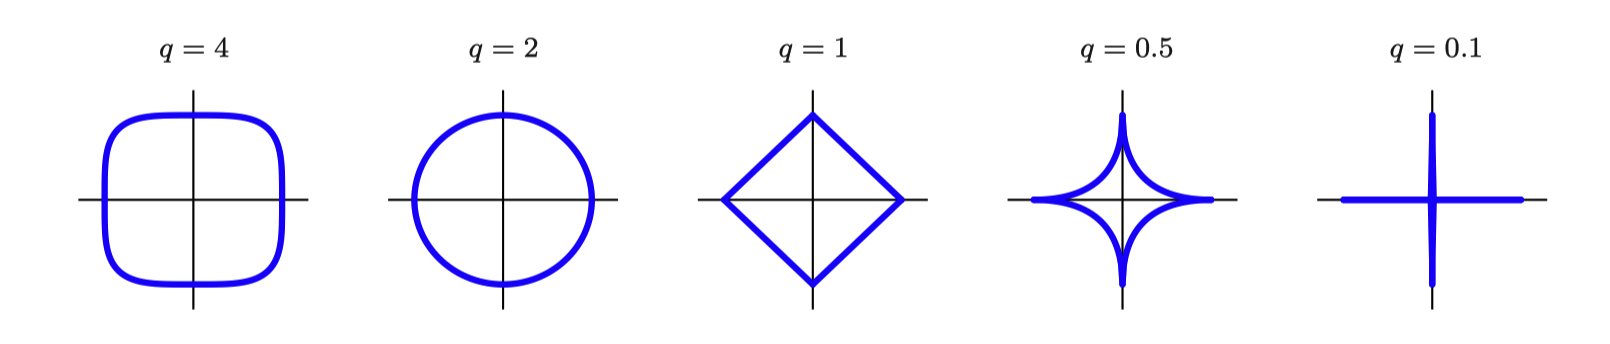
\includegraphics[width=\textwidth]{lq}
  \caption[Constraint regions $\sum_{j=1}^p|\beta_j|^q\leq1$ for different values of $q$] {
    Constraint regions $\sum_{j=1}^p|\beta_j|^q\leq1$ for different values of $q$. For $q<1$, the constraint region is nonconvex. The figure is from \cite{hastie2009elements}. 
  }
  \label{fig:lq}
\end{figure}

\subsubsection{Smoothed clipped absolute deviation penalty (SCAD) and minimax concave penalty (MCP)}
Proposed by \cite{fan2001variable}, the SCAD penalty defined on $[0, \infty)$ is given by (symmetric on $(-\infty, 0)$)
\begin{equation}
    P_{\lambda,\gamma}(\beta) = 
        \begin{cases}
            \lambda\beta & \text{if $\beta \leq \lambda$}\\
            \frac{\gamma\lambda\beta-0.5(\beta_2+\lambda^2)}{\gamma-1} & \text{if $\lambda<\beta\leq\gamma\lambda$}\\
            \frac{\lambda^2(\gamma^2-1)}{2(\gamma-1)} & \text{if $\beta>\gamma\lambda$}
        \end{cases} \label{eq1.16}      
\end{equation}
for $\lambda\geq0$ and $\gamma>2$. The univariate solution for a SCAD regularized simple linear regression coefficient is as follow
\begin{equation}
    \hat{\beta}=f_{SCAD}(z,\lambda,\gamma)= 
        \begin{cases}
            S(z,\lambda) & \text{if $|z|\leq 2\lambda$}\\
            \frac{S(z, \gamma\lambda/(\gamma-1))}{1-1/(\gamma-1)} & \text{if $2\lambda<|z|\leq\gamma\lambda$}\\
            z & \text{if $|z|>\gamma\lambda$}
        \end{cases} \label{eq1.17}      
\end{equation}
where $z=\frac{1}{n}\bm{X}^T\bm{Y}$ is the OLS solution.

Proposed by \cite{zhang2010nearly}, the MC+ penalty defined on $[0, \infty)$ is given by (symmetric on $(-\infty, 0)$)
\begin{equation}
    P_{\lambda,\gamma}(\beta) = 
        \begin{cases}
            \lambda\beta - \frac{\beta^2}{2\gamma} & \text{if $\beta \leq \gamma\lambda$}\\
            \frac{1}{2}\gamma\lambda^2 & \text{if $\beta>\gamma\lambda$}
        \end{cases} \label{eq1.18}      
\end{equation}
for $\lambda\geq0$ and $\gamma>1$. The univariate solution for a MC+ regularized simple linear regression coefficient is as follow
\begin{equation}
    \hat{\beta}=f_{MCP}(z,\lambda,\gamma)= 
        \begin{cases}
            \frac{S(z,\lambda)}{1-1/\gamma} & \text{if $|z|\leq \gamma\lambda$}\\
            z & \text{if $|z|>\gamma\lambda$}.
        \end{cases} \label{eq1.19}      
\end{equation}

The rational of SCAD and MCP is similar in that both penalties begin by applying same penalty as the lasso, and reduce the amount of penalty as the regression coefficient gets further away from zero. As a result of the penalty trend, when the coefficient is small in magnitude, it is shrunk to zero just like lasso; however, when the coefficient is large (larger than OLS solution), there is a transition region that shrinks the coefficient less than the lasso, and after the transition region, it is equal to the OLS solution without any shrinkage. This is a trend from less biased toward 0 to unbiased estimator, for those features with large effect sizes, thereby more likely to be associated with outcomes. Without the transition region, it is the hard thresholding estimator. The difference between SCAD and MCP is in the way they make transition. Figure \ref{fig:nonconvex_est} shows the trend of penalty functions of SCAD, MCP and their threshold functions. Indexed by nonconvexity parameter $\gamma$, it bridges the gap between lasso ($\gamma=\infty$) and best subset/hard threshold ($\gamma=2_+$ for SCAD $1_+$ for MCP).   
\begin{figure}[tbh]
  \centering
  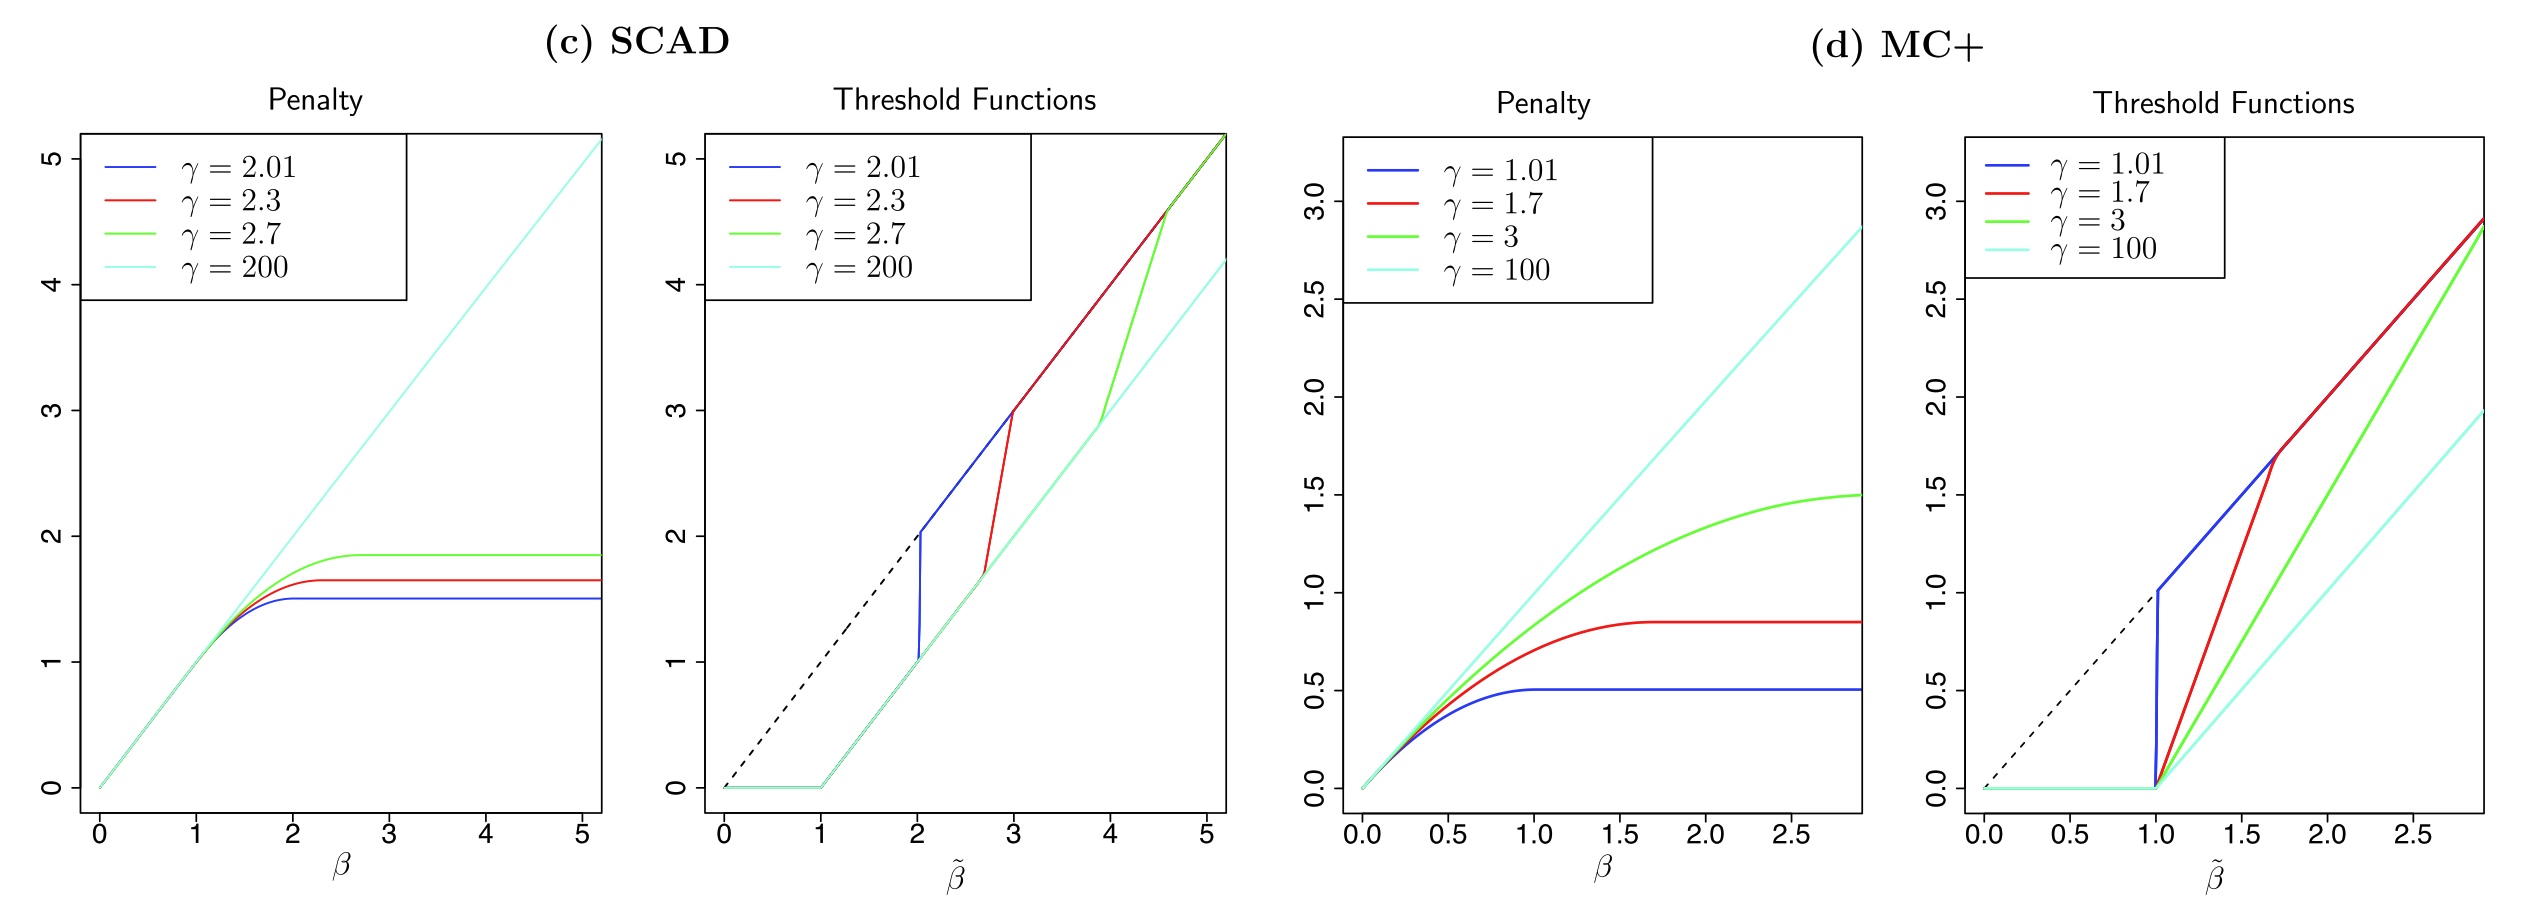
\includegraphics[width=\textwidth]{nonconvex_est}
  \caption[SCAD and MCP penalty functions and their corresponding threshold functions] {
    SCAD and MCP penalty functions and their corresponding threshold functions. Both are shown with $\lambda=1$ and different values for $\gamma$. The figure is from \cite{mazumder2011sparsenet}. 
  }
  \label{fig:nonconvex_est}
\end{figure}

The two nonconvex regularization techniques achieve less biased estimator, more sparse subset than the lasso. The choice of convex and nonconvex regularization depends on the application. For example, for a gene expression profile data, the underlying model is sparse but with a relatively large subset of features, the lasso is a better choice. Because with a large number of features in the model, say $1000-2000$, the direction of the feature coefficients are more meaningful rather than the magnitude of the coefficients. For a genetic association data, by which the underlying model only consists of a few markers, the accuracy of selection and unbiasedness of estimators are important. Hence, nonconvex regularization is a better suit in the situation.

We close the section by mentioning an approximation to $L_q$ ($0\leq q <1$) regularization that enjoys convex property.

\subsubsection{The adaptive lasso: approximation to nonconvex regularization}
Proposed by \cite{zou2006adaptive}, the adaptive lasso is a way of fitting models sparser than lasso. Using a pilot estimate $\tilde{\beta}$, the adaptive lasso has the form
\begin{equation}
    \min_{\bm{\beta}} \left\{ \frac{1}{2n}\|\bm{Y}-\bm{X\beta}\|_2^2+\lambda\sum_{j=1}^pw_j|\beta_j| \right\}, \label{eq1.20}
\end{equation}
where $w_j=1/|\tilde{\beta}_j|^v$. The adaptive lasso can be seen as an approximation to the $L_q$ regularization with $q=1-v$. We can see the adaptive lasso is convex in $\bm{\beta}$. Moreover, when the pilot estimates meet some regulatory conditions, the method recovers the true model under more general conditions than does the lasso. One can use least squares solution as the pilot estimate when $p<n$, univariate least squares solution when $p\geq n$. The indication is that, when least squares solution is small, the amount of penalty $w_j$ for feature $j$ is large, thereby $\hat{\beta}_j$ is more likely to be set to 0; when least squares solution is large, feature $j$ is penalized less (small $w_j$), then $\hat{\beta}_j$ is shrunk less, making it less likely to be 0 and less biased.

% Research Topic 1
\chapter{A Regularized Cox’s Hierarchical Model for Incorporating Annotation Information in Omics Studies}
\label{cha:xrnetcox}

\section{Abstract}
Associated with high-dimensional omics data there are often “meta-features” such as pathways and functional annotations that can be informative for predicting an outcome of interest. We extend to Cox regression the regularized hierarchical framework of Lee et al. [ ] for integrating meta-features, with the goal of improving prediction and feature selection performance with time-to-event outcomes. Regularization is applied to the omic features as well as the meta-features so that high-dimensional data can be handled at both levels. The proposed hierarchical Cox model can be efficiently fitted by a combination of iterative reweighted least squares and cyclic coordinate descent. In a simulation study we show that when the external meta-features are informative, the regularized hierarchical model can substantially improve prediction performance over standard regularized Cox regression. Importantly, when the external meta-features are uninformative, the prediction performance based on the regularized hierarchical model is on par with standard regularized Cox regression, indicating robustness of the framework. We illustrate the proposed model with applications to prediction of breast cancer survival, prediction of overall survival of melanoma, based on gene expression.

\section{Introduction}
Prediction based on high-dimensional omics data such as gene expression, methylation, and genotypes are important for developing better prognostic and diagnostic signatures of health outcomes. However, developing prediction models with high-dimensional omics data, where the number of features is often orders of magnitude larger than the available number of subjects is challenging. Sparse regularized regression methods, including the Lasso \citep{tibshirani1996regression} and its variants, elastic net \citep{zou2005regularization}, adaptive Lasso \citep{zou2006adaptive}, group Lasso \citep{yuan2006model} and others, control model complexity by shrinking all regression coefficients toward zero while setting some exactly to zero, effectively selecting features associated with the outcome. 

Lee et al. [ ] have shown that incorporating meta-features relating to the omics features can yield improved prediction of an outcome of interest and they developed a regularized hierarchical regression framework to incorporate external meta-feature information into the analysis of omics data. Example of meta-features are biological pathways containing different gene sets, functional information from databases like gene ontology, or results and summary statistics from previous studies. Their approach is implemented to handle quantitative and binary outcomes. The regularization type they applied to both features and meta-features is ridge only. Here we extend the regularized hierarchical model of Lee et al. to handle time to event outcomes and also add the lasso, elastic net to meta-features.

There are numerous approaches for testing enrichment of meta-features after an analysis relating the genomic features to an outcome of interest is performed. For example, \cite{subramanian2005gene} developed gene set enrichment analysis (GSEA) to yield insights on gene group level. The genes in a group, which is a meta-feature of the genes, share common chromosomal location or biological function. The enrichment analysis is performed after prior analysis of single gene differential expression analysis. However, there are few approaches capable of incorporating meta-features directly into the modeling process, rather than in a post-hoc fashion.  Approaches to incorporating meta-features include the application of differential penalization based on external information and two-stage regression methods, where the outcome is first regressed on the genomic features and the resulting effect estimates are in turn regressed on the external meta features. \cite{tai2007incorporating} grouped genes based on existing biological knowledge and applied group-specific penalties to nearest shrunken centroids and penalized partial least squares. \cite{bergersen2011weighted} incorporates external meta-feature information by weighting the LASSO penalty of each genomic feature with some function of meta-feature. \cite{zeng2021incorporating} on the other hand, incorporates external meta-feature to customize the penalty of each feature with a different function of meta-feature. These three methods are based on idea 1), which no longer assuming every genomic feature are equally important, but of different importance based on external information. However, they cannot handle large number of meta-features. \cite{chen2007enriching} applied the idea of hierarchical modeling in a Bayesian framework, where second stage linear regression is normal prior distribution, first stage regression is normal conditional distribution, and estimate first stage regression coefficients with posterior estimator. This method does not apply to high dimensional data since it is standard regression with no regularization. The above data integration methods improve prediction compared to modeling with genomic features only. However, none of the approaches above can handle time-to-event outcomes.

In this paper, we introduce a regularized Cox’s proportional hazard hierarchical model to integrate meta-features. We will see that when external meta-features are informative, regularized hierarchical modeling improves prediction performance considerably. On the other hand, we also show that when the external meta-features are not informative, it does not perform worse than standard regularized model, which does not use any external information. This shows that the model is robust to the informativeness of the meta-features and can be safely used when the meta-feature informativeness is a priori unknown, as it is typically the case. The model can be efficiently fitted using a combination of iterative reweighted least squares and cyclic coordinate descent as proposed for Lasso Cox regression by \cite{simon2011regularization}.

\section{Methods}
\subsection{Setup and notation}
We assume a survival analysis setting with outcome $(\bm{y},\bm{\delta})=(y_1,\dots,y_n,\delta_1,\dots,\delta_n)$, where $\bm{\delta}=(\delta_1,\dots,\delta_n)$ is a vector of censoring status for each subject, $\delta_i=1$ represents event happens, $\delta_i=0$ represents right-censoring; $\bm{y}=(y_1,\dots,y_n)$ is the vector of observed time, if $\delta_i=1$, $y_i$ is event time, and if $\delta_i=0$, $y_i$ is censoring time, for $n$ subjects. Let $\bm{X}$ denote the $n\times p$ design matrix, where $p$ is the number of features, each row represents the observations on one subject, and each column represents the values of one feature across the $n$ subjects. We are particularly interested in the high dimension setting, $p>>n$, where the number of features is larger than the sample size. The goal is to develop a predictive model for the outcome $(\bm{y},\bm{\delta})$ based on the data $\bm{X}$.

In a genomics context, the time-to-event outcome $(\bm{y},\bm{\delta})$ could be event free time, time to disease relapse, time to death. The design matrix $\bm{X}$ could be genotypes, gene expressions, DNA methylation. For example, in Molecular Taxonomy of Breast Cancer International Consortium (METABRIC) data, outcome $(\bm{y},\bm{\delta})$ is breast cancer specific survival, data matrix $\bm{X}$ represents gene expressions with dimension number of patients$\times$number of genes.

Associated with each feature there is typically a set of meta-features annotations. If $\bm{X}$ consists of gene expression values, pathway gene sets could be meta-features indicating the set of genes involved. As for the METABRIC example, 4 meta-features are believed to be associated with breast cancer: genes with mitotic chromosomal instability (CIN), mesenchymal transition (MES), lymphocyte-specific immune recruitment (LYM), and FGD3-SUSD3 genes. Each meta-feature consists a vector of indicator variables for whether a gene belongs to the functional gene group. The genomic meta-features can be collected into a matrix $\bm{Z}$ of dimensions $p\times q$, where $q$ is the number of meta-features. We propose a penalized hierarchical regression for integrating the external meta-feature information in $\bm{Z}$ for predicting time-to-event outcomes based on the features in $\bm{X}$
\begin{equation}
    \min_{\bm{\alpha},\bm{\beta}} \left\{ -\frac{1}{n}\ln{L_B(\bm{\beta})}+\frac{\lambda_1}{2}\|\bm{\beta}-\bm{Z\alpha}\|_2^2+\lambda_2\|\bm{\alpha}\|_1 \right\}, \label{eq2.1}
\end{equation}
where $L_B(\bm{\beta})$ is the negative log of the Cox partial likelihood function (see below), $\bm{\beta}$ is a length $p$ vector of regression coefficients corresponding to the $p$ features in $\bm{X}$, and $\bm{\alpha}$ is a length $q$ vector of regression coefficients corresponding to the meta-features. The objective function in \eqref{eq2.1} can be viewed as arising from a hierarchical model. In the first level of the hierarchy, the negative log partial likelihood $L_B(\bm{\beta})$ term in \eqref{eq2.1} corresponds to the time-to-event outcome modeled as a function of $\bm{X}$ via a Cox’s proportional hazard regression model. In the second level, the $L_2$ penalty term $\|\bm{\beta}-\bm{Z\alpha}\|_2^2$ corresponds to a linear regression of the estimate of $\bm{\beta}$ on the meta-feature information $\bm{Z}$. It can also be thought of as an $L_2$ regularization term that shrinks the estimate of $\bm{\beta}$ toward $\bm{Z\alpha}$ rather than to the usual shrinkage toward zero. In the third level of the hierarchy, the term $\|\bm{\alpha}\|_1$ is an $L_1$ regularization penalty on the vector of estimated efficts $\hat{\bm{\alpha}}$. It enables the selection of important meta-features by shrinking many of its components to $0$. The hyperparameters $\lambda_1,\lambda_2\geq0$ control the degree of shrinkage/regularization applied to each of the penalty terms and can be tuned by cross-validation. Finally, note that when $\bm{\alpha}=0$, the objective function \eqref{eq2.1} reduces to a standard $L_2$-regularized Cox regression.

The partial likelihood function $L_B(\bm{\beta})$ in \eqref{eq2.1} is the Breslow approximation \citep{breslow1972contribution} to the Cox partial likelihood. Letting $t_1<t_2<\cdots<t_k (k=1,2,\dots,D)$ be unique event times arranged on increasing order, the Cox model assumes proportional hazards: 
\begin{equation}
    h(t,\bm{x}_j)=h_0(t)\exp{(\bm{x}_j^T\bm{\beta})}, \label{eq2.2} 
\end{equation}
where $h(t,\bm{x}_j)$ is the hazard rate for subject $j$ with feature values $\bm{x}_j$ at time $t$; $h_0(t)$ is baseline hazard rate at time $t$, regardless of the feature values. The Cox partial likelihood function \citep{cox1972regression} can then be written as
\begin{equation}
    L(\bm{\beta})=\prod_k \frac{e^{\bm{x}_k^T\bm{\beta}}}{\sum_{j\in R_k}e^{\bm{x}_j^T\bm{\beta}}}, \label{eq2.3}
\end{equation}
where $R_k=\{j:y_j\geq t_k\}$, is the risk set at time $t_k$, i.e., the set of all subjects who have not experienced the event and are uncensored just prior to time $t_k$. The partial likelihood function allows estimation of $\bm{\beta}$ without explicitly modeling the baseline $h_0$, and it depends only on the order in which events occur but not on the exact times of occurrence. However, the partial likelihood assumes that event times are unique. To handle ties, where multiple individuals experience the event at the same time, we use the Breslow approximation of the partial likelihood in \eqref{eq2.3}
\begin{equation}
    L_B(\bm{\beta})=\prod_k \frac{\exp{(\sum_{j\in D_k}\bm{x}_k^T\bm{\beta})}}{(\sum_{j\in R_k}e^{\bm{x}_k^T\bm{\beta}})^{d_k}}, \label{eq2.4}
\end{equation}
where $D_k=\{j:\delta_j=1,y_j=t_k\}$, is the set of individuals who have event time $y_k$, and $d_k=\sum_jI(\delta_j=1,y_j=t_k)$ is the number of events at time $y_k$. Breslow’s likelihood function automatically reduces to the partial likelihood when there are no ties. 

\subsection{Model fitting}
The objective function \eqref{eq2.1} can be minimized efficiently using iterative reweighted least squares combined with coordinate descent \citep{simon2011regularization}. If the current estimates of the regression coefficients are $(\tilde{\bm{\beta}}, \tilde{\bm{\alpha}})$, we form a quadratic approximation to the negative log-partial likelihood by Taylor series around the current estimates. The approximated objective function has the form:
\begin{equation}
    \min_{\bm{\alpha},\bm{\beta}} \left\{ -\frac{1}{2n}(\bm{y}'-\bm{X\beta})^T\bm{W}(\bm{y}'-\bm{X\beta})+\frac{\lambda_1}{2}\|\bm{\beta}-\bm{Z\alpha}\|_2^2+\lambda_2\|\bm{\alpha}\|_1 \right\}, \label{eq2.5}
\end{equation}
where 
\begin{equation}
    \bm{y}'=\tilde{\bm{\eta}}+\bm{W}^{-1}(\bm{\delta}-\text{diag}[\exp{(\ln{H_0(\bm{y})}+\tilde{\bm{\eta}})}]), \label{eq2.6} 
\end{equation}
\begin{equation}
    \bm{W}=\text{diag}\left[\exp{(\ln{H_0(\bm{y})}+\tilde{\bm{\eta}})}\right] - \text{diag} [e^{\tilde{\bm{\eta}}}]\bm{M}\text{diag}\left[\frac{h_{0k}^2}{d_k}\right]\bm{M}^T\text{diag}[e^{\tilde{\bm{\eta}}}]. \label{eq2.7}
\end{equation}
In \eqref{eq2.6} and \eqref{eq2.7}, $\text{diag}[\bm{a}]$ is a diagonal matrix with vector $\bm{a}$ as diagonal elements. $\bm{M}$ is an $n\times D$ indicator matrix with $(i,k)^{th}$ element $I(y_i\geq t_k)$. Also, $\tilde{\bm{\eta}}=\bm{X}\tilde{\bm{\beta}}$ is the linear predictor; $h_{0k}=\frac{d_k}{\sum_{j\in R_k}\exp{(\tilde{\eta}_j)}}$ is estimated baseline hazard rate at event time $y_k$; $H_0(y_i)=\sum_{k:y_k\leq y_i}h_{0k}$ is cumulative baseline hazard at time $y_i$. In the first part of quadratic approximation \eqref{eq2.5}, $-\frac{1}{2n}(\bm{y}'-\bm{X\beta})^T\bm{W}(\bm{y}'-\bm{X\beta})$ can be viewed as a weighted version of least squares as $\bm{y}'$ work as responses, $\bm{W}$ as weights. Weight matrix $\bm{W}$ is usually a diagonal matrix, however, in Cox proportional hazard model, $\bm{W}$ is a full symmetric matrix as shown in \eqref{eq2.7}. This leads to computational difficulty as it requires calculation of $O(n^2)$ entries. According to \cite{simon2011regularization}, we can compute only the diagonal entries of $\bm{W}$ without much loss of accuracy, thereby speeding up implementation. The diagonal elements of $\bm{W}$, $w_i$ has the form:
\begin{equation}
    w_i=\sum_{k\in C_i}\frac{d_k e^{\tilde{\eta}_i}}{\sum_{j\in R_i}e^{\tilde{\eta}_j}}-\sum_{k\in C_i}\frac{d_k (e^{\tilde{\eta}_i})^2}{(\sum_{j\in R_i}e^{\tilde{\eta}_j})^2}, \label{eq2.8}
\end{equation}
where $C_i$ is the set of unique event time $t_k$ such that $t_k<y_i$ (the times for which observation $i$ is still at risk). In computing weights $w_i$’s, one bottleneck is that for each $k$ in $C_i$, we need to calculate $\sum_{j\in R_i}e^{\tilde{\eta}_j}$. Both $C_i$ and $R_k$ have $O(n)$ elements, so the weight computation is $O(n^2 )$ time. However, if we sort $y_i$’s in non-decreasing order, note that $\sum_{j\in R_i}e^{\tilde{\eta}_j}$ can be calculated in a cumulative summation fashion: for the risk set $R_(k+1)$, the only difference between it and $R_k$ are the observations that are in $R_k$ but not in $R_(k+1)$, ${j: t_k\leq y_j<t_(k+1)}$. This same idea can also be applied to calculate $\sum_{k\in C_{i+1}}\frac{d_k}{\sum_{j\in R_i}e^{\tilde{\eta}_j}}$. And the weight computation complexity can be reduced to $O(n)$. Details are in Appendix 3.

Now, let $\bm{\gamma}=\bm{\beta}-\bm{Z\alpha}$, and use only diagonal elements of $\bm{W}$, then \eqref{eq2.5} can be written as:
\begin{equation}
    \min_{\bm{\alpha},\bm{\beta}} \left\{ \frac{1}{2n} \sum_{i=1}^n w_i(y_i'-\bm{\gamma}^T\bm{x}_i-\bm{\alpha}^T(\bm{XZ})_i)^2+\frac{\lambda_1}{2}\|\bm{\gamma}\|_2^2+\lambda_2\|\bm{\alpha}\|_1 \right\}, \label{eq2.9}
\end{equation}
where $\bm{XZ}_i$ is the $i^{th}$ row of $n\times q$ matrix $\bm{XZ}$. This reduced the problem to repeatedly solving the regularized, weighted least squares problem \eqref{eq2.9} using cyclic coordinate descent \citep{friedman2010regularization}. Details are given in Appendix 1.

\subsection{Two-dimensional hyperparameter tuning}
The optimization approach described above is for fitting the model for one combination of the tuning parameters $\lambda_1,\lambda_2$. More than one value combination of $\lambda_1,\lambda_2$ are usually of interest, as $\lambda_1,\lambda_2$2 are tuned by cross-validation to get the best performance out of the model. For the proposed model, a two-dimensional grid of $\lambda_1,\lambda_2$ values are constructed, and pathwise coordinate optimization \citep{friedman2007pathwise} is applied along the two-dimensional path. The pathwise algorithm utilizes current estimates as warm start, as the solutions to the convex problem \eqref{eq2.9} is continuous. This character makes the algorithm remarkably efficient and stable. Details of two-dimensional pathwise coordinate descent and warm starts are given in Appendix 2.

\subsection{Summary}
Summarizing procedures for fitting regularized hierarchical Cox model: 
\begin{enumerate}
    \item Initialize $\bm{\beta}$ and $\bm{\alpha}$ with $\widetilde{\bm{\beta}}$ and $\widetilde{\bm{\alpha}}$.
    \item For each $\lambda_1, \lambda_2$, repeat, until convergence of $(\hat{\bm{\beta}},\hat{\bm{\alpha}})$: 
    \begin{itemize}
        \item Compute weights $\bm{W}$ and working response $\bm{y}'$ with current estimate $(\widetilde{\bm{\beta}},\widetilde{\bm{\alpha}})$, form the quadratic approximation, equation \eqref{eq2.5}
        \item Find minimizer $(\hat{\bm{\beta}},\hat{\bm{\alpha}})$, solution to equation \eqref{eq2.9}, using coordinate descent
        \item Set $(\widetilde{\bm{\beta}},\widetilde{\bm{\alpha}})=(\hat{\bm{\beta}},\hat{\bm{\alpha}})$
    \end{itemize}
\end{enumerate}

\section{Simulations}
\subsection{Simulation Design}
We performed a simulation study to evaluate the predictive performance of the hierarchical Cox’s regression model compared to standard penalized Cox’s regression. The main parameters we control include informativeness of the meta-features, sample size, number of features and number of meta-features. We generated the $p\times q$ meta-feature matrix $\bm{Z}$, with each element drawn from an independent Bernoulli variable with probability $0.1$. This mimics binary indicators for whether a gene belongs to a particular biological pathway.  

The first level regression coefficients are generated as $\bm{\beta}=\bm{Z\alpha}+\bm{\epsilon}$, where $\bm{\epsilon} \sim N(0, \sigma^2\bm{I})$. To control the predictive power of the meta-features, we set the signal-to-noise ratio, $\text{SNR}=\bm{\alpha}^T\text{cov}(\bm{Z})\bm{\alpha}/\sigma^2$ where the signal is the variance of $\bm{\beta}$ explained by model $\bm{Z\alpha}$, and $\sigma^2$ is the noise. A higher signal-to-noise ratio implies a higher level of informativeness of the meta-features with respect to the coefficients $\bm{\beta}$. The data matrix $\bm{X}$ is generated by sampling from a multivariate normal distribution, $N(0,\Sigma)$, where the covariance matrix $\Sigma$ has an autoregressive correlation structure $\Sigma_{ij}=\rho^{|i-j|}$ for $i,j=1,\dots,p$.

The cumulative distribution function of the Cox proportional hazard model is given by
\begin{equation*}
    F(t|\bm{x})=1-\exp\left[-H_0(t)e^{\bm{\beta}^T\bm{x}}\right],
\end{equation*}
where $H_0(t)$ is baseline cumulative hazard function. Using the inverse probability integral transform \citep{bender2005generating}, we generated survival times $t$ as:
\begin{equation}
    t=H_0^{-1}\left[-\ln(U)e^{-\bm{\beta}^T\bm{x}}\right], \label{eq2.10}
\end{equation}
where $U\sim \text{uniform}[0,1]$. For the baseline hazards we used a Weibull distribution, which has cumulative hazard function $H_0(t)=(\frac{t}{b})^v$. The baseline Weibull parameters were set to $b=5,v=8$, which result in survival times in the range $0$ to $20$. We simulated the censoring time, $c$, based on an exponential distribution with density $f(c)=\exp(\lambda c)$, with $\lambda=0.06$. Then, the time-to-event outcome $(y_i,\delta_i)$ is generated as $(\min(t_i,c_i),I(t_i<c_i))$. The value of exponential distribution parameter $\lambda$ was chosen to result in a ratio of subjects experiencing the event vs. subjects experiencing censoring of about $2$ to $1$.

To control the predictivity of the features $\bm{X}$ for the outcome $\bm{y}$, we set Harrell’s concordance index (C-index) \citep{harrell1982evaluating} as the performance metric. It is defined as the probability that a randomly selected patient who experienced an event has a higher risk score $\bm{\beta}^T\bm{x}$ than a patient who has not experienced an event at a given time. The C-index is an analog of the area under the ROC for time-to-event data. The higher the C-index, the better the model can discriminate between subjects who experience the outcome of interest and subjects who do not or have not yet. To control the C-index we added random noise to the survival times $t$, where the noise is distributed as a normal with mean zero and a variance value set to yield a C-index of 0.8 across all simulation scenarios. This is the population/theoretical C-index of the generated survival data, achievable if $\bm{\beta}$ were known or if one had an infinite sample size. When $\bm{\beta}$ is estimated from a finite training set, the achieved model C-index will be lower.

We simulated a base case scenario with sample size $N=100$, number of features $p=200$, and number of meta-features $q=50$. This is a high dimensional setting, $p>>N$, typical of genomic studies. The first 20\% of the coordinates of the meta-feature level coefficients $\bm{\alpha}$ were set to be 0.2, and the rest set to 0. In the base scenario, the meta-features are highly informative, with a signal noise ratio set to 2. The covariance matrix $\bm{\Sigma}$ of $\bm{X}$ has autoregressive-1 structure, parameter $\rho=0.5$, so that the features are moderately correlated. In the following simulation situations, we vary one of the parameters and hold the others fixed. Simulations were performed with $B=100$ replicates for all scenarios. The models were trained on a training set of size $N$ (100 in the base scenario but varied in the experiments below), with the hyper-parameters $\lambda_1,\lambda_2$ tuned on an independent validation set of the same size as training set. The final predictive performance was evaluated on a large test set of size 10,000.

We run a series of experiment varying one key parameter at a time from the base case scenario as follows:

Experiment 1: varying the signal-to-noise ratio of the meta-features from completely uninformative, (SNR$=0$), to slightly informative (SNR$=0.1$), to moderately informative, (SNR$=0.8$), to highly informative (SNR$=2$).

Experiment 2: Varying the sample size from low to high, $N=100,200,500$.

Experiment 3: Varying the number of features from low to high: $p=200,500,1000$.

Experiment 4: Varying the number of meta-features from low to high: $q=20,50,100$.

\subsection{Simulation results}
The results of the experiments are shown in Figure \ref{fig:sim1}. In each panel, the horizontal dashed line representing the population/theoretical C-index, the maximum achievable with infinite training data, is provided as a reference for each parameter setting. We compared the performance of the hierarchical ridge-lasso Cox model incorporating meta-features to that of a standard ridge Cox model.

With informative meta-features (SNR$>0$ in experiments 1-4) the hierarchical ridge-lasso model consistently outperforms the standard ridge model, with the performance gain over the standard ridge model increasing with the informativeness of the meta-features (experiment 1). Importantly, when the meta-features are completely uninformative, the hierarchical ridge-lasso model performs only slightly worse than standard the ridge model (experiment 1, SNR$=0$). This shows robustness of the hierarchical ridge-lasso to uninformative meta-features.

Experiment 2 shows that the gains in performance of the hierarchical ridge-lasso over the standard ridge model can be quite large, particularly when the sample size is small. As the sample size $N$ increases the performance of both models increases and the difference between the two is reduced. 

As the dimensionality $p$ of the features increases (experiment 3), the performance of the standard ridge model deteriorates dramatically, while the performance of the hierarchical model only decreases slowly as the information in the meta-features helps stabilize its performance.

In experiment 4, the performance of the standard ridge model does not change, as it does not utilize meta-feature information. However, for the hierarchical ridge-lasso model, the performance decreases as the number of noise meta-features increases (the number of informative meta-feature is fixed at 10 and the additional meta-features are noise meta-features).  
\begin{figure}[tbh]
  \centering
  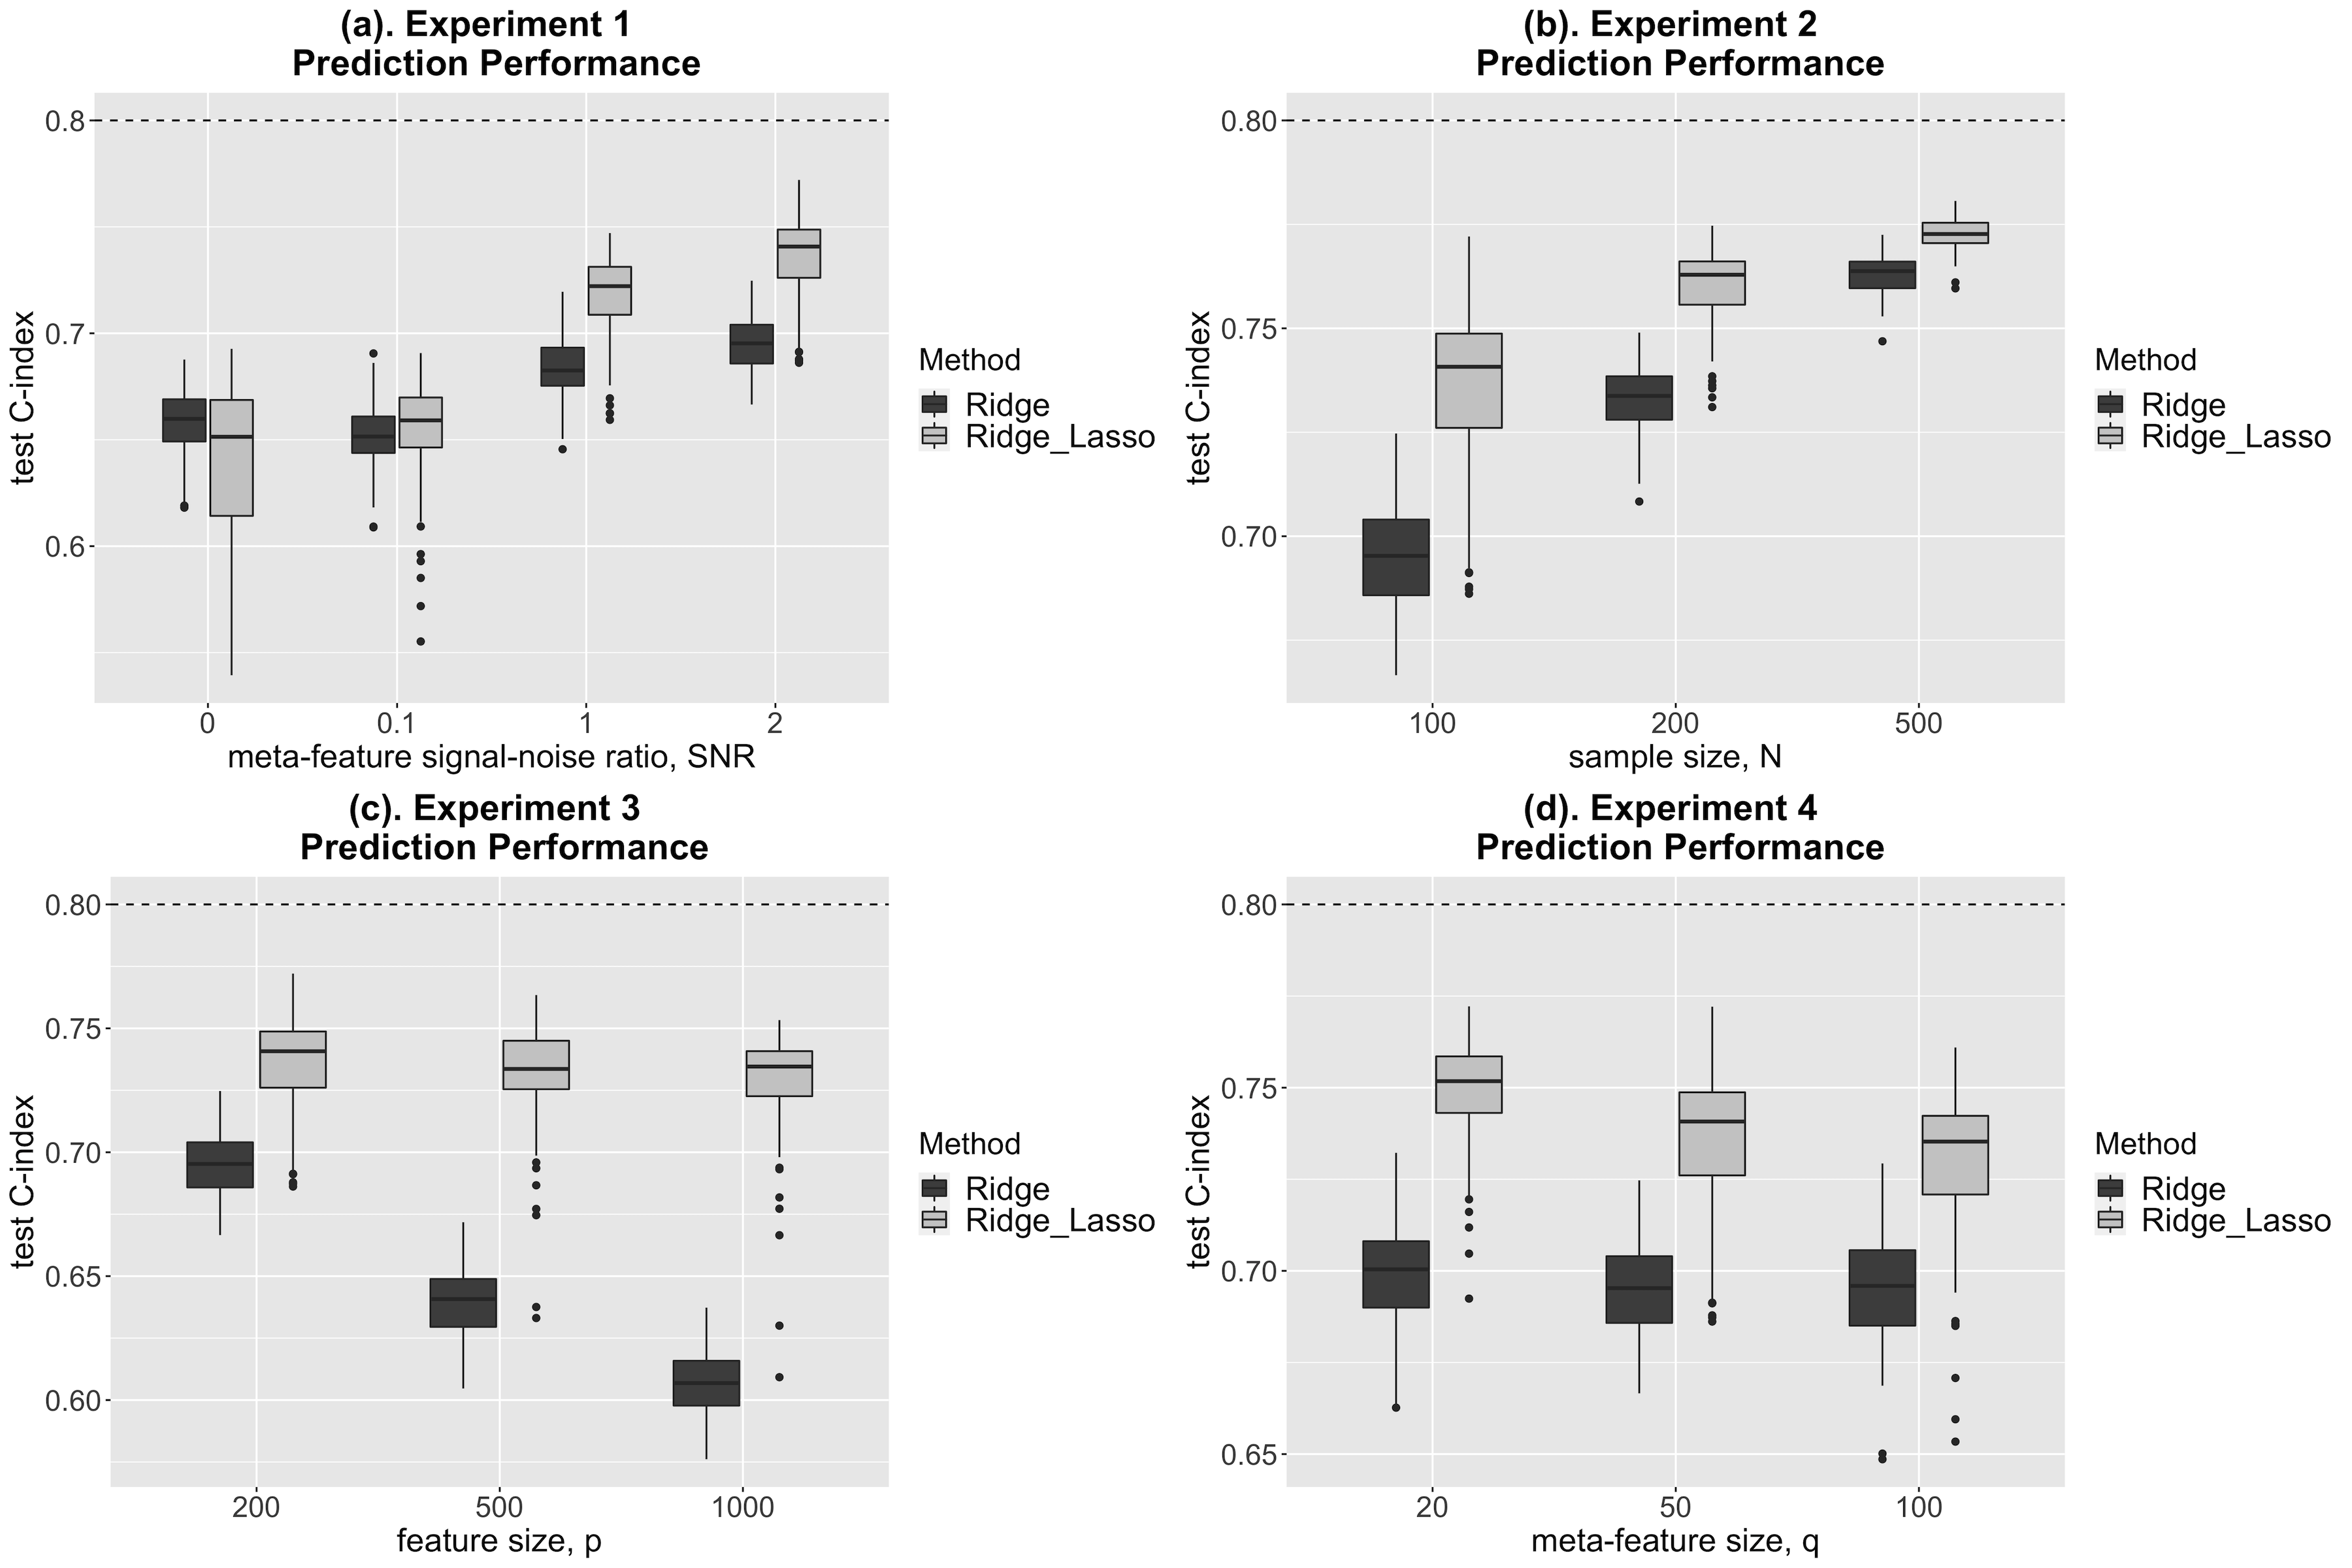
\includegraphics[width=\textwidth]{sim1}
  \caption[Simulation results: prediction performance]{
    Simulation results: prediction performance.
  }
  \label{fig:sim1}
\end{figure}

We also examined the ability of the model to select informative meta-features by second-level Lasso penalty. In particular, we looked at the true and false positive meta-feature selection rate in experiment 1, where the second level meta-features informativeness varies (Figure \ref{fig:sim2}). We see that as the SNR of the meta-features increases, the true positive selection rate of informative meta-features improves dramatically (Figure 2a) at the cost of a slight increase in the false positive rate (Figure 2b).  
\begin{figure}[tbh]
  \centering
  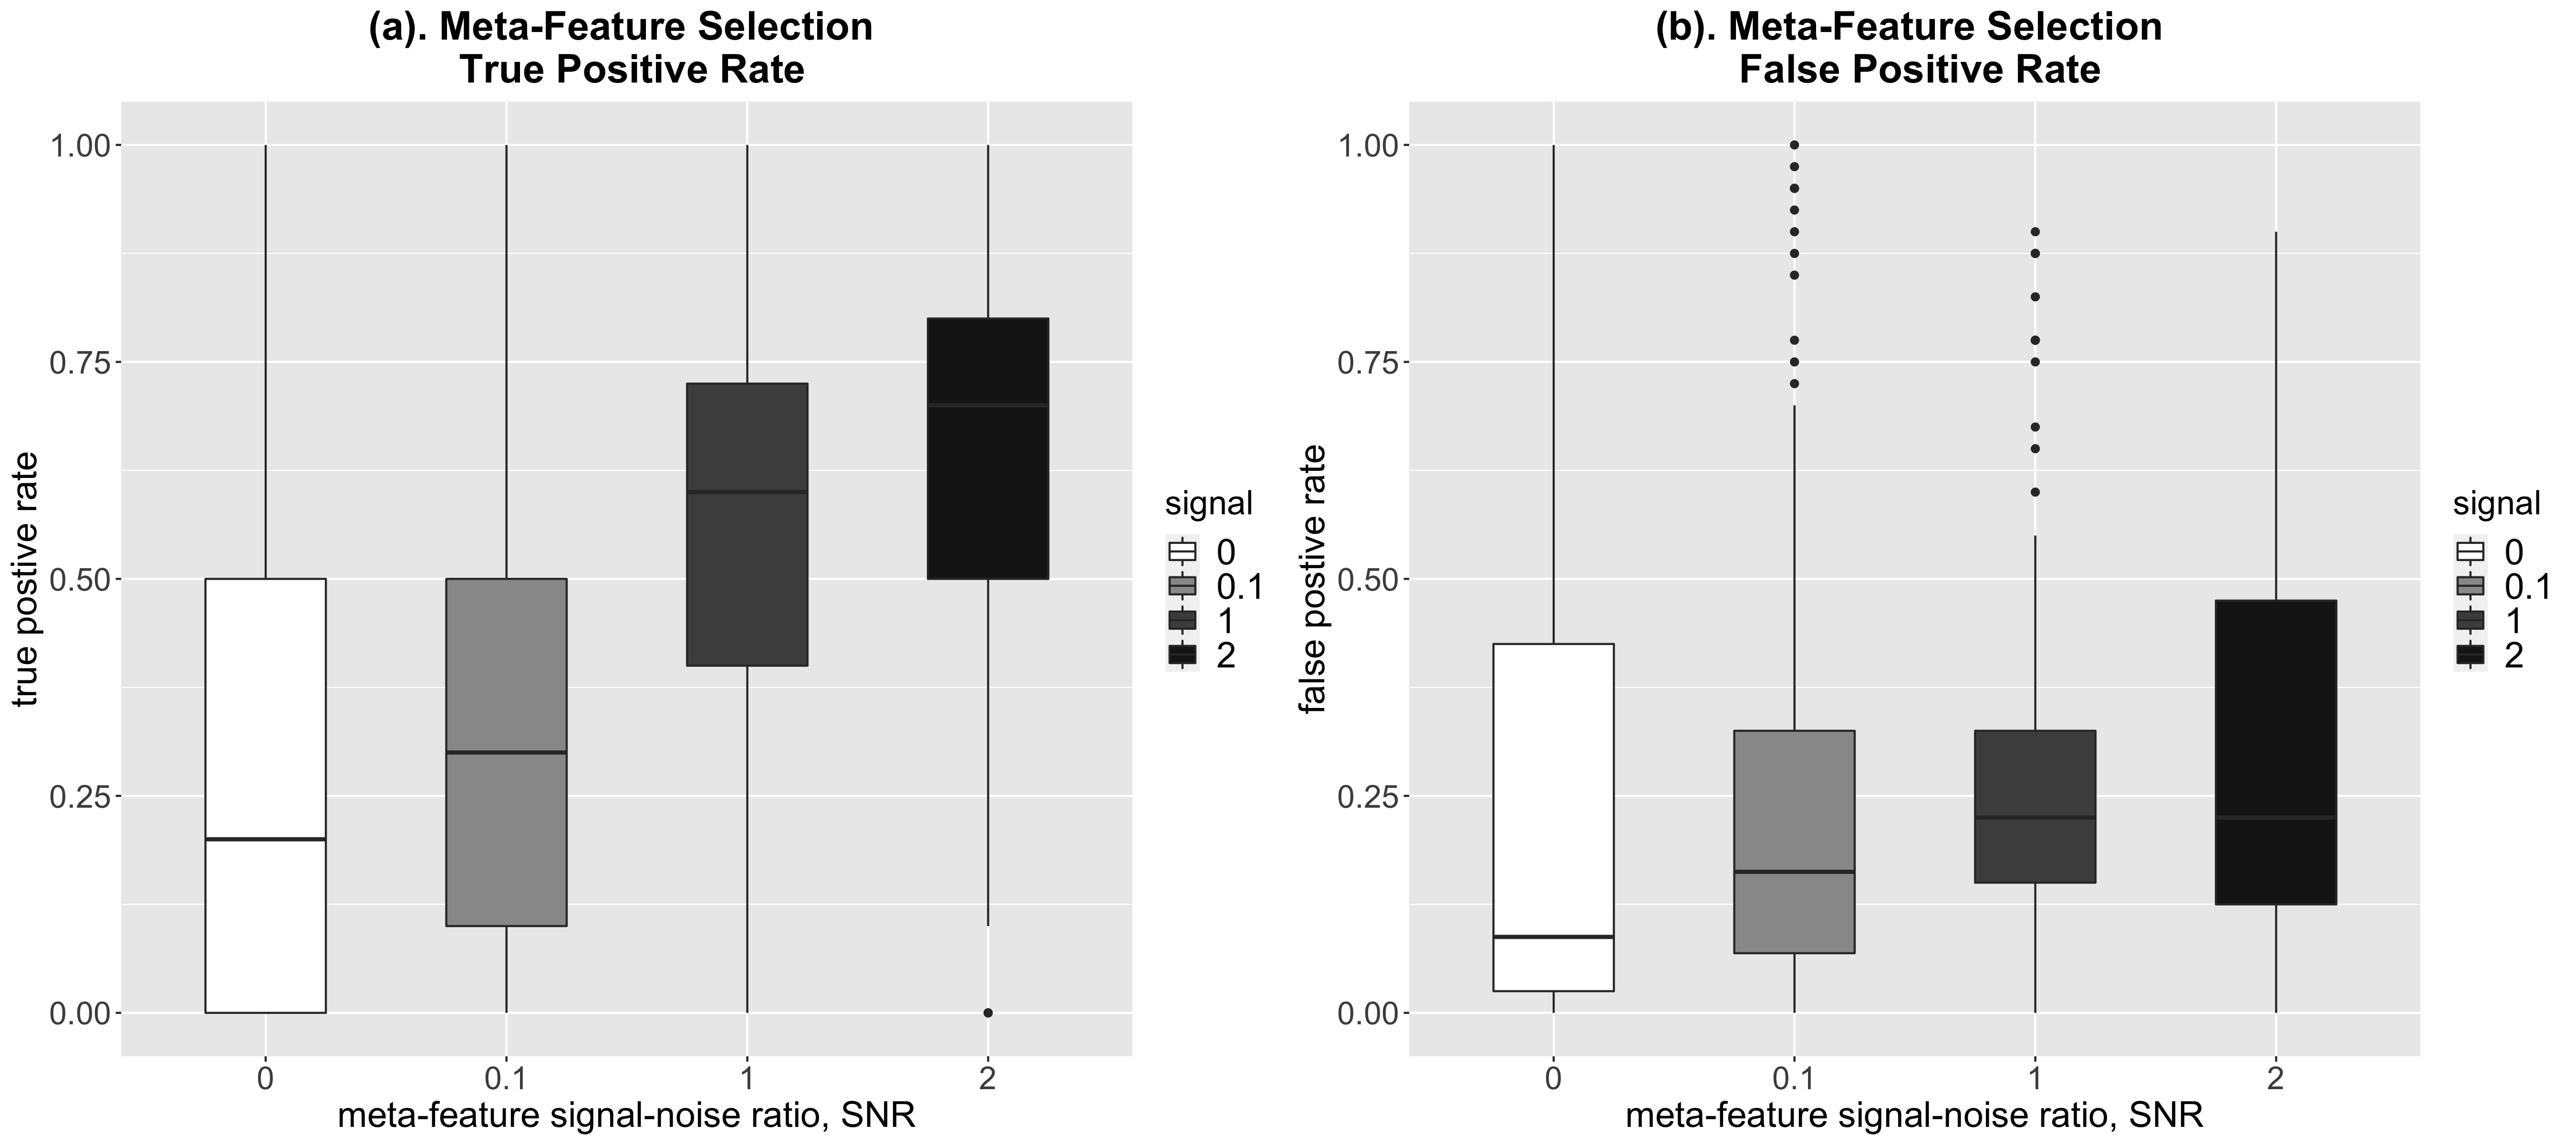
\includegraphics[width=\textwidth]{sim2}
  \caption[Simulation results: meta-feature selection]{
    Simulation results: meta-feature selection.
  }
  \label{fig:sim2}
\end{figure}

\section{Applications}
\subsection{Gene Expression Signatures for Breast Cancer Survival}
To illustrate the performance of our approach, we applied the hierarchical survival model to the Molecular Taxonomy of Breast Cancer International Consortium (METABRIC) study. The METABRIC microarray dataset is available at European Genome-Phenome Archive with the accession of EGAS00000000083. It includes cDNA microarray profiling of around 2000 breast cancer specimens processed on the Illumina HT-12 v3 platform (Illumina\_Human\_WG-v3) \citep{curtis2012genomic}. The dataset was divided into a discovery/training set of 997 samples, and a validation/test set of 995 samples \citep{cheng2013development}. The goal is to build a prognostic model for breast cancer survival, based on gene expressions and clinical features. The data X consists of of 29,477 gene expression probes and two clinical features, age at diagnosis and the number of positive lymph nodes. The meta-feature data $\bm{Z}$ consists of four ``attractor metagenes'', which are selected gene co-expression signatures that are associated with the ability of cancer cells to divide uncontrollably, to invade surrounding tissues, and, with the effort of the organism to fight cancer with a particular immune response \citep{cheng2013biomolecular}. The three universal “attractor metagenes” are genes involved in mitotic chromosomal instability (CIN), in mesenchymal transition (MES), lymphocyte-specific immune recruitment (LYM). In addition, a meta-gene whose expression is associated with good prognosis and that contains the expression values of two genes—FGD3 and SUSD3. The CIN, MES, and LYM metagenes each consist of 100 genes, but for our analysis, we only considered the 50 top-ranked genes. The data matrix $\bm{Z}$ is an indicator matrix of whether a specific expression probe corresponds to a gene in a metagene. 

Model building was based on the samples with ER positive and HER2 negative, as treatments are homogeneous in this group, and they are associated with good prognosis \citep{rivenbark2013molecular}. There were 740 samples in the discovery set and 658 samples in the validation set in the ER+ and HER2- subset after removing samples with missing values. We used 5-fold cross validation to tune the hyper-parameters $\lambda_1,\lambda_2$ in the discovery set. The test set was used to evaluate model performance. The same training/test scheme was used to fit a standard ridge regression without attractor metagene information as comparison. 

With only gene expression features in the model and no clinical features, the test C-index for the ridge-lasso hierarchical model with metagene information was 0.678 which compares favorably with the test C-index of 0.648 for the standard Cox ridge counterpart. When adding the clinical features, age at diagnosis and number of positive lymph nodes, the test C-index increased to 0.752, and 0.727 for the Cox hierarchical model, and the standard Cox ridge model, respectively (Table \ref{table1}). The metagenes``CIN'' and ``FGD3-SUSD3'' were identified by the hierarchical model as being important (had non-zero coefficients). ``CIN'', which is a breast cancer inducing metagene, had a positive coefficient, indicating genes in ``CIN'' had an overall increased risk over other genes, while the ``FGD3-SUSD'' metagene had a negative coefficient estimate, indicating FGD3 and SUSD3 had a reduced risk (Table \ref{table2}). The identified metagenes were also found by previous analysis \citep{cheng2013development}.
\begin{table}[tbh]
    \centering
    \def\arraystretch{1.5}
    \begin{tabular}{|c|c|c|c|}
        \hline
        \multicolumn{2}{|c|}{} & \textbf{Standard Ridge} & \textbf{Ridge-Lasso} \\ 
        \specialrule{.1em}{.05em}{.05em}
        \multirow{2}{*}{\textbf{Test C-index}} & Gene expressions only & 0.648 & 0.678 \\ 
        & Gene expressions + clinical features & 0.727 & 0.752 \\ 
        \hline
    \end{tabular}
    \caption{METABRIC: Test C-index between standard ridge and ridge-lasso}
    \label{table1}
\end{table}

\begin{table}[tbh]
    \centering
    \def\arraystretch{1.5}
    \begin{tabular}{|c|c c|}
        \hline
        \multirow{2}{*}{\textbf{Metagene}} & \multicolumn{2}{ c|}{\textbf{Coefficient Estimate}} \\
         & Gene expressions only & Gene expressions + clinical \\
        \specialrule{.1em}{.05em}{.05em}
        CIN & 0.0094 & 0.0080 \\
        \hline
        MES & 0.0021 & 0.0033 \\
        \hline
        LYM & 0.0011 & 0.0008 \\
        \hline
        FGD3-SUSD3 & -0.2083 & -0.1111 \\
        \hline
    \end{tabular}
    \caption{METABRIC: Coefficient estimates for metagenes}
    \label{table2}
\end{table}

\subsection{Anti-PD1 Immunotherapy Predictive Biomarker for Melanoma Survival}
We also applied the model to a melanoma data set to predict overall survival after treating patients with a PD-1 immune checkpoint blockade. The programmed death 1 pathway (PD-1) is an immune-regulatory mechanism used by cancer to hide from the immune system. Antagonistic antibodies to PD-1 pathway and its ligands, programmed death ligand 1 (PD-L1), has demonstrated high clinical benefit rates and tolerability. Immune checkpoint blockades such as Nivolumab, pembrolizumab are anti-PD-1 antibodies showing improved overall survival for the treatment of advanced melanoma. However, less than 40\% of the patients respond to the treatments \citep{moreno2015anti}. Therefore, predicting treatment outcomes, identifying predictive signals are of great interest to appropriately select patients most likely to benefit from anti-PD-1 treatments. We explored transcriptomes and clinical data using our model to illustrate prediction performance and predictive signal selection.

The dataset combined 3 clinical studies in which RNA-sequencing were applied to patients treated with anti-PD1 antibodies, \cite{gide2019distinct, riaz2017tumor, hugo2016genomic}. The gene expression values are normalized toward all sample average in each study as the control, so that they are comparable to one another across features within a sample and comparable to one another across samples. There are 16010 genes in common across 3 studies and 117 subjects combined. We build predictive models in terms of overall survival, based on gene expression profile. Since the subjects are all treated with anti-PD1 antibodies, the transcriptomic features selected by the model are predictive signals for treatment efficacy or resistance. We selected meta-features from molecular signature database, hallmark gene sets \citep{liberzon2015molecular}. 13 gene sets are enriched to have false positive rates less than 0.25. An indicator matrix $\bm{Z}$ is formed to illustrate whether each of the 16010 genes belong to one of the 13 hallmark gene sets.

We performed 5-fold cross validation to tune the hyperparameters and report the validation prediction performance. We see an improvement in prediction with the hallmark gene set information with a C-index of 0.663 for ridge-lasso compared to 0.637 for standard ridge. At the gene set level, among model selected sets (non-zero coefficient $\alpha$), 3 gene sets have absolute effect size larger than 0.01 (Table \ref{table3}). Specifically, genes in response to interferon gamma, genes that are involved in KRAS regulation were identified. A subset of the genes in the identified gene sets by our model were in concordance with the previously published anti-PD1 gene signatures \citep{riaz2017tumor, hugo2016genomic}.
\begin{table}[tbh]
    \centering
    \def\arraystretch{1.3}
    \begin{tabular}{|c|c|}
        \hline
        \textbf{Gene set} & \textbf{Coefficient estimate}  \\
        \specialrule{.1em}{.05em}{.05em}
        IFNG interferon gamma response & -0.0100* \\
        Interferon alpha response & -0.0013 \\
        IL-2\_STAT5 signaling & 0.0072 \\
        Bile acid metabolism & -0.0011 \\
        KRAS signaling down regulated & -0.0135* \\
        KRAS signaling up regulated & 0.0100* \\
        Apoptosis & 0.0004 \\
        Xenobiotic metabolism  & 0.0013 \\
        \hline
    \end{tabular}
    \caption[Coefficient estimates (nonzero) for meta-features]{
        Coefficient estimates (nonzero) for meta-features. * Gene sets with absolute value of coefficients larger than 0.01.
        }
    \label{table3}
\end{table}

\section{Discussion}
In this paper we extended the regularized hierarchical regression model of [Lee. et. al] to time-to-event data and to accommodate a lasso or elastic-net penalty in the second-level model. The hierarchical regularized regression model enables integration of external meta-feature information directly into the modeling process.  We showed that prediction performance improves when the external meta-feature data is informative. And the improvements are largest for smaller sample sizes, when prediction is hardest and performance improvement is most needed. Key to obtaining performance gains though is prior knowledge of external information that is potentially informative for the outcome. For example, clinicians, epidemiologists, or other substantive experts may provide insights into what type of annotations are likely to be informative.  However, the model is robust to incorporating a set of meta-features that is completely irrelevant to the outcome of interest.  In this scenario, a very small price in prediction performance is paid relative to a standard ridge model (i.e., without external information). This should encourage the user to integrate meta-features even if uncertain about their informativeness.

An underlying assumption of the proposed regularized hierarchical model is that the effects in a group determined by meta-features (e.g., genes in a pathway) are mostly in the same direction. A limitation of the method is that if the effects have opposite signs and ‘cancel each other out’ there would be little or no improvement in prediction, even if the pathway information is informative.

In addition to developing predictive signatures, the model can also be deployed in discovery applications where the main goal is to identify important features associated with the outcome rather than developing a predictive model. However, there is no standard way to perform formal inference (standard errors, p-values, confidence intervals) with high-dimensional regression models. Several approaches exist \citep{meinshausen2009p, shah2013variable} and this is an active area of research. Adding formal statistical inference would be an important future work to expand the range of use of the proposed model. 

The regularized hierarchical model is implemented in the``xrnet'' R package available from CRAN. The implementation is efficient and can be used to perform analyses with large numbers of features, meta-features, and subjects. While the models we focused on in the simulation and data applications are all “ridge-lasso”, i.e., with an $L_2$ norm penalty applied to $\bm{\beta}-\bm{Z\alpha}$, and an $L_1$ norm applied to the meta-feature coefficients $\bm{\alpha}$, the package offers the flexibility of using the Lasso, elastic net, and ridge penalties to penalize the meta-features depending on the application.  For example, if selection at the meta-feature level is desired and the meta-features are highly correlated, the elastic net penalty is a better option for $\bm{\alpha}$ regularization. Because if there is a group of variables that are highly correlated, the lasso tends to select one of them, while the elastic net enjoys grouping effect which selects all the variables in a group with estimated coefficients close to equal in magnitude \citep{zou2005regularization}. The approach does not perform feature selection on first level information as it uses a ridge penalty. In a high dimensional setting, standard regularized regression like lasso and elastic net often select relatively large numbers of features. It can then be valuable to identify groups of genes defined by meta-features that may jointly have significant predictive power for the outcome of interest. Another potential improvement of the model is to extend the range of penalty types to nonconvex penalties, such as SCAD \citep{fan2001variable}, MCP \citep{zhang2010nearly}. These penalties yield less biased effect size estimates than that of lasso and elastic net.



% Research Topic 2
\chapter{Genomic Meta-Feature Guided Regularized Regression for Survival Outcome}
\label{cha:xtunecox}

\section{Abstract}
In building predictive models for genomic studies, regularized regression is a common technique as the number of genomic features is much larger than the number of samples. The application of sparse regularized regression performs feature selection while doing prediction. Associated with genomic features, such as gene expression, genetic variation, DNA methylation, there are plenty of meta-features. Some examples are functional gene sets, gene ontology annotations, knowledge of past studies. Existing method is to model genomic features on phenotypic outcomes, and post hoc analysis with meta-features, like gene set enrichment analysis. However, incorporating meta-features into modeling process can potentially improve the quality of both prediction performance and feature selection. 

In this paper, we extend the approach of \cite{zeng2021incorporating} to survival outcome. The method incorporates genomic meta-features to guide the regularized Cox regression, so that each of the genomic features has its own customized penalty parameter, as opposed to one common penalty parameter for all features. With highly informative meta-features, significant features become more important/being penalized less, unrelated features become less important/heavily penalized, thereby achieving improved feature selection. The prediction performance is also improved with the extra meta-feature information. We show the benefits of the method by simulations and applications in genomic studies. Model optimization algorithm involves empirical Bayes estimation of penalty parameters, and a majorization-minimization procedure. 

\section{Introduction}
Predicting a phenotypic outcome based on genomic features is a highly active research area, with the increasing need in personalized health care to achieve the best outcome for individual patients. A common technique for genomic predictive modeling is regularized regression. As the number of genomic features is typically large, thousands to millions, linear models like regression are better suited. Because the data pattern is most likely linear where each feature contribute a little or none effect to the outcome. When number of features is larger than the number of samples, which is usually the case for genomics study, regularization needs to be introduced so that the model can be fit. Sparse regularized regression is a popular choice, as it not only shrinks the regression coefficients to make the model simpler, it also shrink some of the coefficients with little effects on the outcome to exactly zero, thereby performing feature selection. Typical examples are the lasso \citep{tibshirani1996regression} and the elastic net \citep{zou2005regularization}. While they have similar mechanics, there is a major difference. If some of the features among which the correlations with each other are high, the lasso tends to select one of them, while the elastic net tends to select most of them and share the lasso value equally. Ridge regression \citep{hoerl1970ridge} is another regularization technique to cope with high dimension and collinearity of data. However, it only shrinks the coefficients, not to zero, hence does not produce interpretable model. 

Genomic features may have their own characteristics: grouping effect and ordering. Extensions of the lasso deal with such situations. The group lasso \citep{yuan2006model} takes in the grouping information, shrinking coefficients by group. All the coefficients in one group are either zero or nonzero. Sparse group lasso \citep{simon2013sparse} further allows sparsity within group. The fused lasso deals with the ordering situation, with the addition of $L_1$ terms for the differences of neighbouring coefficients, which allows sparsity in their differences. The above extended regularization methods take into account characteristics of features, which are essentially features of the features if they are put in a data set. We call these underlying characteristics of features "meta-features" here and after. There are plenty of such meta-features in genomics. For example, functional gene sets like hallmark \citep{liberzon2015molecular}, gene ontology pathways like reactome \citep{jassal2020reactome} work as grouping effect; summary statistics like p-values and regression coefficients from meta-analyses work as ordering effect (p-values and regression coefficients indicate the importance of each feature). The meta-features are actual data matrices, where the samples/rows represent original features, and the columns represent meta-features. However, none of the above regularization approaches systematically utilize the meta-feature information. The group lasso assumes features are in different groups mutually exclusive. Features in multiple groups at the same time does not meet the assumption. The fused lasso takes the ordering of the features into account, but when provided with concrete information like p-values indicating exactly how important each feature are, it cannot incorporate such information. 

One way of utilizing the meta-features is modeling with original features, and performing gene set enrichment analysis \citep{subramanian2005gene} post hoc. However, incorporating meta-features into modeling process can potentially improve both prediction performance and the quality of feature selection. Weaver et al. (reference) and Shen et al. (reference) incorporate the meta-features in a hierarchical modeling setup. The outcomes are regressed on original features, assuming quantitative outcome, 
$$ \bm{Y} = \bm{X\beta} + \bm{\varepsilon} $$ 
where $\bm{Y}$ is the length $n$ outcome vector, $\bm{X}$ is the $n \times p$ data matrix, $\bm{\beta}$ is the length $p$ feature coefficient vector to be estimated in the model. Then the feature coefficients $\bm{\beta}$ are regressed on meta-features,
$$ \bm{\beta} = \bm{Z\alpha} + \bm{\gamma} $$
where $\bm{Z}$ is the $p \times q$ meta-feature matrix, $\bm{\alpha}$ is coefficients vector for meta-features. To integrate both level of features into modeling process, an objective function is formed as below 
$$ \min_{\bm{\beta, \alpha}} \frac{1}{2n} \|\bm{Y}-\bm{X \beta} \|_2^2 + \frac{\lambda_1}{2} \|\bm{\beta} - \bm{Z \alpha} \|_2^2 + \lambda_2 \|\bm{\alpha}\|_1 $$
The original feature data $\bm{X}$ and meta-feature data $\bm{Z}$ are fitted through two least squares. The additional $L_1$ term of meta-feature coefficients $\bm{\alpha}$ is to control model complexity and meta-feature selection. This integration method incorporates meta-features linearly, emphasizing on meta-feature selection. It was shown to improve the prediction performance considerably with high quality meta-features. \cite{zeng2021incorporating} developed another method for integrating meta-features $\bm{Z}$ for quantitative and binary outcomes, in a non-linear way, such that each of the original features has its own customized penalty parameter, as opposed to one common penalty parameter for all features. The customized penalty parameters potentially allow more accurate feature selection. In this paper, we extend this approach to survival outcomes. 

\section{Methods}
\subsection{Model setup and notations}
Starting with the survival model setup, let the outcome data be $(\bm{y, \delta})$ where $\bm{y}=(y_1,y_2,\dots,y_n)$ is observed time, $\delta=(\delta_1,\delta_2,\dots,\delta_2)$ is censoring status. If $\delta_i = 1 (i=1,2,\dots,n)$, event happened, $y_i$ is event time; if $\delta_i=0$, event did not happen in experimental period, $y_i$ is censoring time. There are $p$ features for the n instances/samples, data matrix $\bm{X}$ with dimension $n\times p$ stores the feature values, i.e., $\bm{x}_i$ is a vector of feature values for instance $i$ $(x_{i1},x_{i2},\dots,x_{ip})$. Associated with the features, there are q meta-features. A $p\times q$ matrix $\bm{Z}$ stores the meta-feature values for the $p$ original features, i.e., $\bm{z}_j (j=1,2,\dots,p)$ is a vector of meta-feature values for feature $j$ $(z_{j1},z_{j2},\dots,z_{jq})$. The common choice of regression method is Cox's proportional hazards model \citep{cox1972regression}. It assumes hazard functions are proportional at the same time point, which allows model fitting without knowing explicit form of baseline hazard function, and only depends on the order in which events occur, not on the exact time of occurrence. To illustrate, let $t_1<t_2<\dots<t_l<\dots<t_m$ be the the unique event times arranged in increasing order, and $D_l=\{i:\delta_i=1,y_i=t_l\}$ is the set of instances experienced event at time $t_l$. Let $\bm{\beta}$ be a length $p$ vector for the feature regression coefficients. The partial likelihood function, $L(\bm{\beta})$, takes the form 
\begin{displaymath}
L(\bm{\beta}) = \prod_{l=1}^{m} \frac{e^{\sum_{i\in D_l}\bm{x}_i^T\bm{\beta}}}{(\sum_{i\in R_l} e^{\bm{x}_i^T\bm{\beta}})^{d_l}}
\end{displaymath}
where $R_l=\{i: y_i\geq t_l\}$ is the risk set at event time $t_l$, i.e., the set of all instances who have not experienced the event and are uncensored just prior to time $t_l$; $d_l=|D_l|$ is the number of events at time $t_l$. $L(\bm{\beta})$ is Breslow's adjustment of partial likelihood \citep{breslow1972contribution}. It deals with ties in each event time ($d_l>1$: more than one instance experienced event at a particular event time). When there are no ties ($d_l=1$), $L(\bm{\beta})$ automatically reduces to Cox's partial likelihood. We can see that neither hazard functions nor times are involved in the function, only the order of event times matters. 

We add regularization to Cox regression to control model complexity. Denote the log of partial likelihood as $\ell(\bm{\beta})$,
\begin{equation} \label{eq1}
    \min_{\bm{\beta}\in \mathbb{R}^p} \left\{-\ell(\bm{\beta}) + \lambda\left[\frac{1}{2}(1-c)\|\bm{\beta}\|_2^2 + c\|\bm{\beta}\|_1\right]\right\}.
\end{equation}
The regularization function covers lasso, elastic net, ridge penalties, i.e., $c=1$ represents the lasso, $c=0$ represents ridge, and $0<c<1$ represents the elastic net. When $0<c\leq1$, it is sparse regularization which shrink some coefficients to exactly zero, producing interpretale model. The regularization has a universal penalty parameter $\lambda$ for all the features. This ignores underlying characteristics of features assuming each of them are equally important by applying the same amount of penalty. Our idea is to incorporate informative meta-features which might indicate the importance of the original features, giving each of them a unique penalty parameter $\lambda_j$. To incorporate meta-features to $\lambda_j$, first form a linear combination of $\bm{z_j}$ for feature $j$, $\bm{\alpha}$ is the weight vector of length $q$; then give it a non-linear function by expenentiating it
\begin{equation} \label{eq2}
\begin{aligned}
    &\min_{\bm{\beta}\in \mathbb{R}^p} \left\{-\ell(\bm{\beta}) + \sum_{j=1}^p \lambda_j\left[\frac{1}{2}(1-c)\beta_j^2 + c|\beta_j|\right]\right\}, \\
    &\lambda_j = e^{\bm{z_j}^T \bm{\alpha}}.
\end{aligned}
\end{equation}

\subsection{Model fitting}
The standard regularized Cox proportional hazards model, equation \eqref{eq1}, is fitted with pathwise coordinate descent \citep{simon2011regularization}. As the universal penalty parameter $\lambda$ is a hyper-parameter, the algorithm constructs a $\lambda$ path to tune via cross-validation. The proposed model, equation \eqref{eq2}, has $p$ $\lambda$'s decided by weights $\bm{\alpha}$, $\bm{\lambda} = (\lambda_1,\lambda_2,\dots,\lambda_p) = e^{\bm{Z\alpha}}$, it is impossible to tune them. Instead, we estimate the weights $\bm{\alpha}$ first to get the values of $\bm{\lambda}$. With known $\bm{\lambda}$, we can fit the model via coordinate descent.

\subsubsection{Empirical Bayes estimation of hyperparameter} \label{laplace}
To estimate $\bm{\alpha}$, we need to form an objective function. Since the regularized regression has a natural Bayesian  interpretation, we apply empirical Bayes estimation of hyper-parameters in random effects model, which is maximizing marginal likelihood in terms of hyper-parameter $\bm{\alpha}$ obtained by integrating out random effects $\bm{\beta}$. Based on the Bayesian elsatic net \citep{li2010bayesian}, equation \eqref{eq2} has the interpretation
\begin{align}
    &f(\bm{Y}|\bm{\beta}; \bm{X}) = L(\bm{\beta}) \label{eq3}, \\
    &\pi(\beta_j; \bm{\alpha}) \propto exp\left\{ -\lambda_j\left[\frac{1}{2}(1-c)\beta_j^2 + c|\beta_j|\right] \right\}. \label{eq4}
\end{align}
With the likelihood \eqref{eq3} and prior distribution \eqref{eq4}, we construct the joint distribution of $\bm{Y}$ and $\bm{\beta}$, and integrate out $\bm{\beta}$, so to get the marginal likelihood of $\bm{Y}$,
\begin{align*}
\ln f(\bm{Y};\bm{\alpha}) &= \int_{\bm{\beta}\in\mathbb{R}^p} \ln f(\bm{Y}, \bm{\beta};\bm{\alpha}) d\bm{\beta} \\
&= \int_{\bm{\beta}\in\mathbb{R}^p} \left[\ln f(\bm{Y}|\bm{\beta};\bm{X})+\ln \pi(\bm{\beta};\bm{\alpha})\right]d\bm{\beta} \\
&= \int_{\bm{\beta}\in\mathbb{R}^p} \left\{ \sum_{l=1}^{m}\left[\sum_{i\in D_l}\bm{x}_i^T\bm{\beta}-d_l\ln(\sum_{i\in R_l} e^{\bm{x}_i^T\bm{\beta}})\right] - \sum_{j=1}^{p} \lambda_j\left[\frac{1}{2}(1-c)\beta_j^2 + c|\beta_j|\right]+ \text{const} \right\} d\bm{\beta}
\end{align*} 
This integral does not have a closed form expression because the elastic net prior is not a conjugate prior for the likelihood. We propose two approximation procedures: first approximate the elastic net prior to a normal prior, then apply Laplace approximation. To approximate the elastic net prior, we follow Zeng et al. (2021) (reference),  
\begin{equation}
    \pi(\beta_j; \bm{\alpha}) = N(0, \frac{2}{2\lambda_j(1-c)+c^2\lambda_j^2}). \label{eq5}
\end{equation}
Equation \eqref{eq5} gives a similar variance to that of the elastic net prior. The joint distribution, $\ln f(\bm{Y}, \bm{\beta};\bm{\alpha})$, then takes the form 
\begin{equation} \label{eq6}
\begin{aligned}
    &\ln f(\bm{Y}, \bm{\beta};\bm{\alpha}) = \sum_{l=1}^{m}\left[\sum_{i\in D_l}\bm{x}_i^T\bm{\beta}-d_l\ln(\sum_{i\in R_l} e^{\bm{x}_i^T\bm{\beta}})\right] - \sum_{j=1}^{p} \frac{1}{2}v_j\beta_j^2 + \text{const}, \\
    &v_j = \frac{2\lambda_j(1-c)+c^2\lambda_j^2}{2}.
\end{aligned}
\end{equation}
This is essentially a ridge regularized Cox regression with customized penalty vector. 
For Laplace approximation of the marginal likelihood/model evidence, we elaborate the details. Consider a Taylor series of $\ln f(\bm{Y}, \bm{\beta};\bm{\alpha})$ at the stationary point $\widetilde{\bm{\beta}}$, where $\nabla \ln f(\bm{Y}, \widetilde{\bm{\beta}};\bm{\alpha})=0$,
$$ \ln f(\bm{Y}, \bm{\beta};\bm{\alpha}) \approx \ln f(\bm{Y}, \widetilde{\bm{\beta}};\bm{\alpha}) - \frac{1}{2}(\bm{\beta}-\widetilde{\bm{\beta}})^T\bm{H}(\bm{\beta}-\widetilde{\bm{\beta}}). $$
$\widetilde{\bm{\beta}}$ is the solution of a ridge regularized Cox regression as already stated, it can be computed using \textbf{R} language \emph{glmnet} package \citep{simon2011regularization}, with known $\bm{\alpha}$. $\bm{H}$ is the Hessian matrix,
\begin{align*}
    \bm{H} &= - \nabla\nabla \ln f(\bm{Y}, \bm{\beta};\bm{\alpha})|_{\bm{\beta}=\widetilde{\bm{\beta}}} \\
    & \approx \bm{X}^T\bm{W}\bm{X} + \bm{V}
\end{align*}
where $\bm{V} = \text{diag}[\bm{v}]=\text{diag}[v_1,\dots,v_p]$, $\bm{W}$ is a diagonal matrix with elements 
$$ \bm{W}_{ii} = \sum_{l\in C_i}\frac{d_le^{\bm{x}_i^T\bm{\beta}}}{\sum_{k\in R_l}e^{\bm{x}_k^T\bm{\beta}}} - \sum_{l\in C_i}\frac{d_l(e^{\bm{x}_i^T\bm{\beta}})^2}{(\sum_{k\in R_l}e^{\bm{x}_k^T\bm{\beta}})^2}. $$ 
The Hessian is an approximation because $W$ is in fact a full matrix with high computational cost. We only use diagonal elements to speed up computation without much loss of accuracy. For greater details, refer to Shen et al. (2021) (reference).
Now that we see $f(\bm{Y}, \bm{\beta};\bm{\alpha})$'s Taylor approximation has a multivariate normal form with mean $\widetilde{\bm{\beta}}$, variance $\bm{H}^{-1}$, integrating out $\bm{\beta}$ returns the normalizing constant.
\begin{equation} \label{eq7}
\begin{aligned}
    -\ln{f(\bm{Y};\bm{\alpha})} &\approx -\ln f(\bm{Y}|\widetilde{\bm{\beta}};\bm{X}) - \ln \pi(\widetilde{\bm{\beta}};\bm{\alpha}) - \frac{p}{2}\ln{2\pi} + \frac{1}{2}\ln{|\bm{H}|} \\
    &= -\ln{|\bm{V}|} + \widetilde{\bm{\beta}}^T\bm{V}\widetilde{\bm{\beta}} + \ln{|\bm{H}|} + \text{const}
\end{aligned}
\end{equation}
The approximate negative log marginal likelihood, equation \eqref{eq7}, is the objective function we are going to minimize with respect to $\bm{\alpha}$.

\subsubsection{Objective function optimization} \label{DCA}
The objective function, equation \eqref{eq7}, is nonconvex. In particular, it can be decomposed as difference of two convex functions. $g(\bm{\alpha}):=-\ln{|\bm{V}|} + \widetilde{\beta_j}^T\bm{V}\widetilde{\beta_j}$ is convex in $\bm{\alpha}$, whereas $h(\bm{\alpha}):=\ln{|\bm{H}|}$ is concave. This makes it a proper candidate to apply difference of convex functions algorithm (DCA) \citep{le2015dc}. The principle idea of DCA is to approximate the nonconvex objective function by a sequence of convex ones: at each iteration of the sequence, approximate the concave part by its affine majorization, i.e., the supporting hyperplane obtained by calculating its gradient, or subgradients if not differentiable, and minimize the resulting convex approximation. Note that it is also an application of majorization-minimization algorithm \citep{hunter2004tutorial}. The affine approximation of the concave part is the majorization step, which forms a surface lying above the objective function, and is tangent to it, i.e, at the current estimation of the target parameter, the majorization equals to the objective function. This ensures the majorization is a tight upperbound for the objective. Minimizing the convex upperbound is the minimization step. The DCA algorithm for the marginal likelihood, $-\ln{f(\bm{Y};\bm{\alpha})}$:
\begin{enumerate}
    \item Initialize $\bm{\alpha}$ with $\widetilde{\bm{\alpha}} \in \mathbb{R}^q$.
    \item Majorization: 
    \begin{itemize}
        \item calculate the gradient at current estimation $\widetilde{\bm{\alpha}}$,
    $$\bm{\theta}= \nabla_{\bm{v}} \ln{|\bm{H}|} = \text{diag}[\bm{H}^{-1}]$$ 
        \item form the convex upperbound,
        \begin{align*}
        u(\bm{\alpha})&=g(\bm{\alpha})+ h(\widetilde{\bm{\alpha}}) + \bm{\theta}^T(\bm{v}-\widetilde{\bm{v}}) \\
        &=-\ln{|\bm{V}|} + \widetilde{\bm{\beta}}^T\bm{V}\widetilde{\bm{\beta}}+\bm{\theta}^T\bm{v}+\text{const}
        \end{align*}
    \end{itemize}
    \item Minimization: $\hat{\bm{\alpha}}=\underset{\bm{\alpha}}{\operatorname{\argmin}} \left\{u(\bm{\alpha})\right\}$.
    \item Set $\widetilde{\bm{\alpha}} = \hat{\bm{\alpha}}$.
    \item Repeat step 2-4 until convergence of $\hat{\bm{\alpha}}$.
\end{enumerate}
The minimization of $u(\bm{\alpha})$ can be processed with standard first order method like gradient descent, or second order method like Newton-Raphson. We show the gradient and Hessian here,
\begin{align*}
    &\nabla_{\bm{\alpha}} u(\bm{\alpha}) = \bm{Z}^T\left[(-\frac{1}{\bm{v}}+\widetilde{\bm{\beta}}^2+\bm{\theta})((1-c)\bm{\lambda}+c^2\bm{\lambda}^2)\right],\\
    &\nabla\nabla_{\bm{\alpha}} u(\bm{\alpha}) = \bm{Z}^T \text{diag}\left[\frac{\bm{\lambda}^2}{\bm{v}^2}(1-c+c^2\bm{\lambda})^2+(-\frac{1}{\bm{v}}+\widetilde{\bm{\beta}}^2+\bm{\theta})\bm{\lambda}(1-c+2c^2\bm{\lambda})\right]\bm{Z}.
\end{align*}

\subsection{Summary}
We incorporate the meta-features into the penalty parameter of regularized Cox proportional hazards model, as a log-linear function, to give each feature a unique penalty parameter depending on the meta-features. We then apply Bayesian interpretation of regularized regression to obtain the marginal likelihood function, as the objective function to optimize with respect to the introduced meta-feature weights $\bm{\alpha}$, thereby estimating the customized penalty parameter vector $\bm{\lambda}$. The nonconvex objective function can be decomposed to a difference of two convex functions, which can be solved with difference of convex functions algorithm. With estimated $\bm{\alpha}$, we can plug values of penalty parameters into the regularized Cox regression. The model fitting procedure is
\begin{enumerate}
    \item Initialize $\bm{\alpha}$ with $\widetilde{\bm{\alpha}}$.
    \item Repeat, until convergence of $\hat{\bm{\alpha}}$.
    \begin{enumerate}
        \item Laplace approximation of marginal likelihood with known $\widetilde{\bm{\alpha}}$, section \ref{laplace},
        \begin{itemize}
            \item Approximate the elastic net prior with a normal prior, equation \eqref{eq6},
            \item Calculate $\widetilde{\bm{\beta}}$ and $\bm{H}$.
        \end{itemize}
        \item Optimize Laplace approximation of marginal likelihood, equation \eqref{eq7}, get solution $\hat{\bm{\alpha}}$, with DCA described in section \ref{DCA}.
        \item Set $\widetilde{\bm{\alpha}} = \hat{\bm{\alpha}}$.
    \end{enumerate}
    \item Calculate customized penalty vector $\bm{\lambda}=e^{\bm{Z}\hat{\bm{\alpha}}}$.
    \item Fit regularized Cox regression, equation \eqref{eq2}, with $\bm{\lambda}$.
    
\end{enumerate}

\section{Simulations}
\subsection{Simulation methods}
In this section, we perform simulations to evaluate the model performance. The purpose of the simulation is to compare prediction, feature selection between our proposed model and standard regularized Cox regression. We generate meta-feature data $\bm{Z}$ from independent Bernoulli variables, with probability 0.1. This is to simulate biological pathway/functional gene set meta-features. Each pathway contains a group of genes, 1 indicates the gene being in the pathway group, 0 otherwise. Meta-feature weights $\bm{\alpha}$ are set to be fixed, values are from -1 to 1 equally spaced. We then can generate $\bm{\beta}$ from its normal prior distribution with mean 0, variance computed from $\bm{\alpha, Z}$, equation \eqref{eq5}. Note that we want the underlying model to be sparse, so we keep the top 20\% of the $\bm{\beta}$ elements with largest absolute values, and set the remaining to be 0. In this step, we can control the informativeness of the meta-features. Once $\bm{\beta}$ are generated, meta-features are fully informative to the model. We randomly change some of the rows of $\bm{Z}$ to opposite values (0 to 1, 1 to 0) so that the proportion of rows modified indicates the informativeness of meta-features, i.e., 10\% of the rows modified shows high informativeness while 90\% of the rows modified indicates low informativeness. Data matrix $\bm{X}$ are distributed as a multivariate normal with an autoregressive correlation structure, $\bm{\Sigma}_{ij} = \rho^{|i-j|}$, set $\rho=0.5$. Survival times are generated based on inverse probability integral transform,   
\begin{displaymath}
t = H_0^{-1}\left(-\ln(U)e^{-\bm{\beta}^T\bm{x}}\right)
\end{displaymath}
where $U\sim \text{uniform}[0,1]$, $H_0(t) = (t/5)^8$ is the baseline cumulative hazard function with Weibull distribution. Censoring time is from an exponential distribution, $c\sim \text{exp}(0.1)$. The distribution parameter values set for Weibull and exponential are to produce survival times range from 0 to 20, and a fixed ratio of events to censoring. We then add a normal noise to survival times to fix the model underlying predictive ability at concordance measure \citep{harrell1982evaluating} 0.8, by controlling the standard deviation of the noise. The survival time outcome is set to be the minimum of survival and censoring time, $y=\text{min}(t,c)$. And it is said to be censored $\delta=0$ if $c<t$, the observation loses follow up before event happens. 

For each simulation, we generate data as described above. We fit standard elastic net regularized Cox regression without external meta-features $\bm{Z}$, and also fit our proposed model with meta-features. Elastic net regression is tuned with 5-fold cross validation, while the proposed model does not require penalty parameter tuning as it is estimated during model fitting procedure. We then compare the prediction performance between the two models on simulated test set. The simulation steps are performed with 100 replicates. 

We run a series of experiments varying one key parameter while keeping the others fixed. The base case parameters are sample size $n=100$, feature size $p=200$, meta-feature size $q=10$, meta-feature $\bm{Z}$ informativeness: 5\% of features (rows of $\bm{Z}$) has been modified to have incorrect values. This is a high informativeness level. 4 experiments are conducted by varying one parameter at a time.
\begin{enumerate}
    \item Meta-feature informativeness level from high to low, proportion of rows of $\bm{Z}$ modified 5\%, 15\%, 30\%.
    \item Feature size, $p=200, 600, 1000$.
    \item Sample size, $n=100, 200, 300$.
    \item Meta-feature size, $q=10, 20, 30$.
\end{enumerate}
In experiment 1, we also examined quality of feature selection by both models, to evaluate how informativeness of meta-features influences model interpretation.

\subsection{Simulation results}
Figure \ref{fig:sim21} shows the results of 4 simulation experiments. The horizontal dashed line in each panel represents the population/theoretical C-index, achievable with infinite samples of training data. It is provided as a reference for each parameter setting. The performance of meta-feature guided elastic net Cox model (denoted as `meta' in the figure) is compared to that of a standard elastic net Cox model. 

In experiment 1, there are consistent improvements in prediction performances as long as the meta-features are informative. The higher the informativeness of meta-features, the more improvements gained in prediction performance over the standard elastic net model. In the figure, the difference of test C-index between the two models increases with the informativeness of meta-features. 

Experiment 2 illustrates model performances with respect to feature size. Larger number of features relative to sample size makes it harder for both models to predict, as both models' test C-indexes are way below the theoretical C-index, 0.8, when feature size is 600 and 1000. However, the meta-feature model consistently performs better than standard elastic net model.

Experiment 3 evaluates a similar situation as experiment 2, instead of varying feature size, it varies sample size while keeping 200 features. As sample size gets larger, i.e, feature size to sample size ratio becomes smaller, both models perform better, and meta-feature guided elastic net consistently performs better than the standard elastic net. Furthermore, larger sample size produces more stable prediction metrics (smaller variance of test C-index). 

As the size of meta-features increases (experiment 4), the prediction performance improvement over the standard elastic net becomes smaller. This indicates the meta-feature guided model's inability to handle higher dimension of meta-features.  

In terms of the quality of feature selection, we define accurate selection as follow: features with non-zero simulated coefficients are estimated with non-zero values; features with zero simulated coefficients are estimated as zero. In Figure \ref{fig:sim22}, we compared feature selection accuracy among meta-feature guided elastic net model, standard elastic net model with the $\lambda$ value that gives maximum cross-validated C-index (denoted as `enet.min'), and with the $\lambda$ value that gives the most regularized model such that the cross-validated C-index is within one standard error of the maximum (denoted as `enet.1se'), in experiment 1, where the informativeness of meta-features varies. The `1se' elastic net model is sparser (less nonzero coefficients) than the `min' elastic net model. The proposed meta-feature guided elastic model again outperforms both standard elastic net models in feature selection accuracy. Moreover, the selection is more stable with meta-features compared to either of the standard elastic net models. Note that the selection accuracy of the `min' elastic net model is highly unstable, since its model is more dense than the `1se' elastic net, and the meta-feature guided model.
\begin{figure}
    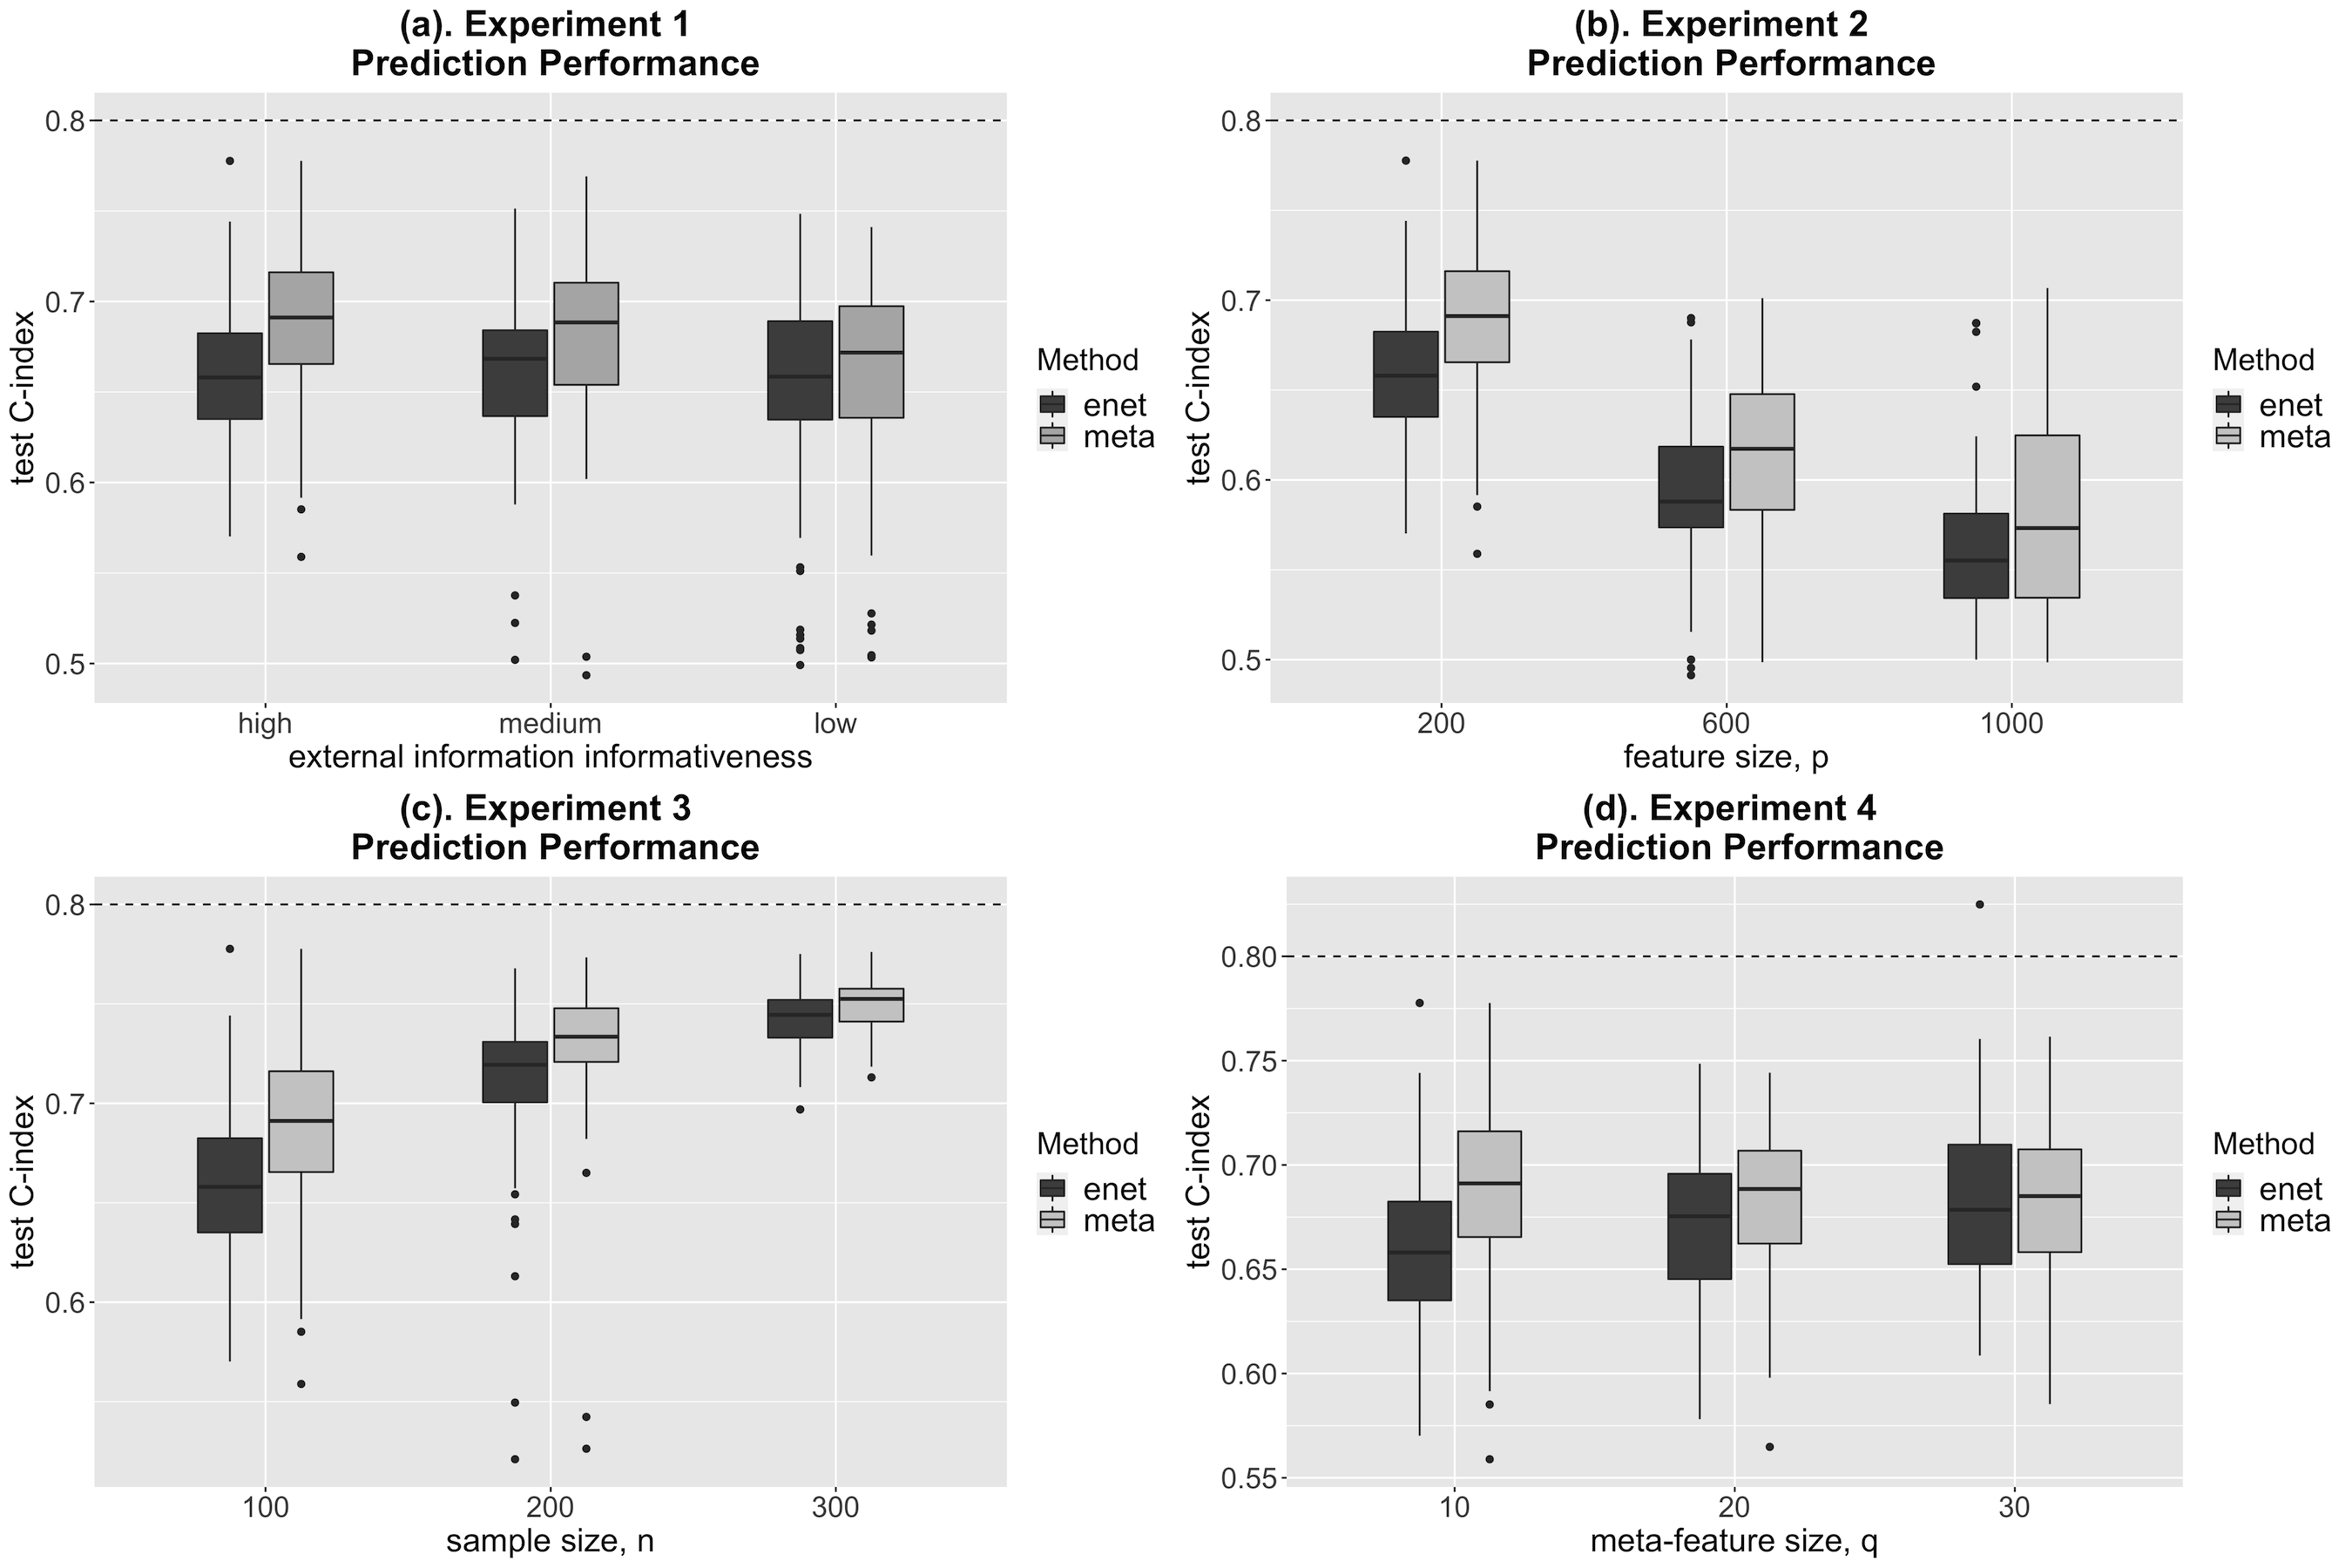
\includegraphics[width=\textwidth]{sim21}
    \caption{Simulation: prediction performance }
    \label{fig:sim21}
\end{figure} 

\begin{figure}
    \centering
    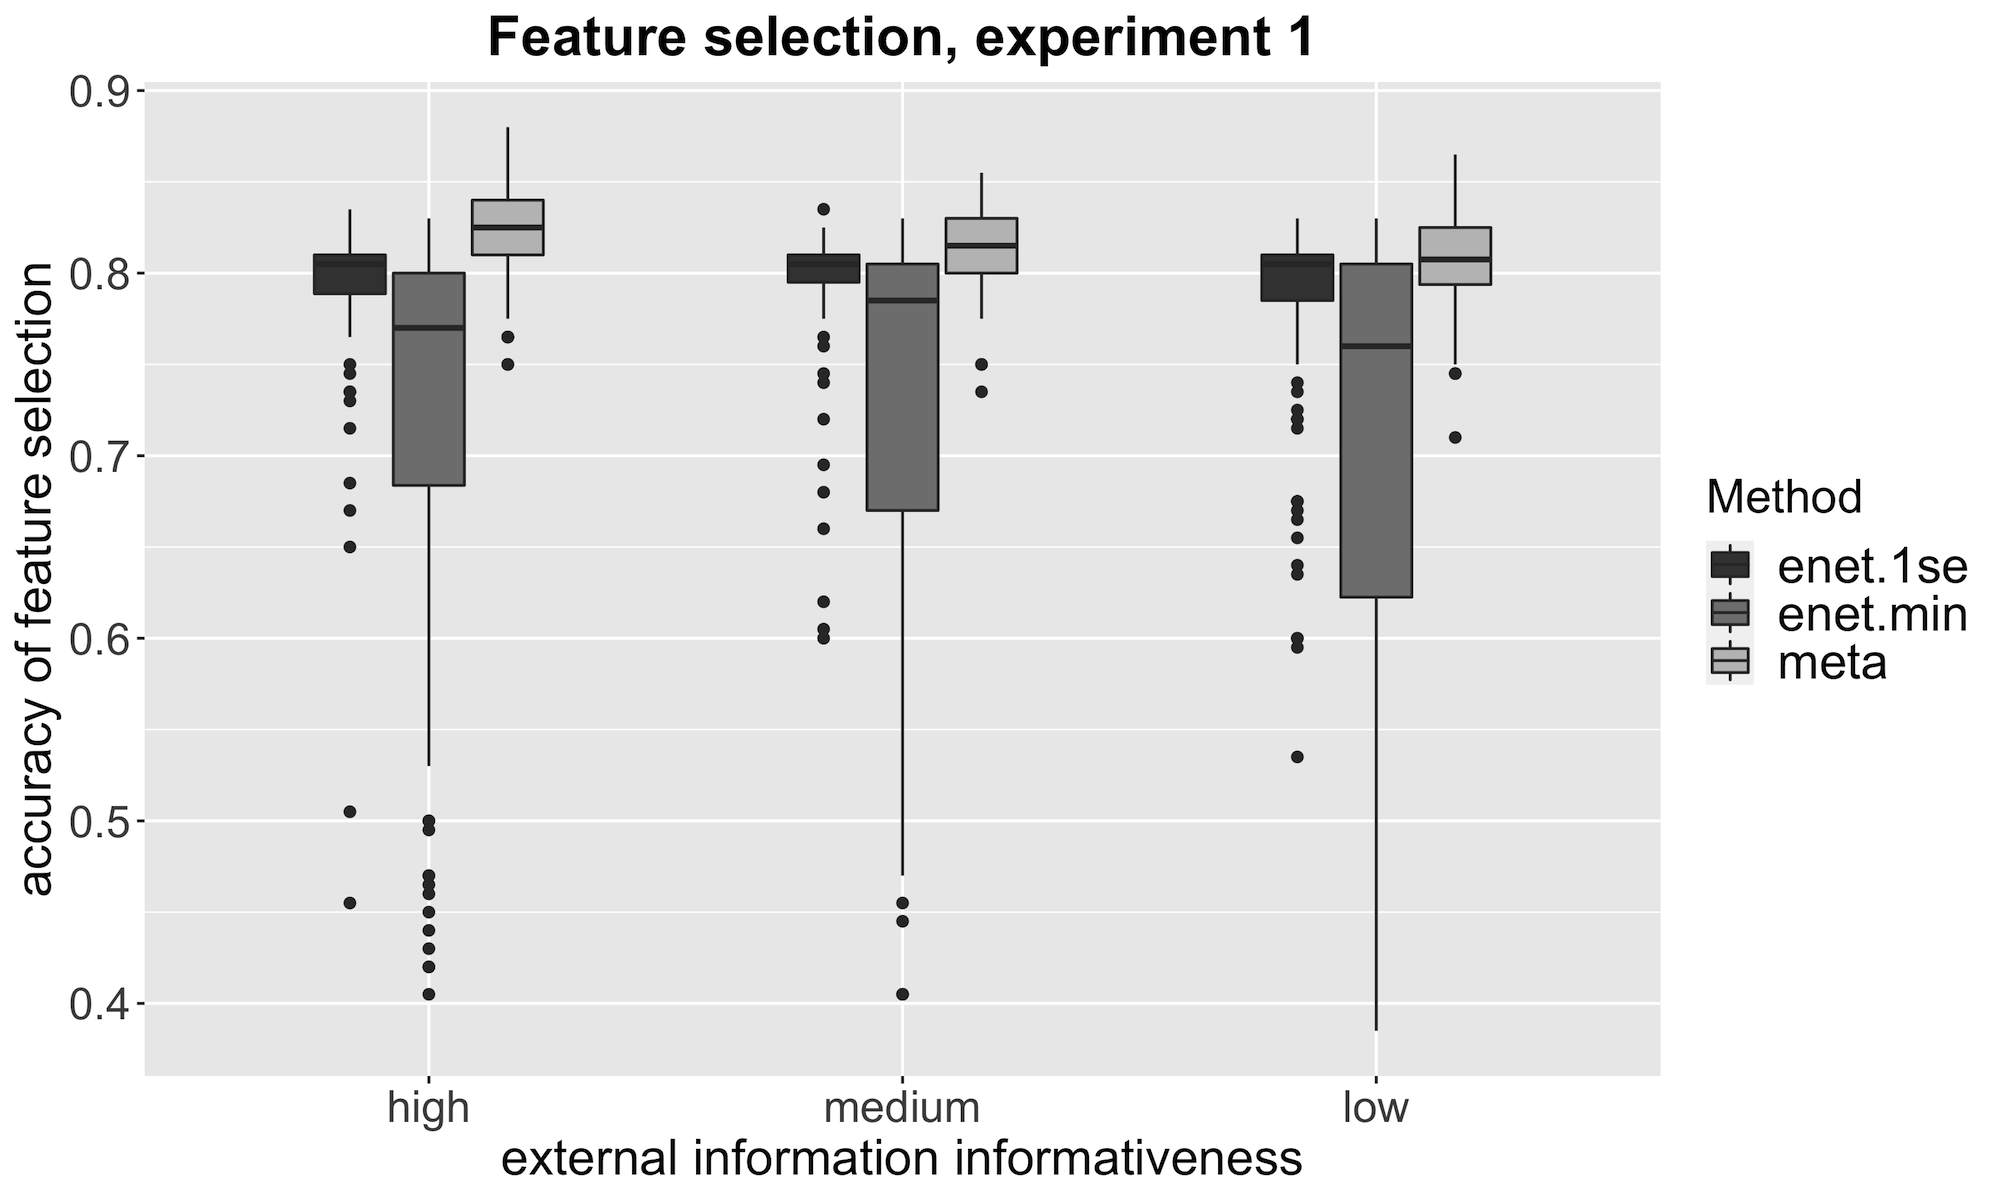
\includegraphics[scale=0.7]{sim22}
    \caption[Simulation: feature selection]{Simulation: feature selection. `enet.min' is the standard elastic net model with the $\lambda$ value that gives maximum cross-validated C-index; `enet.1se' is the elastic net model with the $\lambda$ value that gives the most regularized model such that the cross-validated C-index is within one standard error of the maximum.}
    \label{fig:sim22}
\end{figure}

\section{Applications}
We also applied the proposed meta-feature model to a melanoma data set to predict overall survival in patients treated with PD-1 immune checkpoint blockade. The programmed death 1 pathway (PD-1) is an immune-regulatory mechanism used by cancer to hide from the immune system. Antagonistic antibodies to PD-1 pathway and its ligands, programmed death ligand 1 (PD-L1), demonstrate high clinical benefit rates and tolerability. Immune checkpoint blockades such as Nivolumab, pembrolizumab are anti-PD-1 antibodies showing improved overall survival for the treatment of advanced melanoma. However, less than 40\% of the patients respond to the treatments \citep{moreno2015anti}. Therefore, predicting treatment outcomes, identifying predictive signals are of great interest to appropriately select patients most likely to benefit from anti-PD-1 treatments. We explored transcriptomes and clinical data using our model to illustrate prediction performance and predictive signal selection.

The dataset combined 3 clinical studies in which RNA-sequencing were applied to patients treated with anti-PD1 antibodies, \cite{gide2019distinct, riaz2017tumor, hugo2016genomic}. The gene expression values are normalized toward all sample average in each study as the control, so that they are comparable to one another across features within a sample and comparable to one another across samples. There are 16010 gene in common across 3 studies, and combined 117 subjects. The clinical variables being considered are age, gender, and tumor response. We build predictive models in terms of overall survival, based on transcriptomics and clinical variables. Since the subjects are all treated with anti-PD1 antibodies, the transcriptomic features selected by the model are predictive signals for treatment efficacy or resistance. We selected meta-features from molecular signature database, hallmark gene sets \citep{liberzon2015molecular}. 13 gene sets are enriched \citep{subramanian2005gene} to have false positive rates less than 0.25 (Table \ref{table3.1}). An indicator matrix is formed to illustrate whether each of the 16010 genes belong to one of the 13 hallmark gene sets ($\bm{Z}$). 

We compared prediction and feature selection performance between meta-feature guided elastic net model and standard elastic net model. The data is split into training and test set (3:1). Standard elastic net is trained using 5-fold cross validation, while meta-feature model is trained with estimated hyperparameters. The test concordance index is 0.7340 for the elastic net, and 0.7609 for our meta-feature guided model. As for feature selection, the meta-feature model, which selects 4 transcriptomes (GPAA1, COX6C, VPS28, PLCB4), is sparser, as opposed to 11 features selected in the elastic net model. 
\begin{table}[tbh]
    \centering
    \def\arraystretch{1.3}
    \begin{tabular}{|c|c|}
    \hline
     \bf Hallmark meta-feature & \bf Estimated $\bm{\alpha}$ \\
     \specialrule{.1em}{.05em}{.05em}
     Interferon gamma response & -0.0102  \\ \hline
     Allograft rejection & 0.1570  \\ \hline
     Interferon alpha response & -0.0314 \\ \hline
     IL6 JAK STAT3 signaling & 0.1131 \\ \hline
     Inflammatory response & 0.0744 \\ \hline
     Complement & 0.1577 \\ \hline
     TNFA signaling via NFKB & 0.1180 \\ \hline
     IL2 STAT5 signaling & 0.1613 \\ \hline
     Bile acid metabolism & 0.0876 \\ \hline
     Kras signaling down & 0.2338 \\ \hline
     Xenobiotic metabolism & 0.2598 \\ \hline
     Apoptosis & 0.2557 \\ \hline
     Kras signaling up & 0.2737 \\ \hline
    \end{tabular}
    \caption[List of hallmark meta-features and their respective estimated weight]{List of hallmark meta-features and their respective estimated weight $\bm{\alpha}$. Weights are estimated from empirical Bayes hyperparameter tuning.}
    \label{table3.1}
\end{table}

\section{Discussion}
In this paper, we extended to survival outcome a customized regularization model guided by genomic meta-features. This model has unique penalty parameters for each of the features instead of one common penalty parameter for all the features in standard regularized regression. This differential penalty amount allows each feature to be of different importance to the outcome of interest, guided by their underlying characteristics. With the feature characteristics highly informative, the important features will be penalized less (less shrinkage, less likely to be 0), and the not so important features will be penalized heavier (heavier shrinkage, more likely to be 0, excluded from the model), so that achieving better feature selection. For the range of simulation results and data application in anti-PD1 immunotherapy predictive modeling, the customized regularization model showed benefits in prediction performance, and the selected model tend to be sparser (less features selected). Note that we do need the external meta-feature data to be informative with less noise meta-features, because the proposed model does not predicts as well with the increase in dimension of meta-features. Therefore, we need prior knowledge to select meta-features. However, the proposed model is a systematic way to incorporate external meta-features that will most likely provide insight on how to further modeling the data.

In the setting of incorporating meta-feature into regularized regression, we have developed 2 methods to systematically utilize them in modeling process. The method in this paper integrates meta-features in a non-linear way. It allows the meta-features to decide the importance of each feature by defining the penalty parameters as a non-linear function of meta-features. As opposed to this method, Weaver et al. [] and Shen et al. [] integrates meta-features linearly, which implemented in R package `xrnet'. The fundamental difference between the 2 methods is that `xrnet' models meta-features through the mean of $\bm{\beta}$, while the proposed model in this paper models meta-features through the variance of $\bm{\beta}$. As they both have underlying hierarchical structure to model features and meta-features, `xrnet' assumes meta-features are a linear regression of feature regression coefficients, $\bm{\beta} \sim N(\bm{Z\alpha}, \tau\bm{I})$, therefore, the mean of $\bm{\beta}$ is determined by $\bm{Z\alpha}$. In the customized regularization model, $\bm{\beta}$ has an approximated prior $N(0, \frac{2}{2\lambda_j(1-c)+c^2\lambda_j^2})$, we can see the variance is determined by meta-features. In practice, it is hard to tell which one is in favor to another. Depending on the application at hand, one would want to try both as different data has different dynamics. 

Our proposed model applied empirical Bayes to estimate penalty parameters for each feature, which uses Laplace approximation to obtain the marginal likelihood. Laplace approximation works well when sample size is relatively large. We see in simulation experiment 2, while our model shows prediction benefits in all feature sizes, there is a decreasing trend of benefits over standard elastic net Cox regression, which might caused by the drop of quality in Laplace approximation when sample size is too small relative to feature size. We did not fully address how well Laplace approximation is in the modeling process, and how it will affect the model performance. We need to be careful when applying the model to ultra high dimensional data. 

We have mentioned that the proposed customized regularization model does not handle higher dimension of meta-features very well. This is because no regularization is applied to meta-feature weights $\bm{\alpha}$, or control its complexity in some form. As a result, the model fitting algorithm is not able to deal with large number of meta-features efficiently and stably. Careful selection of meta-features is needed rather than fitting all external information at hand. In simulation experiment 4, the prediction improvement decrease as we increase the number of meta-features. With continuous development of gene annotation database, more summary statistics from meta-analyses, future work in regularizing meta-features is a potential improvement of the model to expand its ability of handling high dimensional meta-feature data.


% Research Topic 3
\chapter{\texorpdfstring{$L_0-$}{Lg}Regularized Regression with Correlated Features}
\label{cha:L0}

\section{Introduction}
In chapter \ref{cha:introduction},  we discussed the feature selection properties of the lasso, elastic net, and best subset selection. The latter is equivalent to $L_0$ constrained regression when data matrix $\bm{X}$ is orthogonal. In fact, the lassso and elastic net can be thought of as approximation methods to best subset selection. We see this in section \ref{sec:nonconvex}; in the spectrum of $L_q$ constrained regression, $q=0$ corresponds to best subset selection, $0<q<1$ to nonconvex regularization, $q=1$ to the lasso, and $q=2$ to ridge regression, which does not perfom selection. As the value of $q$ moving away from 0 to larger values, the estimated regression coefficients become more biased toward 0, and the resulting model becomes less sparse. Under orthogonality of the design matrix, best subset selection ($L_0$) yields unbiased coefficient estimates. Therefore, $L_0$ constrained regression would be generally the preferred model. However, in reality the features are not orthogonal, and exhibit some degree of correlations. In this situation, the $L_0$ constrained regression is an NP-hard problem \citep{huo2007stepwise}. 

Several approaches have been proposed for fitting the $L_0$-regularized linear regression. \cite{blumensath2008iterative} introduced an iterative hard thresholding algorithm, which is a proximal gradient-based method. Based on hard thresholding, several variants of the method have also been developed, such as proximal iterative hard thresholding \citep{zhang2019new}, and proximal alternating iterative hard thresholding \citep{yang2017proximal}. These methods share the main idea of applying the proximal operator univariately to obtain coordinate-wise solutions. However, these methods ignore the correlation structure of the data matrix $\bm{X}$, and might not work well with correlated features. We look at a novel algorithm to $L_0$ constrained least squares  and modify it to incorporate the covariance matrix $\bm{X}^T\bm{X}$ into account. The original plan for this work was to later extend $L_0$ constrained least squares to integrate meta-features. However, the approach did not work as expected and we turned to the methods in Chapters 2 and 3 instead. We include it here for completion and because some of the ideas may prove useful in the future.

\section[Proximal distance algorithm for \texorpdfstring{$L_0-$}{Lg}regularized regression]{Proximal distance algorithm for \texorpdfstring{$L_0-$}{Lg}regularized regression}
Proposed by \cite{keys2019proximal}, the proximal distance algorithm is a general method for solving a constrained optimization problem. It converts a constrained minimization problem into an unconstrained one, with a penalty on the distance to the constrain set. The constrained minimization problem is 
\begin{equation} \label{prox_con}
\begin{aligned}
    & \min_{x\in \mathbb{R}^p} f(x), \\
    & \text{subject to} \hspace{0.6cm} x\in C, 
\end{aligned}
\end{equation}
where $C$ is a closed set. This general constrained optimization problem can be turned into a penalized version (unconstrained)
\begin{equation} \label{prox_uncon}
   \min_{x\in \mathbb{R}^p} f(x)+\frac{\rho}{2}\text{dist}(x,C)^2,
\end{equation}
where the squared distance is defined as $\text{dist}(x,C)^2=\inf_{y\in C}\|x-y\|_2^2$, i.e. the square of the Euclidean distance of $x$ to the closed set $C$. The distance penalty function is nonnegative and vanishes precisely on $C$. As the penalty parameter $\rho$ tends to $\infty$, the distance of $x$ to set $C$ is penalized so strongly that it is close to 0, i.e., $x$ is in the set, which means the minimizer found by the unconstrained version \eqref{prox_uncon} is equivalent to the constrained one \eqref{prox_con}. To minimize \eqref{prox_uncon}, we again use a majorization-minimization (MM) algorithm similar to that used in chapter \ref{cha:xtunecox} to estimate the model hyperparameters. The majorization step, which forms an upper bound of $f(x)$ around the current iterate $x_n$, replaces the distance penalty function $\text{dist}(x,C)^2$ with the spherical quadratic $\|x-P_C(x_n)\|_2^2$, where $P_C(x_n)$ is the projection of the $n^{th}$ iterate $x_n$ onto C: the point in set C that attains the minimum distance to the point, $P_C(x_n)=\argmin_{x\in C}\|x_n-x\|_2$. Therefore, by the definition of projection, $\|x-P_C(x_n)\|_2^2\geq\text{dist}(x,C)^2$, and at current iterate $x_n$, the tangency condition, $\|x_n-P_C(x_n)\|_2^2=\text{dist}(x_n,C)^2$ of a majorization is satisfied. The minimization step is then the proximal map of the current projection
\begin{equation}
    x_{n+1}=\text{prox}_{\rho^{-1}f}(P_C(x_n))=\argmin_x f(x)+\frac{\rho}{2}\|x-P_C(x_n)\|_2^2.
\end{equation}
The MM principle guarantees that $x_{n+1}$ decreases the penalized loss.

For the $L_0$-regularized least squares problem, the constrained optimization form can be written as 
\begin{equation} \label{L0_con}
    \begin{aligned}
    \min_{\beta\in \mathbb{R}^p} \frac{1}{2}\|y-\bm{X}\beta\|_2^2, \\
    \text{subject to} \hspace{0.6cm} \beta \in S_k^p,
    \end{aligned}
\end{equation}
where $S_k^p$ is the set of vectors with at most $k$ nonzero entries out of $p$. The unconstrained form of \eqref{L0_con}, i.e., the penalized distance objective function is
\begin{equation} \label{L0_uncon}
    \min_{\beta\in \mathbb{R}^p} \frac{1}{2}\|y-\bm{X}\beta\|_2^2+\frac{\rho}{2}\text{dist}(\beta, S_k^p)^2.
\end{equation}
To use the majorization-minimization algorithm to solve problem \eqref{L0_uncon}, first we perform distance majorization
\begin{equation}
    \min_{\beta\in \mathbb{R}^p} \frac{1}{2}\|y-\bm{X}\beta\|_2^2+\frac{\rho}{2}\|\beta-P_{S_k^p}(\beta_n)\|_2^2.
\end{equation}
The minimization step is the proximal operator of the projection onto set $S_k^p$,
\begin{equation}
    \beta_{n+1}=\text{prox}_{\rho^{-1}\text{OLS}}(P_{S_k^p}(\beta_n))=(\bm{X}^T\bm{X}+\rho\bm{I})^{-1}(\bm{X}^Ty+\rho P_{S_k^p}(\beta_n)).
\end{equation}
We discussed earlier that the distance penaly parameter $\rho$ should be increased systematically until a constrained minimum is reached. In practice, starting $\rho_0=1$, and increasing its value through a sequence $\rho_n=\min(\alpha^n\rho_0, \rho_{\max})$ with  $\alpha$ slightly larger than 1 works well. The overall algorithm can be summarized as follow:
\begin{enumerate}
    \item Initialize $\beta_0=1$, $\rho_0=1$, $\text{dist}_0=\infty$, $\text{loss}_0=\infty$,
    \item For iteration counter $n$ from $1$ to max iteration:
    \begin{enumerate}
        \item Update $\beta_n=\text{prox}_{\rho^{-1}OLS}(P_{S_k^p}(\beta_{n-1}))$
        \item Current distance $\text{dist}_n=\|\beta_n-P_{S_k^p}(\beta_{n-1})\|_w^2$
        \item Current loss function vaue $\text{loss}_n=OLS(\beta_n)$
        \item If $|\text{dist}_n-\text{dixt}_{n-1}|<\text{tolerance}$ and $|\text{loss}_n-\text{loss}_{n-1}|<\text{tolerance}$:
        \begin{itemize}
            \item break
            \item return $P_{S_k^p}(\beta_n)$
        \end{itemize}
        else:
        \begin{itemize}
            \item $\text{dist}_{n-1}=\text{dist}_n$
            \item $\text{loss}_{n-1}=\text{loss}_n$
            \item increase $\rho$ by a small multiplier $\alpha$ every few iterations
        \end{itemize}
    \end{enumerate}
\end{enumerate}

\section{Incorporating the data covariance matrix}
The proximal distance algorithm uses the Euclidean distance as the distance metric. But this ignores the correlations between features. To incorporate the covariance matrix, we can use the weighted distance (Mahalanobis distance):
\[
d(x,y)=\sqrt{(x-y)^T\bm{W}^{-1}(x-y)},
\]
where, assuming the columns of $\bm{X}$ are mean-centered, $\bm{W}=\bm{X}^t\bm{X}$ is the data covariance matrix. With weighted distance majorization, the new update is 
\begin{equation}
    \beta_{n+1}=\text{prox}_{\rho^{-1}\text{OLS}}(P_{S_k^p}(\beta_n))=(\bm{X}^T\bm{X}+\rho\bm{W})^{-1}(\bm{X}^Ty+\rho\bm{W} P_{S_k^p}(\beta_n)).
\end{equation}
However, we need to project the current iterate to the $L_0$ constraint set, $P_{S_k^p}(\beta_n)$. With the standard Euclidean distance, the projection simply keeps the largest $k$ coordinates of $\beta$ and the remaining coordinates are set to 0. With the weighted distance, the projection problem is again NP-hard. We notice that if the weight matrix is diagonal, the projection keeps the $k$ coordinates with largest value of $w_j\beta_j^2$. Based on this observation, we propose the following approximation to the projection: for each coordinate $j$, compute the value $\frac{e_j^T\bm{W}\beta}{e_j^T\bm{W}e_j}$, which is the weighted projection onto axis $j$, and keep the axis projection value $\frac{(e_j^T\bm{W}\beta)^2}{e_j^T\bm{W}e_j}$, while setting the  rest of the coordinates to 0. This is similar to the projection method with the standard Euclidean distance but in a weighted inner-product space. 

\section{Simulation}
We simulated a data matrix $\bm{X}$ of dimension $100\times 200$, following a multivariate normal distribution, $N(0, \Sigma)$, where $\Sigma$ has an autoregressive(1) correlation structure with $\rho=0.1$, i.e., features are close to uncorrelated.  Regression coefficients $\bm{\beta}$ are also simulated with $N(0, \Sigma_\beta)$, where $\Sigma_\beta$ is autoregressive(1) with $\rho=0.6$. The variance components of $\bm{\beta}$ (diagonal elements of $\Sigma_\beta$) are set to be large for the first 10 elements, and small for the remaining 190. This setting makes the true underlying model sparse, i.e., the first 10 elements of $\bm{\beta}$ are non-zero, and the rest are all zeros. The data true predictive $R^2$ is fixed at $R^2=0.5$. Hyper-parameters of of the lasso ($\lambda$) and $L_0$ ($k$) are tuned using a simulated validation set. The experiment is repeated 100 times. The results (Table \ref{table:4.1}) showed that the validation $R^2$ of the lasso is higher than the validation $R^2$ for standard $L_0$ regression. In terms of feature selection, the true positive selection rate of lasso is also better than that of $L_0$ regression. However, this comes at the price of a higher false positive rate. We also looked at the bias of the first element of $\bm{\beta}$, where bias is the absolute value of the difference between the true value and the estimated value. The average bias of signal 1 of $L_0$ regression is much smaller than for the lasso.
\begin{table}[tbh]
    \centering
    \def\arraystretch{1.5}
    \begin{tabular}{|c|c|c|c|c|}
        \hline
         & \textbf{Validation $R^2$} & \textbf{Ture positive rate} & \textbf{False positive rate} & \textbf{Bias} (signal 1)  \\ 
        \specialrule{.1em}{.05em}{.05em}
        $L_0$ & 0.268 & 0.506 & 0.019 & 0.231 \\ 
        \hline
        lasso & 0.318 & 0.770 & 0.114 & 0.394 \\ 
        \hline
    \end{tabular}
    \caption{Prediction and feature selection comparison between lasso and $L_0$}
    \label{table:4.1}
\end{table}

We then looked at the 10 true signal coefficient estimates from a single run of the above experiment. Estimates from standard $L_0$ regression, our proposed weighted $L_0$ regression incorporating the data correlation structure, the lasso, along with the simulated true values are compared (Figure \ref{fig:L_0}). The standard $L_0$ selected 5 out of 10 true signals, while weighted $L_0$ and lasso both chose 8 of them. However, lasso estimates are heavily shrunk. Note that we used weighted distance metric in the weighted $L_0$ algorithm, but with the standard projection. 
\begin{figure}[tbh]
  \centering
  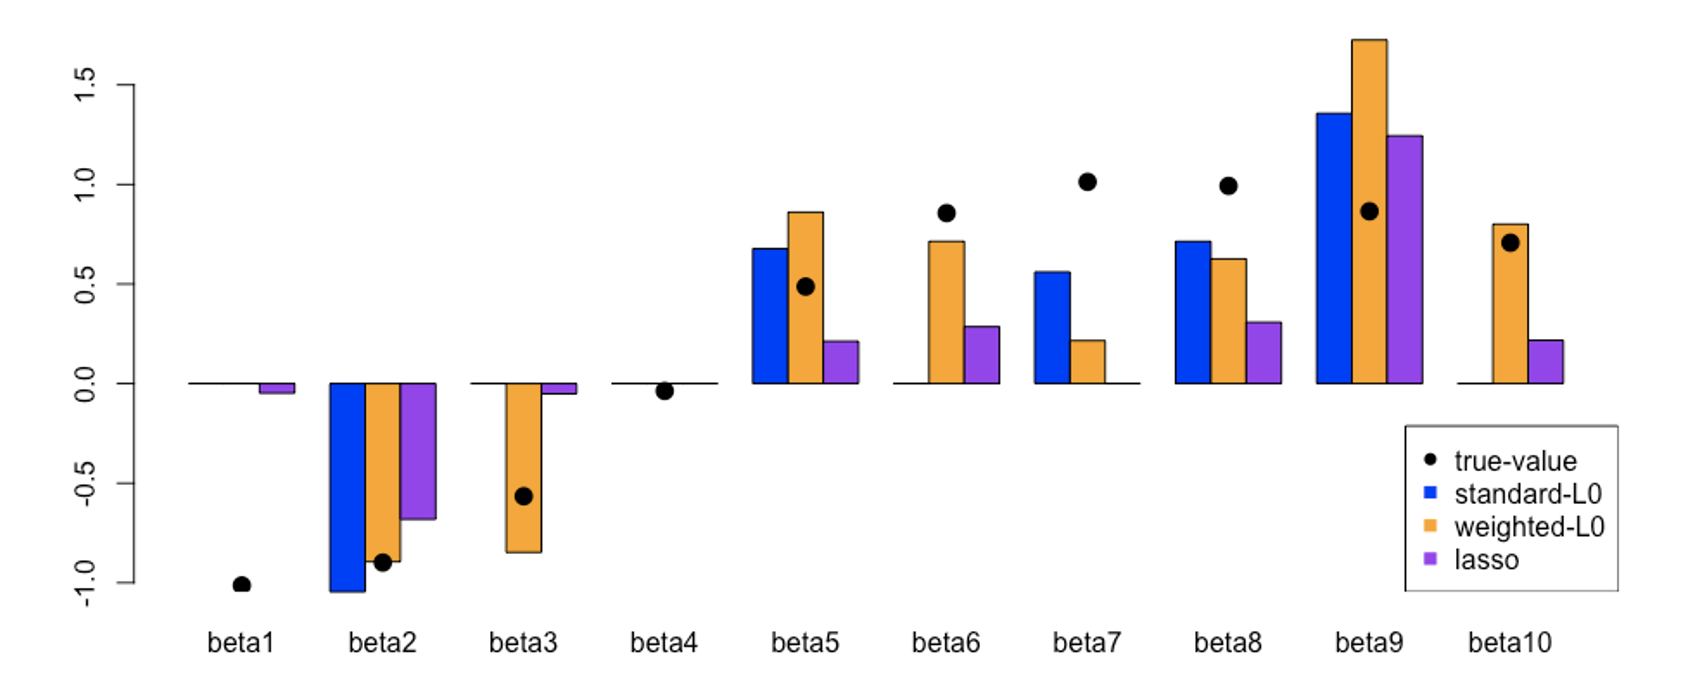
\includegraphics[width=\textwidth]{L_0}
  \caption{Comparison of signal estimates}
  \label{fig:L_0}
\end{figure}

The simulation results showed some potential for the weighted $L_0$ algorithm to improve feature selection in terms of accuracy and bias of the estimates. However, when we tried the proposed approximate solution to weighted projection in simulation, the results didn't show improvement in feature selection, and we haven't come up with a better solution to the weighted projection problem. 


% Conclusion and ongoing work
\chapter{Discussion and future work}
\label{cha:conclusion}

\section{Discussion on genomics data integration}
The purpose of this thesis is to develop novel modeling methods predicting health outcomes, based on genomics data. As the types and the volume of genomics data are huge thanks to advanced high-throughput sequencing technologies, as well as the ever-growing annotation databases, there is increased need to integrate multiple types of genomics data, annotation data into modeling process. Because related variables provide more information to the health outcomes of interest, and hence improve prediction performance. The traditional method is modeling one type of genomics data at a time, and combine the models in some form. As to utilizing annotation data, summary statistics, it is usually performed after modeling genomics data. This style of modeling different genomics data separately may ignore the interplay between them, the collective effect on the outcome. In this thesis, we introduced the concept meta-features, the features of the features, to incorporate external data. And we also introduced a meta-feature data matrix $\bm{Z}$ that systematically stores the external data. In the two methods developed in the thesis, chapter \ref{cha:xrnetcox}, \ref{cha:xtunecox}, we mainly discussed how to put annotation information into meta-feature matrix. That is, if we have $p$ genomic features, $q$ functional gene sets (meta-features), the meta-feature matrix $\bm{Z}$ will have dimension $p\times q$, each row represents one genomic feature and has values of 0 or 1 indicating whether this genomic feature belongs to a gene set (1 indicates it belongs to the gene set, and 0 not). However, the usage of meta-feature matrix does not limit to annotation data, in fact, it can accommodate many types of information. We discuss 2 situations to show the flexibility of putting external data into meta-feature matrix $\bm{Z}$.

\begin{itemize}
    \item There are 3 types genomics data, gene expressions, single nucleotide polymorphisms (SNPs), DNA methylation  to be integrated into the modeling process. The meta-feature matrix tells which genomic feature is SNP, gene expression, or methylation. Table \ref{table:d1} shows the indicator meta-feature matrix. For example, ILMN\_343291 is a microarray probe, gene expression; rs10853372 is a SNP locus. 
    \begin{table}[tbh]
    \centering
    \def\arraystretch{1.5}
    \begin{tabular}{|c|c|c|c|}
        \hline
         & \textbf{Gene expression} & \textbf{SNP} & \textbf{Methylation} \\ 
        \specialrule{.1em}{.05em}{.05em}
        ILMN\_343291 & 1 & 0 & 0 \\ 
        \hline
        rs10853372 & 0 & 1 & 0 \\ 
        \hline
        ILMN\_1651210 & 1 & 0 & 0 \\
        \hline
        463100A3 & 0 & 0 & 1 \\
        \hline
        \vdots & \vdots & \vdots & \vdots \\
    \end{tabular}
    \caption{Meta-feature matrix $\bm{Z}$ for multiple types of genomics data}
    \label{table:d1}
    \end{table}
    
    \item There are summary statistics from similar studies on the same set of genomic features. These statistics from meta-analysis can be highly informative. They include p-values, hazard ratios, and source of features. In table \ref{table:d2}, gene BAX has a p\_value 0.0006 associated with the outcome, hazard ratio is 0.7605, the reason being included in the model is from previous GWAS studies. This is a hybrid matrix holding continuous values and indicator values: continuous values like p\-values, hazard ratios gives importance of the features; indicator variable tells the reason why the feature is included. 
    \begin{table}[tbh]
    \centering
    \def\arraystretch{1.5}
    \begin{tabular}{|c|c|c|c|c|c}
        \hline
         & \textbf{p\_value} & \textbf{Hazard ratio} & \textbf{Literature} & \textbf{GWAS}  \\ 
        \specialrule{.1em}{.05em}{.05em}
        BAX & 0.0006 & 0.7605 & 0 & 1 & \dots \\ 
        \hline
        IL6 & 0.2611 & -0.2077 & 1 & 0 & \dots \\ 
        \hline
        LDHB & $8.78\times 10^{-6}$ & 0.0768 & 0 & 1 & \dots \\
        \hline
        \vdots & \vdots & \vdots & \vdots & \vdots & $\ddots$ \\
    \end{tabular}
    \caption{Meta-feature matrix $\bm{Z}$ for summary statistics}
    \label{table:d2}
    \end{table}
\end{itemize}

With the above examples, we are shown the flexibility of the meta-feature matrix housing external information. Through the meta-feature matrix, we can integrate multiple types of genomics data, genomic annotation data, summary statistics from similar studies, and so on. It is the heart of our modeling process to integrate extra information that might be useful to prediction.

\section{Discussion on high dimensionality of genomics data}
Most of the genomics data are high dimensional. The human genome contains approximately 3 billion base pairs, which reside in the 23 pairs of chromosomes within the nucleus of all our cells. Each chromosome contains hundreds to thousands of genes, which makes around 30,000 genes in the human genome. SNPs are common genetic variants happens roughly 1\% of the times among 3 billion base pairs in the human genome, so there are about 10 million SNPs. Over the years, many SNPs have been found. The number of genomics features, e.g., gene expressions, SNPs, DNA methylation, is huge by nature. However, the number of samples, especially in oncology setting, is small relative to the amount of genomics. For cancer patients, genomics data are obtained by tissue biopsy, which can be highly invasive, risky, costly. Some tumor locations are hard to access. And cancer patients are usually under serious health conditions which also prevent them from tissue biopsy. As a result, the number of patients with genomics data is limited. A typical data set in cancer genomics consists of hundreds to thousands subjects, and the number of genomic variables is tens to hundreds thousands, even millions. This makes the data ultra high dimensional ($p>>n$). We have already discussed in high dimensional setting, regularized regression as a linear model, is one of the better options, since every variable contributes a little to none effect to the outcome of interest. Intuitively, considering coming up a surface to classify samples in a high dimensional space, it is easy to use a hyperplane than a complicated non-linear surface. It is the opposite in a relatively low dimensional space, where non-linear pattern is favored. 

Recently, a novel technique, liquid biopsy which takes the human blood sample instead of tumor tissue, has been explored. It is less invasive, painful, easy to access, and can be performed in most health conditions. This could potentially generate more samples than tissue biopsies, and high dimensionality may no longer be an issue for genomics data. With both samples and features in high dimension, simple models such as linear models are not among the best any more. As machine learning has made great progress over the past years, there are better modeling choices. Reconsidering the claim that each genomic feature contribute a little to none effect to the outcome. While this is true, there could also be non-linear patterns like interactions between features that for example, over expression of one gene could cause other genes' expression change. Under limited samples, these complicated patterns are impossible to detect due to lack of information. However, with more samples, it is possible, and there are better models for exploring non-linear patterns. Gradient boosting machine is a tree-based method that specializing in detecting complicated interaction patterns. Deep neural network, with enough units and layers, can mimic any non-linear patterns. These two methods are hugely successful recently, because almost every data has some form of non-linear pattern. And we do see they need large amount of instances/samples to be successful. Liquid biopsy provides us the possibility to have large sample size while the number of genomic features remains large. Although it is not fully validated yet, in the near future, it can be expected to make impact on cancer genomics. As in cancer genomics, complicated non-linear pattern like square, higher order polynomials are hard to interpret the effects of genomics. Gene-gene interactions, gene-environment interactions, or even higher order interactions are of great interest. Therefore, in the case of having plenty of samples, developing methods to integrate genomics data for gradient boosting machine is a meaningful future work.

\section {Discussion on feature selection}
Up to now, the feature selection that we talked about is selecting a subset of the features that already included in the modeling process. Precisely speaking, this process is subset selection, which is to produce a parsimonious model that can reveal the underlying association between features and outcomes. Before further discussing subset selection, we first talk about feature selection, the process of selecting related features to build a predictive model. The predictive modeling process starts with laying out the question: what is the purpose of the predictive model, what type of outcome is to be predicted. Based on the scientific questions, we choose the data to collect that will give the most predictive power. In cancer genomics, data from tissue biopsy may contain different types of genomics data. It is not much of a problem to decide the types of data to be used based on the purpose, but rather, within one type of data, what subset of features to be included in the model. Because of the high dimensionality of data, one might want to narrow down the set of genomic features that have more predictive power. One common approach that is not recommended is to let the data decide the set of features by conducting pre-analysis based on the data. Because pre-screening the features based on the data and building predictive model afterwards is equivalent to using the data twice for modeling. It is problematic to train the model twice on different training sets. What can be done is utilizing knowledge from past studies, literature. But still, it is not a good idea to pre-screening features at all. The features that are considered not important may multivariately work with other features to be predictive to the outcome. Regularized regression has the ability to exclude unimportant features by shrink them to 0; gradient boosted trees can ignore those features by not even using them as tree nodes. It is better to let the model decide how each feature contributes to prediction.

Now in terms of subset selection in regularized regression, the two methods developed in this thesis both used most common sparse regularization technique, the lasso and the elastic net. Because they are both convex, and have stable and efficient algorithms. Moreover, as we discussed in section \ref{sec:sparse}, the lasso subset selection is consistent under certain conditions, and the elastic net can complement the lasso to deal with group correlated features. However, as convex approximations to best subset selection, they both produce estimators biased toward 0, and there exist some conditions in which their subset selection are not consistent. Discussed in section \ref{sec:nonconvex}, nonconvex regularizations, which are more closer approximations to best subset selection, produce more parsimonious model, and the estimators are less biased toward 0. The 2 nonconvex regularizations that are discussed, the SCAD and the MCP, along with the adaptive lasso, approximation to $L_q (0<q<1)$ regularization, enjoy oracle property; namely, when the true estimators have some zero components, they are estimated as 0 with probability tending to 1, and the nonzero components are estimated as well when the correct submodel is known \citep{fan2001variable}. This property improves the model accuracy compared to the lasso and the elastic net. As the 3 regularization techniques enjoy coordinate descent algorithm, they are natual extensions to the two methods developed in this thesis, for the purpose of better subset selection, in terms of both accuracy and unbiased estimator. 

\section{Discussion on statistical inference}

% Using single-space for reference list.
\begin{singlespace}
% Bibliography
\phantomsection
\addcontentsline{toc}{chapter}{References}%
\markboth{References}{References}%
% If you use BibLaTeX
%\printbibliography[title=References]
% If you use BibTeX
% \bibliographystyle{plain}
\bibliography{references}
\end{singlespace}

% Appendices
\phantomsection
\addcontentsline{toc}{chapter}{Appendices}%
\markboth{Appendices}{Appendices}%
\chapter*{Appendices}
\renewcommand\thesection{\Alph{section}}
\renewcommand*{\thesubsection}{\Alph{section}.\arabic{subsection}}
\begingroup
\numberwithin{equation}{section}
% Appendix source files
\section{Appendix for chapter 2}

\subsection{Computation of diagonal elements of weight matrix}
\label{a.1}
Diagonal elements of weight matrix $\bm{W}$, the Hessian of log of Cox'x partial likelihood function, has the form 
\begin{displaymath}
w_i=\sum_{k\in C_i}\frac{d_k e^{\tilde{\eta}_i}}{\sum_{j\in R_i}e^{\tilde{\eta}_j}}-\sum_{k\in C_i}\frac{d_k (e^{\tilde{\eta}_i})^2}{(\sum_{j\in R_i}e^{\tilde{\eta}_j})^2}. 
\end{displaymath}
The two sums $\sum_{k\in C_i}$ and $\sum_{j\in R_i}$ both have $n$ elements, hence it is a $O(n^2)$ computation. However, if we notice the difference between $R_k$ and $R_{k+1}$ is the observations that are in $R_k$ but not in $R_{k+1}$, i.e., $\{j:t_k\leq y_j < t_{k+1}\}$, provided that the observed times $\bm{y}$ are sorted in non-decreasing order, then $\sum_{j\in R_k}e^{\tilde{\eta}_j}$ can be calculated as cumulative sums:
\begin{displaymath}
\sum_{j\in R_k} e^{\tilde{\eta}_j} =\sum_{j\in R_{k+1}} e^{\tilde{\eta}_j}+ \sum_{j\in R_k \& j\notin R_{k+1}} e^{\tilde{\eta}_j}.
\end{displaymath}
The same cumulative sum idea can be applied to $\sum_{k\in C_i}$: 
\begin{align*}
    \sum_{k\in C_{i+1}}\frac{d_k e^{\tilde{\eta}_i}}{\sum_{j\in R_i}e^{\tilde{\eta}_j}}&=\sum_{k\in C_i}\frac{d_k e^{\tilde{\eta}_i}}{\sum_{j\in R_i}e^{\tilde{\eta}_j}}+\sum_{k\in C_i\&k\notin c_{i+1}}\frac{d_k e^{\tilde{\eta}_i}}{\sum_{j\in R_i}e^{\tilde{\eta}_j}}, \\
    \sum_{k\in C_{i+1}}\frac{d_k (e^{\tilde{\eta}_i})^2}{(\sum_{j\in R_i}e^{\tilde{\eta}_j})^2}&=\sum_{k\in C_i}\frac{d_k (e^{\tilde{\eta}_i})^2}{(\sum_{j\in R_i}e^{\tilde{\eta}_j})^2}+ \sum_{k\in C_i\&k\notin c_{i+1}}\frac{d_k (e^{\tilde{\eta}_i})^2}{(\sum_{j\in R_i}e^{\tilde{\eta}_j})^2}.
\end{align*}
The equations above only calculate the sums once, and add at each sample index, which brings the computation cost down to linear time, $O(n)$. Considering sorting observed times as a data pre-processing procedure, the overall computation time for the weights is $O(n\log n)$.

\subsection{Solve regularized weighted least squares with cyclic coordinate descent}
\label{a.2}
To solve regularized weighted least squares, equation \eqref{eq2.9}, we first compute the gradient at current estimates of $(\tilde{\bm{\gamma}}, \tilde{\bm{\alpha}})$. Let $\gamma_j$ be the $j^{th}$ coordinate of $\bm{\gamma}$, $1\leq j\leq p$; $\alpha_k$ be the $k^{th}$ coordinate of $\bm{\alpha}$, $1\leq k\leq q$. The gradient of equation \ref{eq2.9} with respect to $\gamma_j$ is 
\begin{displaymath}
-\frac{1}{n} \sum_{i=1}^n w_ix_{ij}(y'_i-\bm{\gamma}^T\bm{x}_i-\bm{\alpha}^T(
\bm{xz})_i) + \lambda_1\gamma_j.
\end{displaymath}
Setting the gradient with respect to $\gamma_j$ to 0, the coordinate-wise update for $\gamma_j$ has the form 
\begin{displaymath}
\gamma_j = \frac{\frac{1}{n}\sum_{i=1}^n w_ix_{ij}r_i^{(j)}}{\frac{1}{n}\sum_{i=1}^nw_ix_{ij}^2+\lambda_1},
\end{displaymath}
where $r_i^{(j)}=y'_i-\sum_{l\neq j}\tilde{\gamma}_lx_{il}-\tilde{\bm{\alpha}}^T(\bm{xz})_i$, is the partial residual excluding the contribution of $x_{ij}$. As for $\alpha_k$, if $\tilde{\alpha}_k>0$, the gradient of equation \eqref{eq2.9} with respect to $\alpha_k$ is 
\begin{displaymath}
-\frac{1}{n}\sum_{i=1}^n w_i(xz)_{ik}(y'_i-\bm{\gamma}^T\bm{x}_i-\bm{\alpha}^T(
\bm{xz})_i) + \lambda_2.
\end{displaymath}
A similar expression exists if $\tilde{\alpha}_k<0$, and $\tilde{\alpha}_k=0$ is treated separately. Setting the gradient with respect to $\alpha_k$ to 0, the coordinate-wise update for $\alpha_k$ has the form 
\begin{displaymath}
\alpha_k = \frac{S(\frac{1}{n}\sum_{i=1}^n w_i(xz)_{ik}s_i^{(k)}, \lambda_2)}{\frac{1}{n}\sum_{i=1}^n w_i(xz)_{ik}^2},
\end{displaymath}
where $s_i^{(k)}=y'_i-\tilde{\bm{\gamma}}^T\bm{x}_i-\sum_{l\neq k}\tilde{\alpha}_l(xz)_{il}$, is the partial residual excluding the contribution of $(xz)_{ik}$. $S(z,\lambda)$ is the soft-thresholding operator:
\begin{equation*}
    \text{sign}(z)(|z|-\lambda)_+ = 
        \begin{cases}
            z-\lambda & \text{if $z>0$ and $\lambda<|z|$}\\
            z+\lambda & \text{if $z<0$ and $\lambda<|z|$}\\
            0 & \text{if $\lambda \geq |z|$}
        \end{cases}       
\end{equation*}


\subsection{Example codes for R package `xrnet'}
\label{a.3}
The regularized hierarchical model, chapter \ref{cha:xrnetcox}, is implemented in R package `xrnet'. The package is in CRAN and can be downloaded as any other R packages. Up to the time of this thesis being written, the CRAN version of `xrnet' implements with respect to continuous and binary outcomes. The survival module is in development branch of github repository. It can be installed with the command

\begin{lstlisting}[language=R]
devtools::install_github("USCbiostats/xrnet",ref="development")
\end{lstlisting}

We give example codes for using 'xrnet' with respect to survival outcomes. As an minimum example, function `xrnet' performs the regularized hierarchical model, data and the type of model to be performed must be provided.

\begin{lstlisting}[language=R]
library(xrnet)
fit = xrnet(x=x, y=y, external=z, family="cox")
\end{lstlisting}
Argument $x$ is the data matrix, $y$ is the outcome, external is meta-feature data matrix. If external data is not provided, a standard regularized regression is performed. Family=``cox'' indicates the type of model, in this case, Cox's proportional hazards model. To specify the regularization type and regularization path, the helper function `define\_penalty' can be used. 
\begin{itemize}
    \item Regularization type
    \begin{itemize}
        \item 0 := ridge
        \item 1 := lasso
        \item (0,1) := elastic net
    \end{itemize}
    \item Regularization path
    \begin{itemize}
        \item Number of the sequence for each of $\lambda_1$ or $\lambda_2$
        \item Ratio $\lambda_{\min}/\lambda_{\max}$
    \end{itemize}
    \item User defined sequence of regularization parameters
\end{itemize}
The arguments `penalty\_main' and `penalty\_external' are used to specify the above regularization options to the features in data matrix $\bm{X}$ and to the meta-features in $\bm{X}$. For example, we apply ridge to the features, and lasso to the meta-features. Each of penalty parameter sequences has 20 values. The codes are as follow

\begin{lstlisting}[language=R]
fit = xrnet(x=x, y=y, external=z, family="cox",
            penalty_main=define_penalty(0, num_penalty=20),
            penalty_external=define_penalty(1, num_penalty=20))
\end{lstlisting}
Help function `define\_ridge', `define\_enet', `define\_lasso' are available to directly specify the type of regularization. 

In order to tune the hyperparameters, $\lambda_1, \lambda_2$, cross-validation is used. In `xrnet' package, function `tune\_xrnet' is for cross-validation

\begin{lstlisting}[language=R]
cvfit = tune_xrnet(x=x.train, y=y.train, external=z, 
                   family="cox",
                   penalty_main=define_ridge(), 
                   penalty_external=define_lasso(),
                   loss="c-index", nfolds=5)
\end{lstlisting}
The example code shows that it performs 5 fold cross-validation (nfolds=5), and the validation metric is C-index (Harrell's concordance index). The folds can also be specified by user with argument `foldid'. To predict and evaluate prediction performance on a hold out test set, with cross-validated model, use the following codes

\begin{lstlisting}[language=R]
library(glmnet) # for function Cindex
pred = predict(cvfit, newdata=x.test)
test_cindex = Cindex(pred, y.test)
coefficient = predict(cvfit, type="coefficients")
\end{lstlisting}

\subsection{More simulation results}
We conducted 6 experiments for the regularized hierarchical Cox's regression (`xrnet'). The base case scenario is meta-feature signal-noise ratio $\text{SNR}=2$, sample size $N=100$, number of features $p=200$, number of meta-features $q=50$, theoretical/population concordance index 0.8, data matrix $\bm{X}$ correlation $\rho=0.5$. In every experiment, we vary one of the 6 parameters and hold others fixed. Prediction performance, and meta-feature selection accuracy are shown for each experiment.
\begin{figure}[H]
    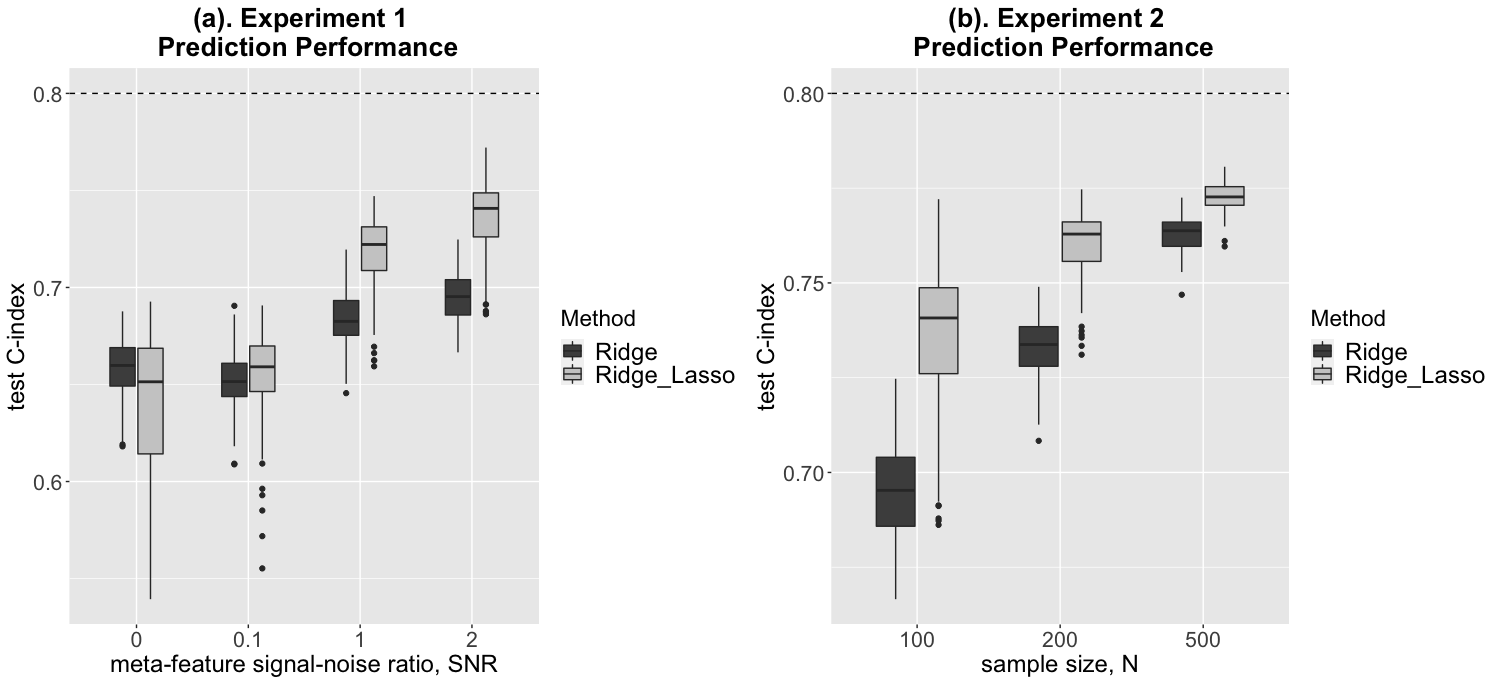
\includegraphics[width=\textwidth]{C12}
    \caption{Simulation: `xrnet' prediction performance (i)}
    \label{fig:C12}
\end{figure} 

\begin{figure}[H]
    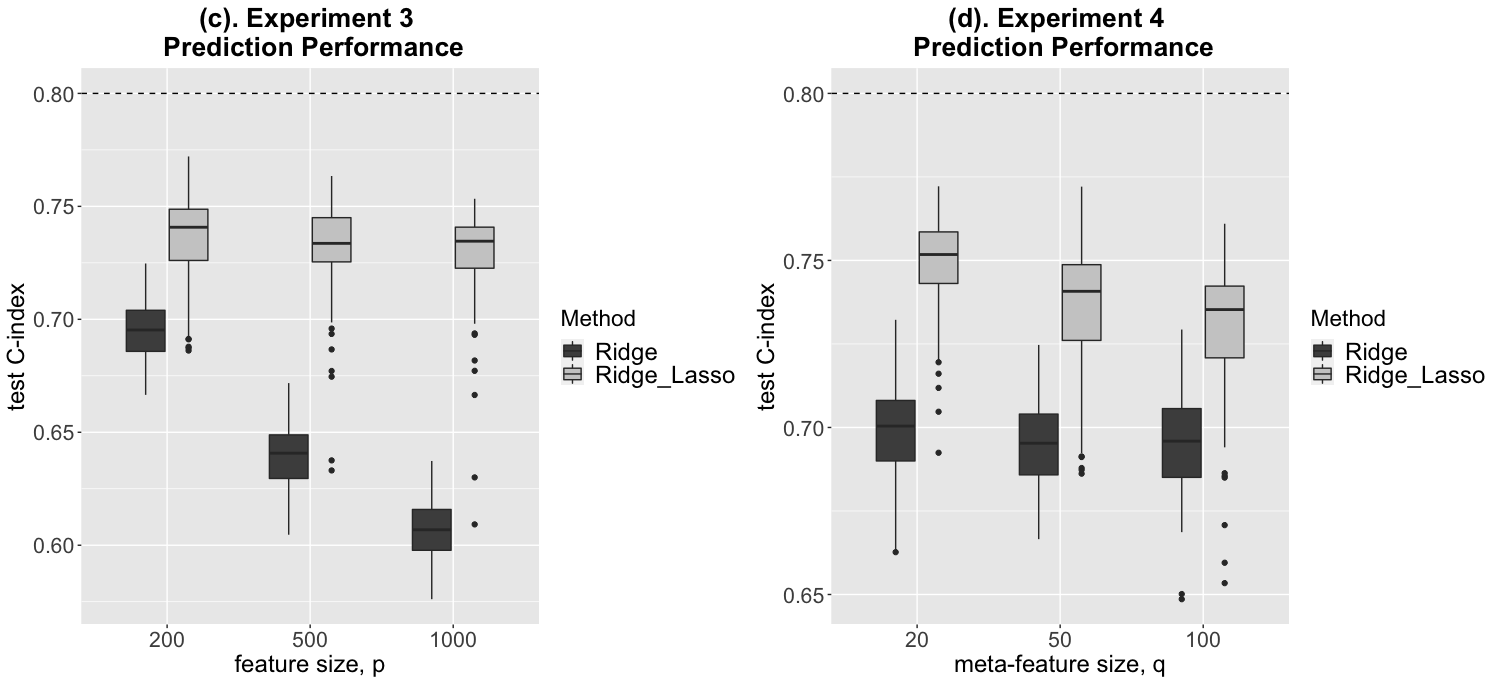
\includegraphics[width=\textwidth]{C34}
    \caption{Simulation: `xrnet' prediction performance (ii)}
    \label{fig:C34}
\end{figure} 

\begin{figure}[H]
    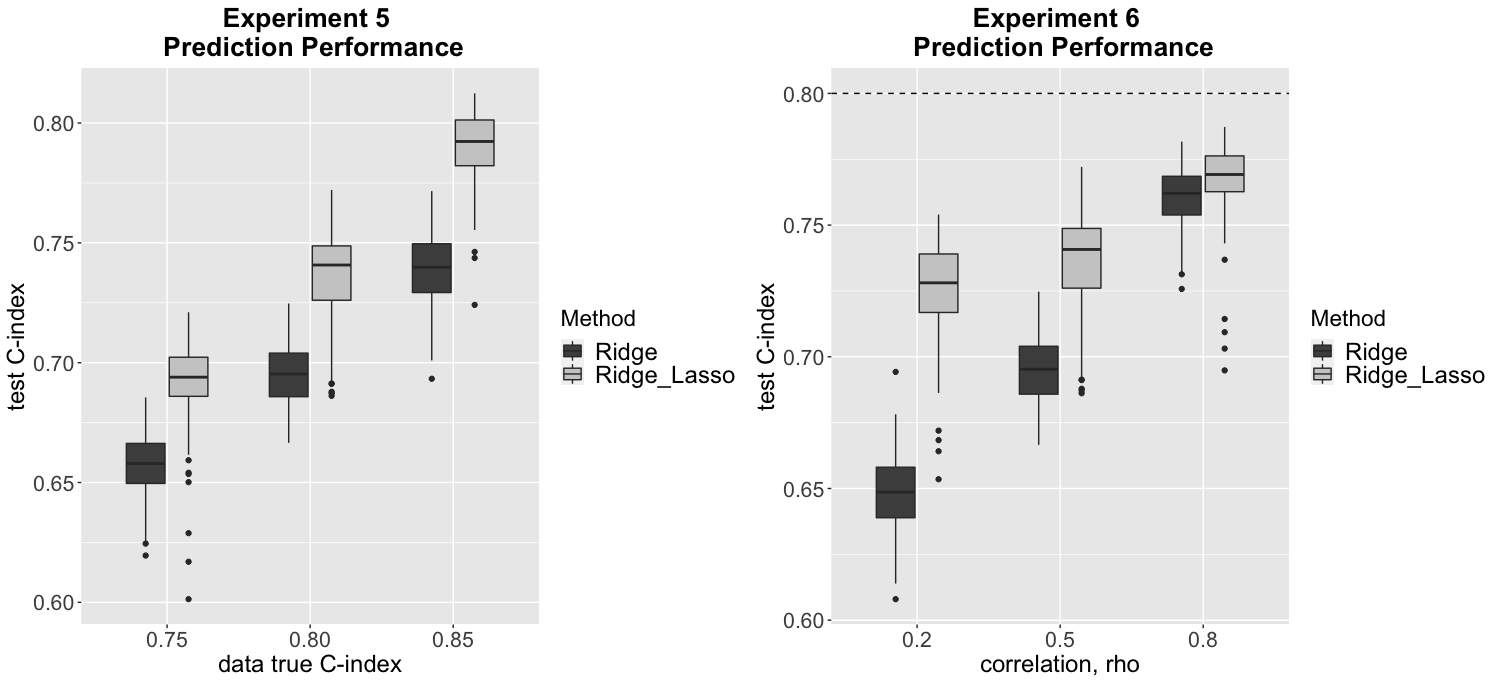
\includegraphics[width=\textwidth]{C56}
    \caption{Simulation: `xrnet' prediction performance (iii)}
    \label{fig:C56}
\end{figure} 

\begin{figure}[H]
    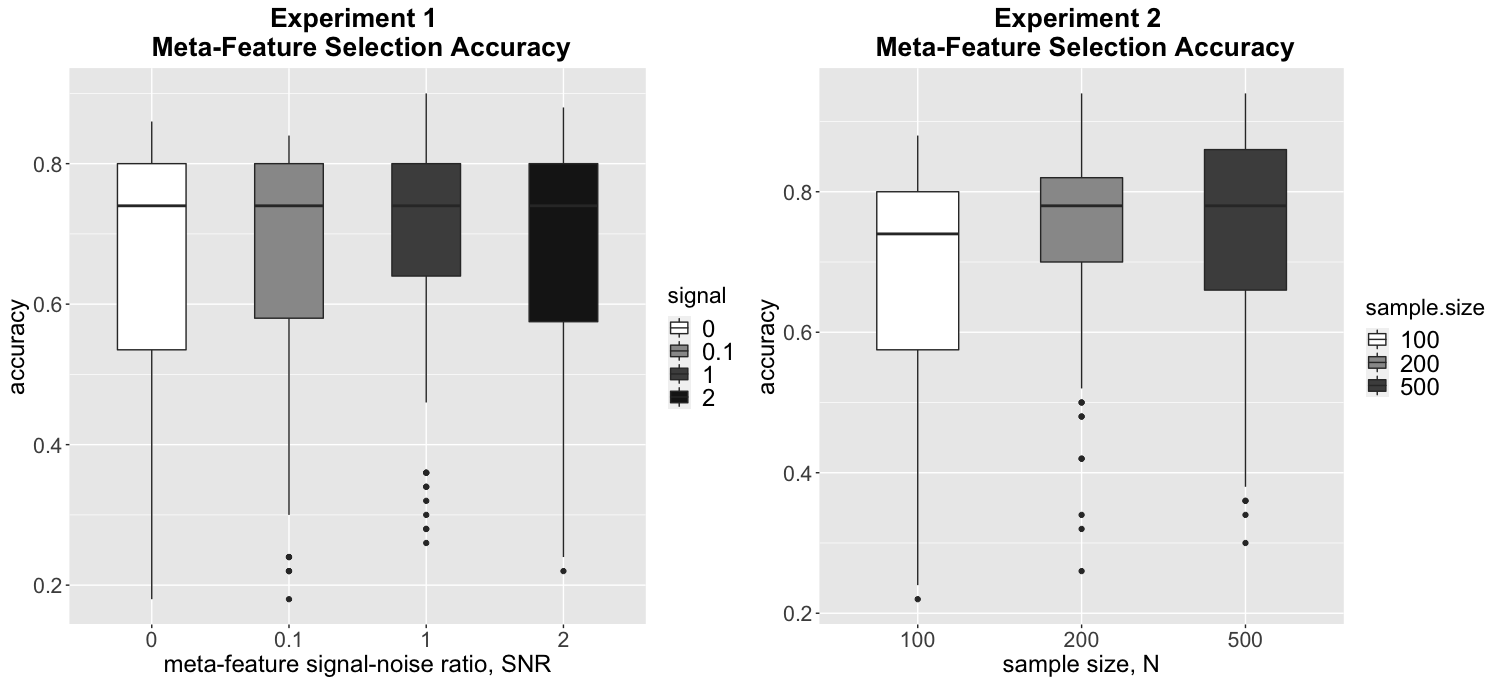
\includegraphics[width=\textwidth]{acc12}
    \caption{Simulation: `xrnet' meta-feature selection (i)}
    \label{fig:acc12}
\end{figure} 

\begin{figure}[H]
    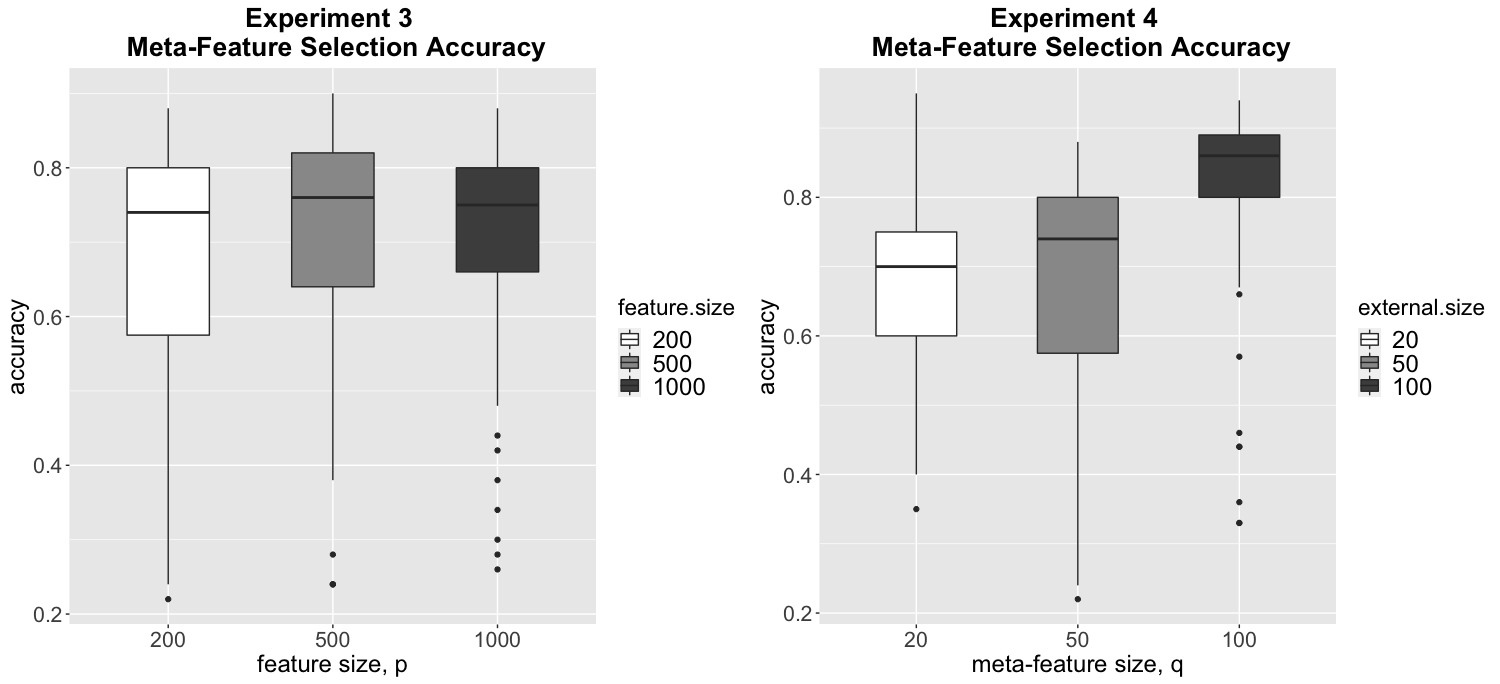
\includegraphics[width=\textwidth]{acc34}
    \caption{Simulation: `xrnet' meta-feature selection (ii)}
    \label{fig:acc34}
\end{figure} 

\begin{figure}[H]
    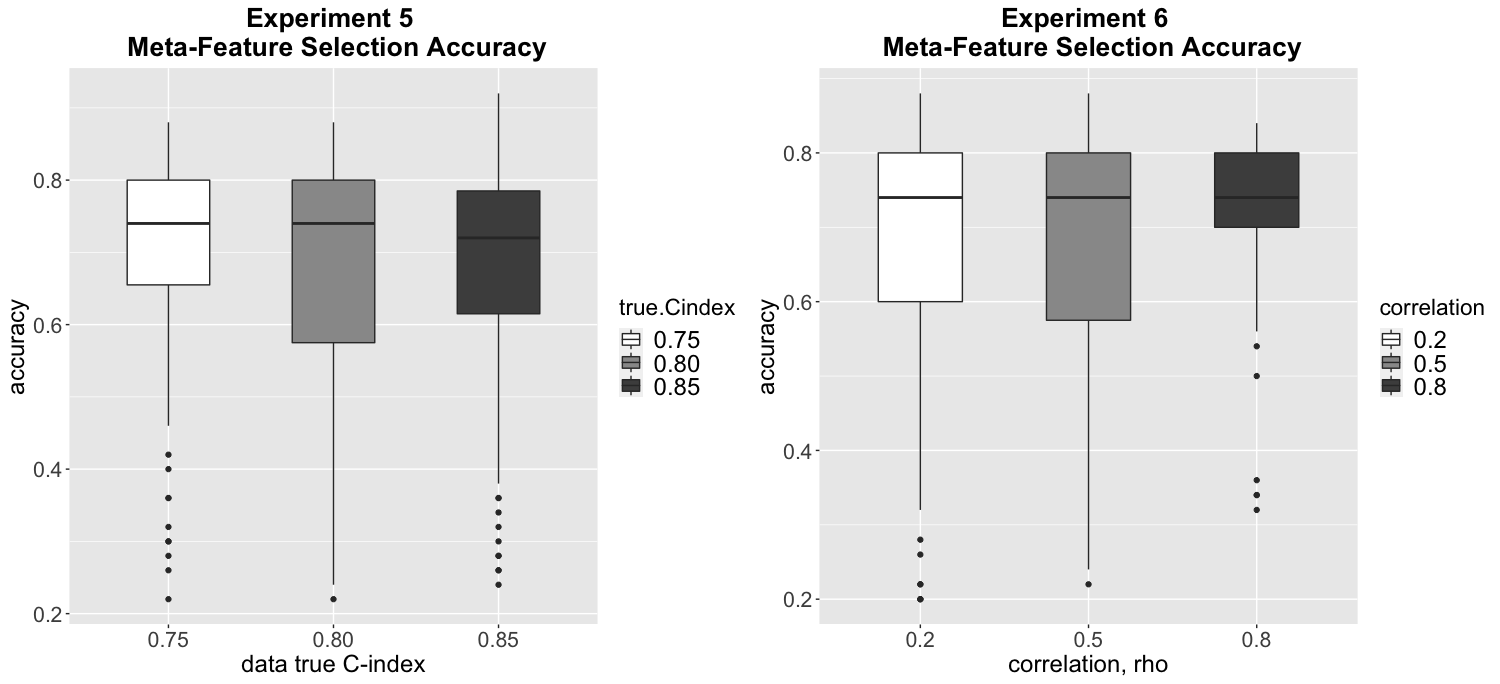
\includegraphics[width=\textwidth]{acc56}
    \caption{Simulation: `xrnet' meta-feature selection (iii)}
    \label{fig:acc56}
\end{figure} 

\section{Appendix for chapter 3}
\subsection{More simulation results}
We conducted 4 experiments for the meta-feature guided regularized regression model. The base case scenario is high meta-feature informativeness, sample size $N=100$, number of features $p=200$, number of meta-features $q=10$. In every experiment, we vary one of the 4 parameters and hold others fixed. We have seen the prediction performance results (Figure \ref{fig:sim21}), here we show feature selection accuracy, and number of features selected.

\begin{figure}[H]
    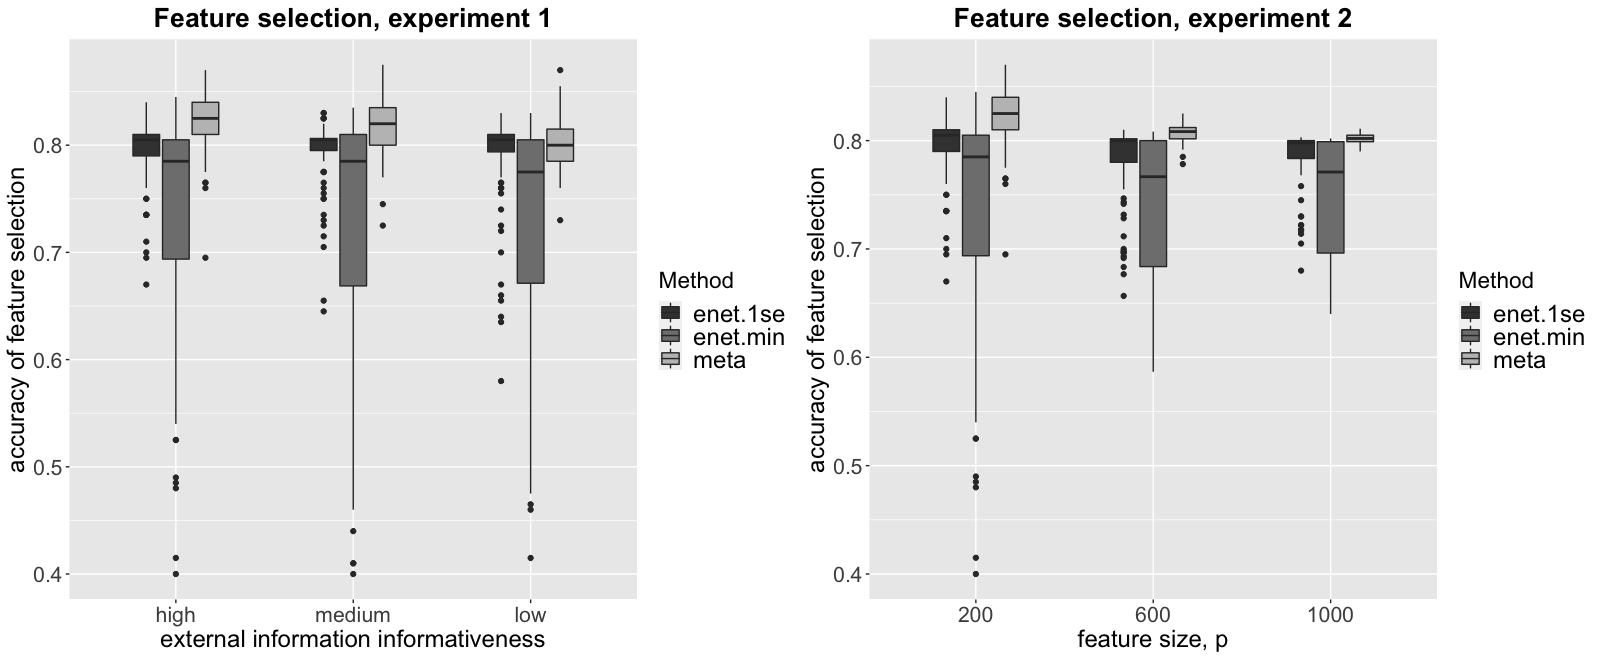
\includegraphics[width=\textwidth]{acc212}
    \caption{Simulation: meta guided feature selection accuracy (i)}
    \label{fig:acc212}
\end{figure} 

\begin{figure}[H]
    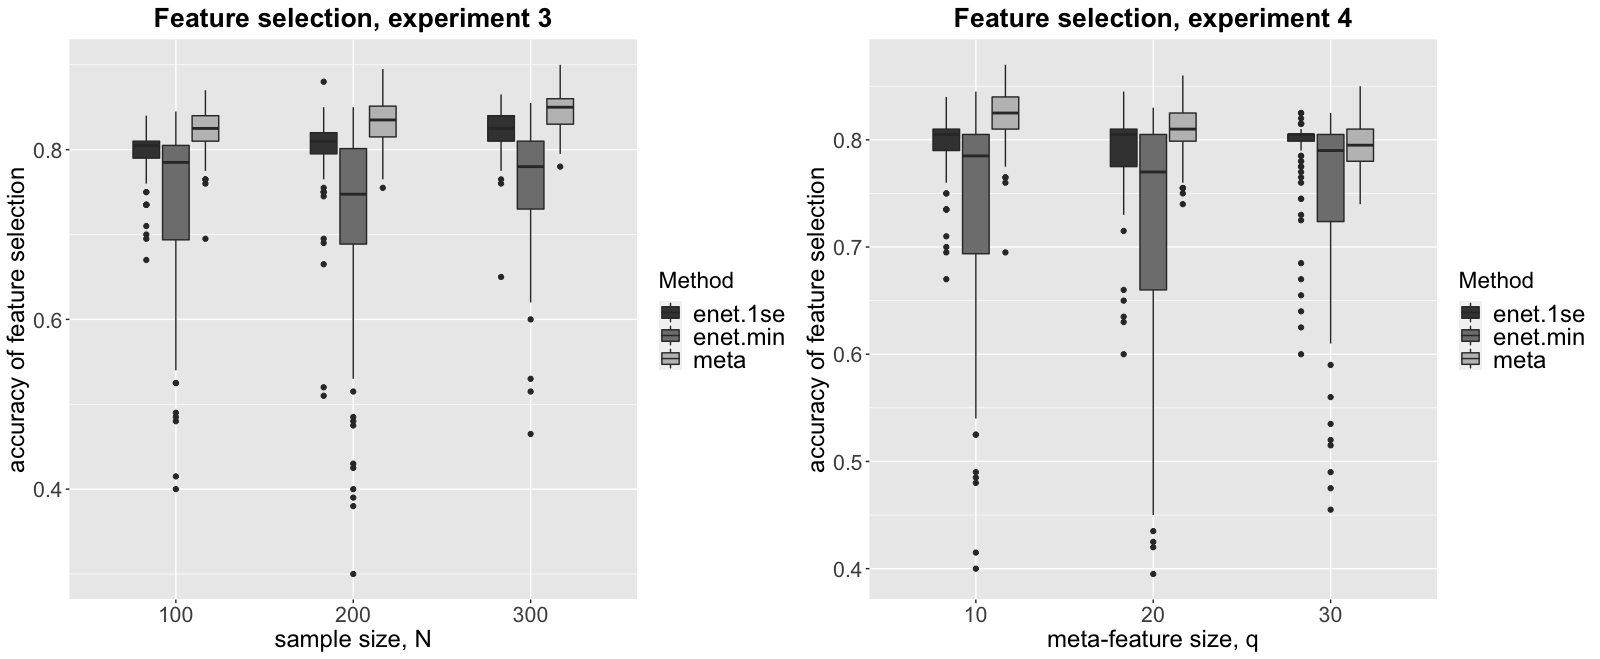
\includegraphics[width=\textwidth]{acc234}
    \caption{Simulation: meta guided feature selection accuracy (ii)}
    \label{fig:acc234}
\end{figure} 

\begin{figure}[H]
    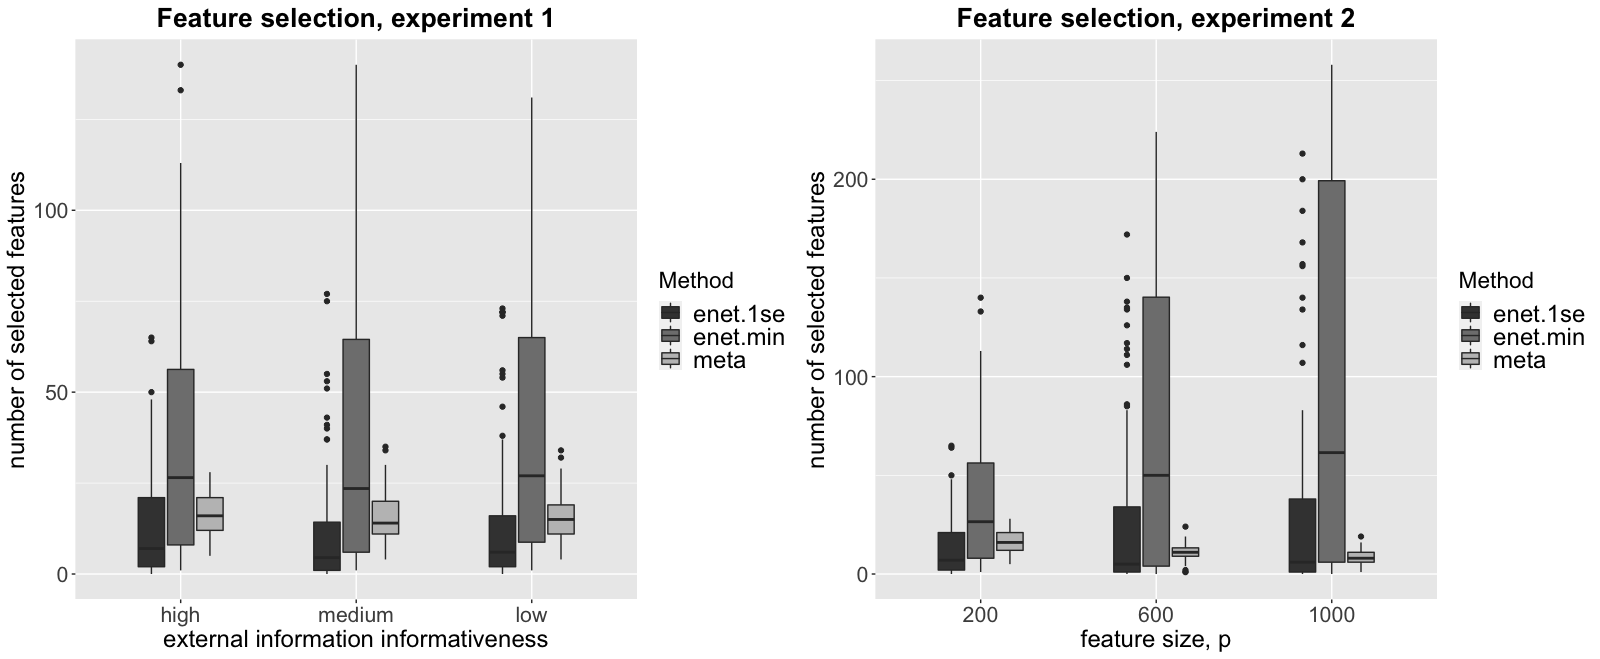
\includegraphics[width=\textwidth]{sel212}
    \caption{Simulation: meta guided number of selected features (i)}
    \label{fig:sel212}
\end{figure} 

\begin{figure}[H]
    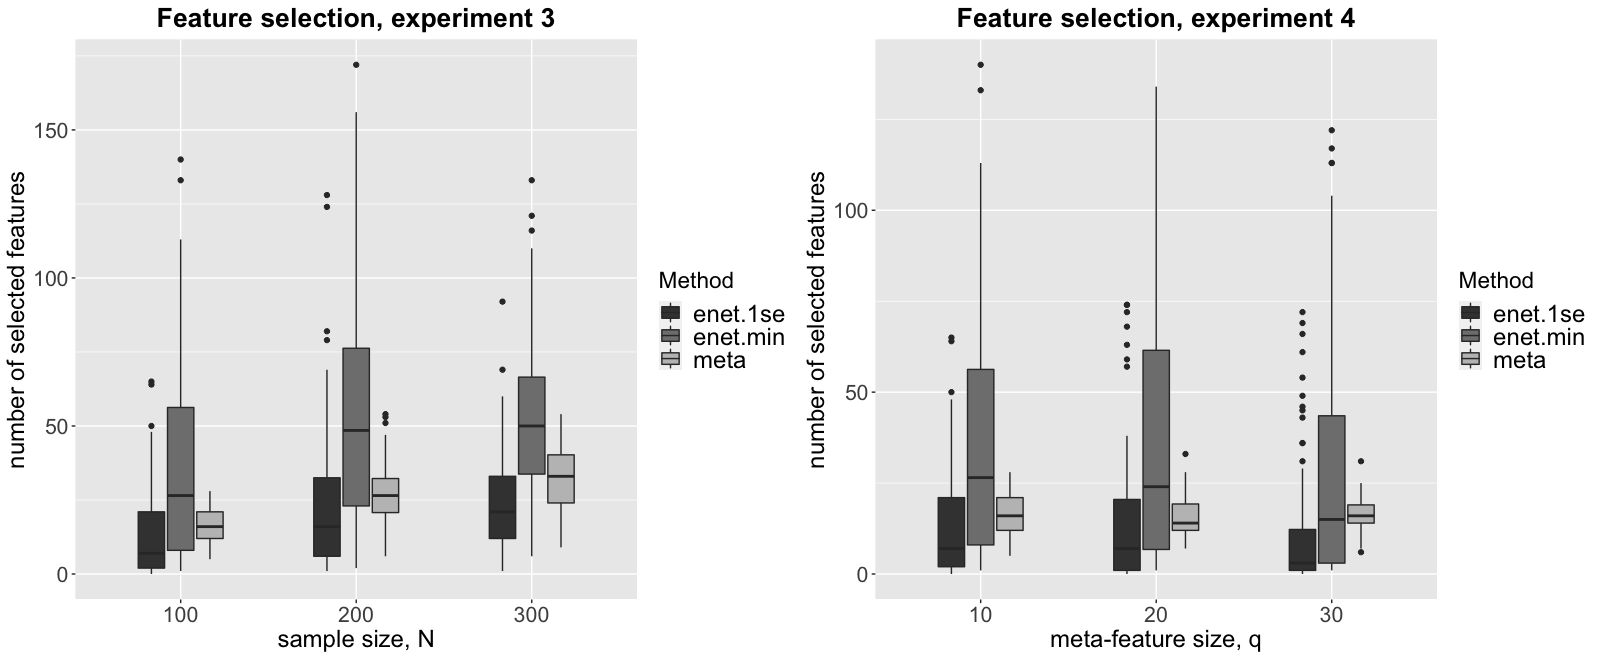
\includegraphics[width=\textwidth]{sel234}
    \caption{Simulation: meta guided number of selected features (ii)}
    \label{fig:sel234}
\end{figure} 


\endgroup

% In case your dissertation has multiple volumes.
% \addvolumecontents{thesis_part2}
% \addvolumecontents{thesis_part3}
% \addvolumecontents[lof]{thesis_part2}

\end{document}
